%%%%%%%%%%% Preamble
\documentclass[a4paper,12pt]{article}
\usepackage[longnamesfirst, round]{natbib}  
%\usepackage[latin1]{inputenc}   
\usepackage[utf8]{inputenc}

\usepackage[T1]{fontenc}        
\usepackage{color}              
\usepackage{amsmath,amsfonts,amssymb}
\usepackage{bm}
%\usepackage{ngerman}           
\usepackage[english]{babel}                     
\usepackage{graphicx}           
\usepackage{epstopdf}
\usepackage{longtable}          
\usepackage{booktabs}
\usepackage[flushleft]{threeparttable}
\usepackage{multirow}         
\usepackage{url}
\usepackage[hidelinks]{hyperref}
\usepackage{xcolor}
% \hypersetup{
%   colorlinks   = true, %Colours links instead of ugly boxes
%   urlcolor     = blue, %Colour for external hyperlinks
%   linkcolor    = blue, %Colour of internal links
%   citecolor   = black %Colour of citations
% }
\hypersetup{ hidelinks, }
\usepackage{caption}
\usepackage{subcaption}
\usepackage{wrapfig}
\usepackage{rotating}
\usepackage{graphicx,wrapfig}
\usepackage{tabularx}
\usepackage{multirow}
\usepackage[section]{placeins}
\usepackage{newtxmath,newtxtext}
\usepackage{setspace}
\usepackage[subtle]{savetrees}


%%%%%%%%%%%% Document Definitions
\usepackage[margin=2.5cm]{geometry}  %define margins
%\oddsidemargin 2.5cm \evensidemargin 0.1in \textwidth 15.5cm \topmargin -0.4in \textheight 24.5cm
\pagestyle{plain}    
\parindent 0cm     
\pagestyle{plain}        
\newcommand{\bs}{\boldsymbol}  %bold symbols
\DeclareMathOperator*{\argmin}{arg\,min} % redefine argmin for better appearance
%\renewcommand{\baselinestretch}{1.25}  1.5 spacing for standard Latex font
\setstretch{1,4} % 1,5 spacing for Times new Roman 
% -> see: https://tex.stackexchange.com/questions/442030/setting-spaces-with-titlespacing-and-fonts
\begin{document}
\setlength{\abovedisplayskip}{6pt}
\setlength{\belowdisplayskip}{6pt}

%%%%%%%% Title page of examination office
\clearpage

\begin{center}
\vspace*{2cm}

\Large\textbf{Disentangled Visual Attribute Manipulation in Fashion:
Techniques in Generative Deep Neural Networks}\\[0.5cm]
\rule{13cm}{0.4pt}\\[1.5cm]

\large\textbf{Degree Dissertation\\
for the\\
Master Examination in Data Science in Business and Economics\\
at the\\
Faculty of Economic and Social Sciences\\
of the\\
Eberhard Karls Universität\\
Tübingen}\\[2cm]
\end{center}

\begin{flushright}
Examiner:\\
Dr. Aseem Behl\\[1.5cm]

Submitted by:\\
Malte Genschow\\
Born in Filderstadt\\[1.5cm]

Date of submission: 28/08/2024\\
\end{flushright}

\thispagestyle{empty}
\setcounter{page}{0}

\newpage


%%%%%%%%%%% Title Page
\pagenumbering{roman}   
\begin{titlepage}       
\thispagestyle{empty}   
\begin{center}
\large Faculty of Economics and Social Sciences \\of the University of Tuebingen \\
\vspace*{1cm}
{Master Thesis} \\
\vspace*{2.5cm}
{\bf  \large Disentangled Visual Attribute Manipulation in Fashion: \\ Techniques in Generative Deep Neural Networks} \\
\vspace*{3cm} 

Dr. Aseem Behl \\
\vspace*{0.5cm} 
\normalsize {Summer Term 2024} \\
\vspace*{0.5cm} 
 %\today\\
\end{center}


%		Information about the author of the thesis
\vfill
\begin{footnotesize}
    

\begin{minipage}[t]{0.5\linewidth}
  Malte Genschow \\
  Hanna-Bernheim-Str. 46 \\
  72072 Tuebingen \\
  Phone: 015784765887 \\
  E-Mail: malte.genschow@student.uni-tuebingen.de
 \end{minipage}
\begin{minipage}[t]{0.5\linewidth}
  Study Program: \\
  Data Science in Business and Economics (M.Sc.) \\
  5th semester \\
  Matriculation Number: 3891245 \\
  Date of Submission: 
  August 28, 2024
 \end{minipage}

\end{footnotesize}
\end{titlepage}
\newpage      

%%%%%%%%%%%%%%%% Abstract
%\clearpage

\begin{center}
    \textbf{Abstract}
\end{center}
The rapid evolution of generative adversarial networks (GANs) has significantly impacted various domains, including fashion, where design typicality is a critical factor in consumer preference. This study explores the disentangled manipulation of visual attributes, specifically design typicality, using generative models within the fashion industry. A comprehensive pipeline was developed utilizing a custom-trained StyleGAN2-Ada model and multiple GAN inversion techniques to perform fine-grained manipulations on dress designs. Two methods for measuring typicality were introduced: a simple approach using DINOv2 embeddings and a more complex method employing disentangled embeddings with a focus on specific fashion attributes. The results demonstrate the effectiveness of the proposed typicality manipulation techniques, both with and without conditioning on physical attributes like color and sleeve length. The implications of these techniques extend to enhancing design processes by optimizing fashion items for increased consumer appeal, bridging the gap between aesthetic attribute manipulation and practical design augmentation in the fashion domain.

\newpage

%%%%%%%%%%%%% Table of Contents
\tableofcontents
\listoffigures
\listoftables
\newpage
\newcommand{\abbrlabel}[1]{\makebox[3cm][l]{\textbf{#1}\ \dotfill}}
\newenvironment{abbreviations}{\begin{list}{}{\renewcommand{\makelabel}{\abbrlabel}}}{\end{list}}
\section*{Abbreviations}
\begin{abbreviations}
\item[DCGAN] Deep Convolutional Generative Adversarial Network
\item[e4e] Encoder 4 Editing
\item[FID] Fr\'echet Inception Distance
\item[GAN] Generative Adversarial Network
\item[IS] Inception Score
\item[KID] Kernel Inception Distance
\item[LoRA] Low-Rank Adaptation
\item[LPIPS] Learned Perceptual Image Path Similarity
\item[MSE] Mean Squared Error
\item[PCA] Principal Component Analysis
\item[PGGAN] Progressive Generative Adversarial Network
\item[PTI] Pivotal Tuning Inversion
\item[SSIM] Structural Similarity Index Measure
\item[SVM] Support Vector Machine
\item[VAE] Variational Autoencoder
\end{abbreviations}
\newpage



%%%%%%%%%%%%%%%%% Main Body
\pagenumbering{arabic}      
\setcounter{page}{1}  

\section{Introduction}
The rapid development of generative neural networks for image generation has not only pushed the boundaries of computer vision research but also opened up new possibilities for productivity increases in many industries with drastic economic implications. McKinsey estimates, that only in product research and design, generative models could unlock \$60 Billion in productivity \citep{mc_kinsey_report}. Using generative models as assistants in the design process and thus automating parts of the value creation chain can hugely increase industrial productivity \cite[p.1]{regenwetter2022deep}. At the same time, many products are highly dependent on innovative or brand-specific designs, and especially in the fashion industry, the designer's experience and professional knowledge play an important role in the design process \cite[p.3]{sharma2021development}. However, generative models can augment these experts' design process and help them align their designs with the newest insights from consumer behavior research. In this work, one example of such a design augmentation for fashion designers is developed, focusing on the design typicality of fashion products. Research in consumer behavior has consistently demonstrated the significant role that typicality plays in product evaluation. Products are generally evaluated more positively, if they are more typical since typical products can be easier categorized by consumers (see \cite{barsalou1985ideals} p.1, \cite{sujan1985consumer} p.43) and processed more fluently (see e.g. \cite{veryzer1998influence} p.1, \cite{winkielman2006prototypes}, p.1). Additionally, more typical designs are more prevalent in consumers' everyday lives and can thus benefit from repeated exposure which can further increase consumer liking and familiarity \citep[p.23]{zajonc1968attitudinal}. In addition, consumers perceive atypical products as less reliable and functional than typical ones \cite[p.613]{schnurr2017impact}. Interestingly, the relationship between typicality and consumer liking is not linear. While more typical products can be categorized more easily which leads to higher consumer preferences, this only works to a certain extent. \cite{meyers1989schema} found that products which are moderately incongruent with the schema of their category (i.e. moderately atypical) are preferred over extremely incongruent products and completely congruent products. Products that are entirely congruent with the category schema are perceived as not noteworthy and exhibit lower consumer preference \cite[p.40]{meyers1989schema}. Furthermore, \cite{liu2017effects} found that moderate levels of typicality exhibit the highest consumer preferences with decreasing preferences for very high and very low typicality levels. \\
Keeping product typicality in mind is therefore central to the design process, as it directly influences consumer perceptions and decision-making processes. While expert human designers can focus on their individual design process, novel technologies from the domain of generative models can support optimizing a finished design regarding its design typicality for increased consumer preferences. Such a model could edit a design such that it is more (or less) typical than the initial draft by the designer, thus increasing consumer liking. Since the overall design of the fashion item should not change significantly, only minor and very targeted manipulations in the design are desired. This requires a very targeted and fine-grained image manipulation technique that can edit \textit{aesthetic} attributes, e.g. typicality, of the design in a disentangled manner (i.e. without altering other attributes). There are multiple works that research design augmentation for \textit{physical} attributes like sleeve length or color of fashion items (e.g. \cite{choi2023developing}, \cite{chen2020tailorgan}, \cite{ping2019fashion}, \cite{kwon2022tailor}). Furthermore, there is literature on \textit{aesthetic} attribute manipulation in other domains using generative neural networks. For example, \cite{goetschalckx2019ganalyze} manipulates images regarding visual attributes like memorability or emotional valence. To the best of the author's knowledge, a disentangled and targeted manipulation technique for aesthetic attributes like design typicality does not exist yet. Therefore, the goal of this work is the 
\begin{itemize}
    \item development of a fine-grained typicality manipulation method for aesthetic attributes and
    \item the exploration of generative models, GAN inversion methods, and latent space manipulation techniques to achieve this goal.
\end{itemize} 
The main contribution of this work is the development of a model that connects the research on aesthetic attribute manipulation using generative models and design augmentation in the fashion domain. While typicality is an \textit{aesthetic} attribute, manipulation of the design typicality may involve implicit manipulation of \textit{physical} attributes. The main difference to the works above, however, is the implicitness of \textit{physical} attribute manipulation, as the manipulation is targeted towards an \textit{aesthetic} attribute (typicality) which may result in manipulations of multiple \textit{physical} attributes of the fashion item.\\
To achieve the disentangled and targeted aesthetic attribute manipulation, a custom generative adversarial network (GAN), namely StyleGAN2-Ada \citep{stylegan2ada}, is trained for the garment category of women's dresses. Furthermore, multiple GAN-inversion models are tested and the best models are selected. To assess the typicality of a dress, two alternative typicality measurements are developed and in a final step, real dresses are manipulated using a latent space editing technique. The remainder of this work is organized as follows: Section 2 reviews the necessary preliminaries and relevant literature. Section 3 details the training data while section 4 explains the methodology, covering generation, inversion, typicality measurement, and latent space manipulation. Section 5 presents the results of each sub-method and the overall typicality manipulation. Section 6 discusses the method and results, and Section 7 concludes the paper.






 



\section{Background and Literature Review}
\subsection{Architecture Selection}
In the landscape of deep generative modeling, Variational Autoencoders (VAEs), Generative Adversarial Networks (GANs), and Diffusion models are the most commonly used architectures. While each of them has its strengths and weaknesses, I opt for the use of GANs. The main reasons for this will be described in this section. Since the goal of this thesis is to achieve highly controllable manipulations of visual attributes, having a well-defined, controllable, and interpolable latent space is a key requirement for the architecture. While both VAEs and GANs have such a latent space, VAEs lack the power to produce high-quality reconstructions \citep[p.2]{muller2024disentangling} and clear images \citep[p.1]{wang2020state}. Diffusion models on the other hand can produce high-fidelity images but have a highly unstructured latent space that lacks semantic meaning. Naively interpolating the latent space, as it is possible for GANs, leads to random and abrupt flickering and drastic changes in the generated image from diffusion models \citep[p.2]{zhang2024diffmorpher}. Making the latent space of diffusion models interpolable requires extensive efforts as e.g. \cite{zhang2024diffmorpher} has shown by interpolating between the LoRA \citep{hu2021lora} adaptions of two images. Another approach would be to interpolate between encodings of text prompts obtained using textual inversion in text-guided diffusion models like \cite{wang2023interpolating} have done. In general, a controllable and interpolable latent space with effortless learning of semantic meaning is possible only using GAN architectures. Furthermore, although GANs generally achieve less mode coverage (i.e. diversity) in their generations than VAEs and diffusion models \citep[p.1]{xiao2021tackling}, this does not pose a problem, since the application in this work builds on the narrow distribution of packshot images of dresses.
\subsection{GANs}\label{sec:gans}
Generative adversarial networks (GANs), first proposed by \cite{goodfellow2014generative}, have revolutionized the field of generative modeling in deep learning. A GAN consists of two adversarial models, a \textit{Generator} $G$ and a \textit{Discriminator} $D$. The generator aims to capture the data distribution and thus be able to produce data that mimics the real data. It takes data sampled from a prior distribution $\mathcal{Z}$, often a Gaussian distribution, and learns a function to map it into the data space. The discriminator model $D$ simultaneously aims to distinguish between data from the real distribution and data generated by $G$. To enable $G$ to learn the real data distribution and $D$ to improve its discriminative power, a non-cooperative two-player minimax game is used in combination with simultaneous gradient descent \citep[p.5]{saxena2021generative}. The objective function of a basic GAN model uses two objectives: Parameters of $D$ ($\theta_D$) are chosen such that the negative log-likelihood for binary classification is minimized and parameters of $G$ ($\theta_G$) are chosen such that the generated examples have a high probability of being real \citep[p.6]{saxena2021generative}. Thus, the overall objective function can be formulated as
\begin{equation}
\label{eq:basic_gan_loss}
\min_{\theta_G} \max_{\theta_D} V(G, D) = \min_G \max_D \mathbb{E}_{x \sim p_{\text{data}}} [\log D(x)] + \mathbb{E}_{z \sim p_z} [\log (1 - D(G(z)))]
\end{equation}
 where $V(G,D)$ is a binary cross entropy function \citep[p.6]{saxena2021generative}. In the beginning, none of the networks has any knowledge about the domain \citep[p.2]{bermano2022state}. The models improve by learning from each other. \cite{bermano2022state} describe the training as a repetitive process, in which the generator tries to fool the discriminator which in turn learns to recognize this strategy. This training scheme allows the model to learn via self-supervision and interestingly, the generator learns to generate high-fidelity images without ever seeing a single real image \citep[p.2]{bermano2022state}. As an extension, \cite{mirza2014conditional} introduced a conditional GAN architecture, where a conditioning of a single class of the domain can be achieved in both the generator and discriminator. Since in this work I focus on across-class manipulations, unconditional architectures are used which can capture the multimodal distribution of multiple classes in one model. The basic GAN architecture can be seen in figure \ref{fig:gan_architecture}.
 
\begin{figure}[ht]
    \centering
    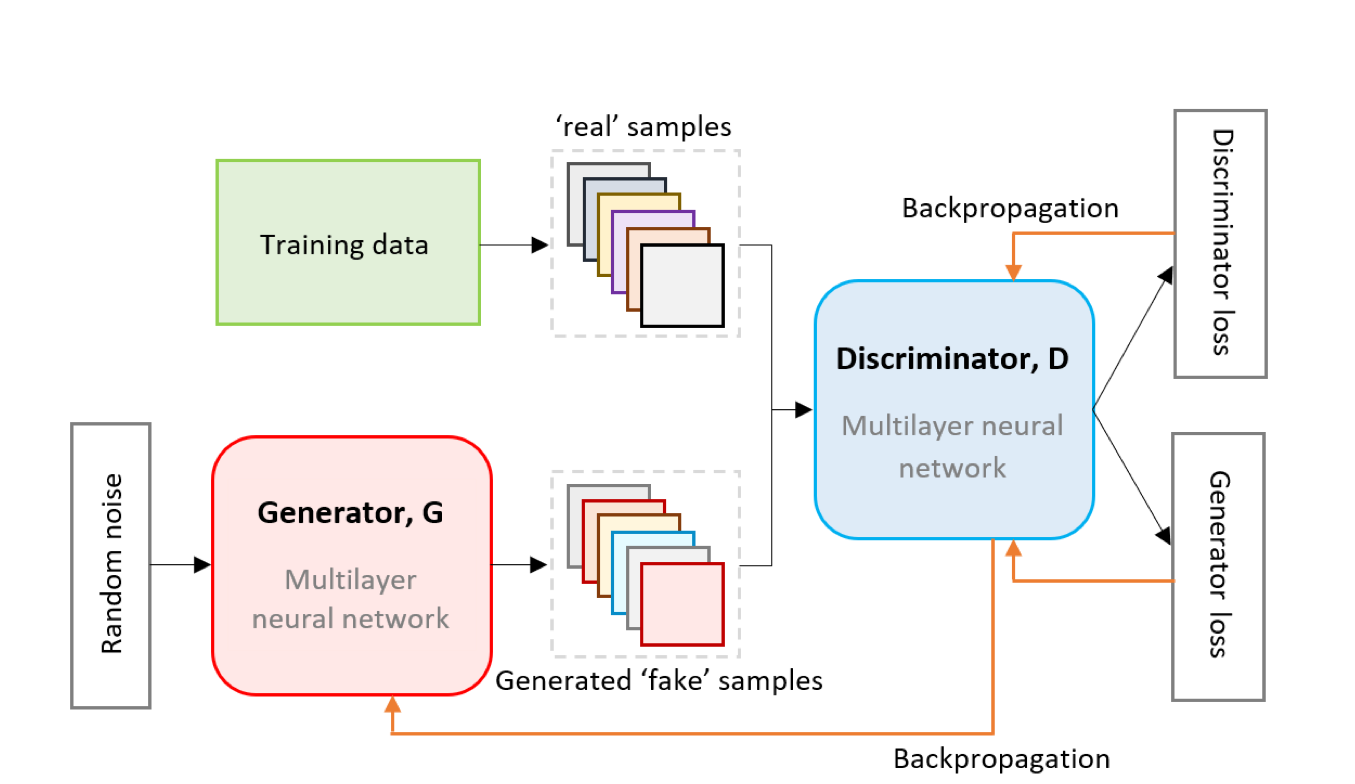
\includegraphics[width=0.8\linewidth]{Thesis/Background/assets/basic_gan_architecture.png}
    \caption[Basic GAN architecture]{Basic GAN architecture - taken from \cite{little2021generative}} 
    \label{fig:gan_architecture}
\end{figure}
% While all GAN architectures share the concept of two adversarial networks, there are many combinations of generator architectures, discriminator architectures, loss functions, and optimization algorithms. Most image generation architectures use deep neural networks for both the generator and discriminator. Given the vastness of GAN architectures, I will focus on the key improvements relevant to the architecture used in this work. DCGAN, proposed by \cite{radford2015unsupervised}, uses deep convolutional networks in the generator and discriminator, forming the foundation for many subsequent high-fidelity image generation GANs. \cite{arjovsky2017wasserstein} and \cite{gulrajani2017improved} introduced improvements in discriminator loss formulation and optimization. Since the standard GAN loss can lead to vanishing gradients with a strong discriminator \citep[p.2]{gulrajani2017improved}, they proposed using the Earth-Mover (Wasserstein) distance, resulting in the Wasserstein-GAN (WGAN), which is also used in StyleGAN. Another frequently used GAN family is based on ProGAN or progressive GAN (PGGAN), which employs a progressive growing strategy to incrementally improve the resolution of both the generator and discriminator, learning increasingly finer features \citep{karras2017progressive}. Many design choices from PGGAN, such as progressive growing, laid the foundation for StyleGAN's success.
While all GAN architectures share the concept of two adversarial networks, there are many combinations of generator architectures, discriminator architectures, loss functions, and optimization algorithms. Numerous architectures have gradually improved the image quality and training stability of GANs (e.g. DCGAN \citep{radford2015unsupervised}, WGAN \citep{arjovsky2017wasserstein}, PGGAN \citep{karras2017progressive}). The final breakthrough of image generation using GANs, however, happened with the introduction of StyleGAN \citep{stylegan1}. \\
The \textbf{StyleGAN family} (e.g., \cite{stylegan1}, \cite{stylegan2}, \cite{stylegan2ada}) has achieved an unprecedented level of image quality and fidelity \citep[p.1]{tov2021designing}. StyleGAN has become the state-of-the-art GAN architecture, and the golden standard for facial image editing \cite[p.1]{bermano2022state}. Its dominance is due to design choices that create a well-organized, smooth, and highly disentangled latent space that exhibits a semantic understanding of the target domain merely through the effect of inductive bias \citep[p.6]{bermano2022state}. A key innovation in StyleGAN is the mapping network $f: \mathcal{Z} \rightarrow \mathcal{W}$, which transforms Gaussian-distributed latent codes from $\mathcal{Z}$ into an intermediate latent space $\mathcal{W}$, ensuring better alignment with the real data distribution. This mapping allows the model to account for the non-uniform distribution of image attributes by "unwrapping" the latent space, making it more linear and easier to manage \citep[p.6]{stylegan1}. As a result, the generator can more effectively disentangle and recreate various image features, enhancing the quality and diversity of the generated images. The main component in StyleGAN's architecture is the style modulation layers that allow precise control of the "style" in generated images. The latent codes in $w$ are transformed to "styles" $\bm{y} = (y_s, y_b)$ using learned affine transformations. Using these transformations, different dimensions of the StyleGAN latent space $\mathcal{W}$ are injected at different levels of the synthesis process, allowing targeted variation at the coarse, medium, and fine details of the generated image \citep[p.4]{stylegan1}. 
\begin{wrapfigure}{r}{7cm}
    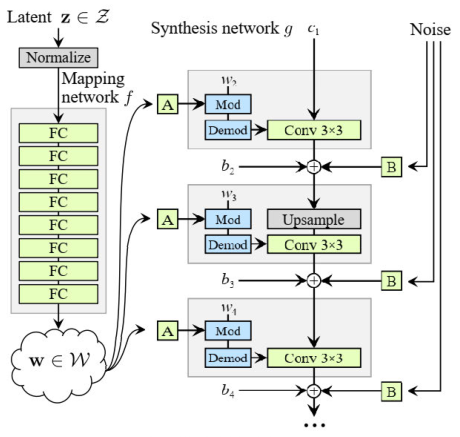
\includegraphics[width=1\linewidth]{Thesis/Background/assets/sg2_schema-cropped.pdf}
    \caption[StyleGAN2 Architecture]{StyleGAN2 Architecture - taken from \cite{hermosilla2021thermal}}
    \label{fig:stylegan2_schema}
\end{wrapfigure} 
Additionally, by injecting random noise into each layer of the synthesis network, stochastic variation in the output is ensured \citep[p.1]{stylegan2}. \\
\textbf{StyleGAN2}, an improved version of the original StyleGAN, introduces enhancements that address artifacts and improve image quality by refining both the architecture and training processes \citep[p.2]{stylegan2}. 
A key change is the replacement of progressive growing with skip-connections in the generator and a residual discriminator \citep[p.6]{stylegan2}. 
This simplifies training by maintaining a fixed resolution throughout, eliminating the need for manual tuning as resolution increases. Another major improvement is the redesign of the style modulation layers through a modulation-demodulation operation. Here, style modulation is directly applied to the convolutional layer weights, followed by demodulation to normalize feature maps. 
This enhances the consistency and quality of the generated images. A detailed schema of the StyleGAN2 architecture is shown in figure \ref{fig:stylegan2_schema}. StyleGAN2 also introduces lazy regularization, computing regularization losses every 16 minibatches, which reduces computational cost and training time \citep[p.5]{stylegan2}. 
Additionally, the novel path length regularization ensures that small changes in the latent code $w \in \mathcal{W}$ lead to smooth, small changes in the generated image. This regularizer penalizes large variations in the perceptual space of consecutive latent codes during training, resulting in more reliable models and smoother generators, which are easier to invert \citep[p.5]{stylegan2}. Since the model in this work needs to produce subtle changes when manipulating images, smooth latent space interpolation, achieved by StyleGAN2's path length regularizer, is crucial.

\textbf{StyleGAN2Ada} \citep{stylegan2ada} is a modified version of StyleGAN2 which introduces adaptive data augmentation techniques to address overfitting and improve generalization. Training GANs with a small dataset can easily lead to discriminator overfitting and thus training of the generator fails due to vanishing gradients. Using adaptive discriminator augmentations, the authors can stabilize training on small datasets and show that only a few thousand images are needed to train StyleGAN2Ada \citep[p.1]{stylegan2ada}. This is achieved through the use of an adaptive augmentation pipeline that introduces random transformations, such as translation, rotation, and color jittering, only when the discriminator begins to overfit. Since in this work, a limiting factor is the access to high-quality training data, using StyleGAN2Ada is the logical choice, as it allows training of a high-quality generator on a small sample. 







\subsection{GAN Inversion}\label{sec:gan_inversion}
While synthesizing arbitrary fake images from a pre-trained generator is straightforward, editing real images is a non-trivial task. For latent space editing techniques to be applied to real images, one must first find the corresponding latent code of the real image using a \textit{GAN Inversion} technique. Initially introduced by \cite{zhu2016generative}, the goal of GAN inversion is to find a latent code $w \in \mathcal{W}$ which most closely reconstructs the real image. Following \cite{bermano2022state}, inversion can be formally defined as: Given a pre-trained generator $G: \mathcal{W} \rightarrow \mathcal{X}$ and real image $x \in \mathcal{X}$,  GAN inversion aims to find $w \in \mathcal{W}$ such that 
\begin{equation}
\label{eq:gan_inversion}
    w^* =  \argmin_{w} \mathcal{L}(x, G(w)),
\end{equation}
where $\mathcal{L}$ is any reconstruction loss. Due to the non-convexity of the generator, this leads to a non-convex optimization problem. Approaches to solve this problem can be grouped into learning-/encoder-based, optimization-based, and hybrid methods \citep[p.6]{xia2022gan} and will be explained below. Note that inversion can be executed in any latent space ($\mathcal{Z}$, $\mathcal{W}$, etc.) of any GAN architecture. In the following, however, I will focus on the latent spaces of StyleGAN-based architectures. 

\subsubsection{Latent Spaces}
Choosing the latent space for the inversion is an important design choice since this space should allow a precise reconstruction while facilitating disentangled editing and other downstream tasks \citep[p.5]{xia2022gan}. For StyleGAN-based architectures, most inversion techniques use $\mathcal{Z}$, $\mathcal{W}$, $\mathcal{W^+}$, $\mathcal{S}$, $\mathcal{P_N}$ or $\mathcal{P_N^+}$. \\
The first latent space in StyleGAN is $\mathcal{Z}$-space which follows a normal distribution and thus has a closed-form definition. As the generator learns a mapping $\mathcal{Z} \rightarrow \mathcal{X}$, images from the GAN's latent space can easily be sampled from $\mathcal{Z}$ \citep[p.5]{bermano2022state}. By using the nonlinear mapping network $f: \mathcal{Z} \rightarrow \mathcal{W}$ of the StyleGAN architecture (see section \ref{sec:gans}), a distribution of $\mathcal{W}$ is learned, which better captures the distribution of the real data \citep[p.6]{stylegan1} and has better disentanglement than $\mathcal{Z}$ \citep[p.7]{shen2020interpreting}. \cite{abdal2019image2stylegan} propose an extension of $\mathcal{W}$, $\mathcal{W^+}$ to solve the limited expressiveness of $\mathcal{W}$ when representing real images in the inversion task. While in $\mathcal{W}$ space all rows of the 16x512-dimensional latent vector (for 512x512 output images) are identical, $\mathcal{W^+}$ allows for 16 different 512-dimensional style vectors that are inserted at different layers of the synthesis network. While allowing for more precise reconstructions due to higher expressiveness, using $\mathcal{W^+}$ can come at the expense of image quality, as operating in $\mathcal{W^+}$ makes regions in the latent space available, which are outside of the distribution the generator was trained on \citep[p.5]{bermano2022state}. As almost all latent space manipulation methods work with the more common $\mathcal{Z^{(+)}}$- and $\mathcal{W^{(+)}}$-spaces, inversion methods that use $\mathcal{S}$-space (\cite{wu2021stylespace}) or $\mathcal{P_N}$- and $\mathcal{P_N^+}$-space (\cite{zhu2020improved}) are not very relevant to this work. For a schematic overview of the StyleGAN latent spaces, see figure \ref{fig:latent_spaces} in the appendix. Note that in this work, inversion and manipulation in $\mathcal{Z}$, $\mathcal{W}$ and $\mathcal{W^+}$ have been performed and eventually it was decided to focus only on $\mathcal{W^+}$ due to its superior performance in the inversion process.


\subsubsection{Inversion Methods}
\textbf{Optimization-based} GAN inversion techniques (e.g. \cite{yeh2017semantic}, \cite{creswell2018inverting}, \cite{gu2020image}, \cite{bau2020semantic}, \cite{lipton2017precise}) derive the latent vector for a given image by solving equation \ref{eq:gan_inversion} on an instance level. While this achieves high reconstruction quality of the real input images, this comes at the cost of computational efficiency \citep[p.2]{alaluf2021restyle} and lower editability \citep[p.3]{tov2021designing}. Therefore, no optimization-based methods were implemented in this work.

%\subsubsection{Encoder-Based Methods}
\textbf{Encoder-based} GAN inversion approaches mostly train an encoder network $E(x, \theta_E)$ to obtain a mapping from the input image to its latent code. The objective function closely resembles this of an autoencoder pipeline where the decoder is the fixed generator for which the inversion network is obtained \citep[p.6]{xia2022gan}. The training objective can be defined following \cite{bermano2022state}, p.9 as: 
\begin{equation}
    \theta^*_E = \arg \min_{\theta_E} \sum_i \mathcal{L}(\bs x_i, G(E_{\theta_E}(\bs x_i))).
\end{equation}
There have been extensive efforts to encoder-based architectures since \cite{luo2017learning} first proposed an autoencoder-inspired approach (e.g. \cite{kim2021exploiting}, \cite{wang2022high}, \cite{shanyan2020collaborative}, \cite{pidhorskyi2020adversarial}, \cite{kang2021gan}, \cite{richardson2021encoding}, \cite{he2016deep}). The encoder model used in this work is the state-of-the-art encoder model encoder4editing (e4e), introduced by \cite{tov2021designing}. e4e was designed with a particular focus on editing capabilities of the inversion.
 By analyzing the trade-offs between distortion, perceptual quality, and editability, the authors can design an encoder that ensures editability while maintaining a high reconstruction quality. They find that editability and perceptual quality are high when an image is inverted close to $\mathcal{W}$ but lives in $\mathcal{W^+}$ to simultaneously achieve low distortion in the generation \citep[p.2]{tov2021designing}. This is achieved by adding multiple loss terms to the encoder. First, distortion is minimized by adding a similarity loss based on a ResNet-50 \citep{he2016deep} network, an $\mathcal{L}_2$ loss term, and a loss term based on LPIPS \citep{zhang2018unreasonable}. To maximize perceptual quality, a loss term is used to minimize the variation within the learned latent codes \citep[p.5]{tov2021designing}. Furthermore, a latent discriminator \citep{nitzan2020face} is employed to ensure proximity of the latent code to $\mathcal{W}$ \citep[p.5]{tov2021designing}. Encoder4editing poses an important basis for many inversion techniques. See figure \ref{fig:e4e} in the appendix for a schematic overview of the method. While encoder-based methods are considerably faster than optimization-based methods, their reconstructions are less accurate \citep[p.10]{bermano2022state}. To combine the fast inference time of encoders and the generally better performance of optimization models, several hybrid models have been proposed.


%\subsubsection{Hybrid Models}
\textbf{Hybrid models} obtain an initial latent code using an encoder and then further optimize this on a per-image level (e.g. \cite{zhu2016generative}, \cite{zhu2020domain}). Out of the universe of hybrid models, the most promising models based on the overall literature have been selected and tested in this work. These methods are explained below in more detail. \cite{alaluf2021restyle} propose \textbf{ReStyle}, an iterative approach, in which latent codes obtained from an e4e encoder are iteratively improved by learning residuals. Instead of obtaining the inversion from a single forward pass, the encoder is iteratively refined using a small number of steps that leverage a feedback algorithm between the predicted and the real image \citep[p.2]{alaluf2021restyle}. Each iteration computes a residual vector correcting the previous latent code, enhancing high-frequency details and complex structures.  This feedback mechanism allows intermediate reconstructions to better align with the target image, yielding lower LPIPS and MSE scores, while preserving semantic consistency and producing visually coherent results \citep[p.6]{alaluf2021restyle}. For a detailed schema of ReStyle see figure \ref{fig:restyle} in the appendix.

\cite{alaluf2022hyperstyle} propose \textbf{HyperStyle} which uses a hypernetwork-based encoder that learns offsets for the convolutional filters of the generator alongside the initial latent codes that are obtained from a fixed encoder (e.g. ReStyle). Thus, inference time is by a magnitude lower than for instance-level optimization while promising comparable reconstruction results \citep[p.5]{alaluf2022hyperstyle}. HyperStyle claims to bridge the gap between high-quality reconstructions that are obtained from generator-optimization approaches and fast inference time in encoder-based methods. Furthermore, the iterative refinement scheme introduced in ReStyle \citep{alaluf2021restyle} is adapted to the hyper-network training to achieve stronger expressive power and more accurate inversions \citep[p.5]{alaluf2022hyperstyle}. For a detailed schema of HyperStyle see figure \ref{fig:hyperstyle} in the appendix.

\cite{roich2022pivotal} propose \textbf{PTI}, a novel approach that combines initial inversions from an encoder and subsequent pivotal tuning of the generator, which achieved state-of-the-art performance in both distortion and editability. The initial latent code is obtained from an e4e model and thus lies within the well-behaved region of the latent space which allows editability \citep[p.2]{tov2021designing}. This code is used as a pivot around which the generator is trained for a few steps to better reconstruct the image while keeping nearby identities intact through a regularization term \citep[p.1]{roich2022pivotal}. While this achieves very high reconstruction quality and editability, it is also computationally expensive and complicates downstream tasks because each inversion needs its fine-tuned generator weights. 


\subsection{Manipulation}
While good inversion performance allows to accurately reconstruct a given image, the main goal of this work is to be able to consistently manipulate image attributes. Latent space manipulation is a research field closely connected to GAN inversion that aims at finding techniques to manipulate latent space representations of images such that the generated image from the manipulated latent space exhibits the desired edited attributes. Since the StyleGAN latent space is smoothly interpolable, moving in a carefully chosen direction in this space should also result in smooth interpolations in the desired semantic attributes \citep[p.6]{bermano2022state}. In general, semantic image manipulation using GANs can be performed using either specifically designed architectures based on conditional GANs or latent space manipulation techniques applied to pre-trained unconditional GANs. While models like StarGAN \citep{choi2018stargan} and StarGANv2 \citep{choi2020stargan} yield a more compact pipeline that does not require a specific model for each step, attributes have to be specified before training the generator. I chose to rely on an unconditional GAN model and additional latent space editing techniques since this approach is more general and yields better image quality \citep[p.2]{abdal2021styleflow}. Within those latent space navigation techniques, one can further differentiate between supervised (e.g. \cite{goetschalckx2019ganalyze}, \cite{shen2020interpreting}, \cite{wu2021stylespace}, \cite{yang2021discovering}) and unsupervised (e.g. \cite{ren2021learning}, \cite{yuksel2021latentclr}, \cite{harkonen2020ganspace}, \cite{shen2021closed}) approaches and between linear and non-linear (e.g. \cite{abdal2021styleflow}, \cite{li2023dystyle}, \cite{chen2022exploring}) approaches. The most important techniques will be briefly discussed below. \cite{harkonen2020ganspace} use an unsupervised approach by applying PCA on the latent space of a specific dataset. The principal components then correspond to specific attributes, however this annotation has to be done by manual inspection of resulting image manipulations. \cite{shen2021closed} proposed another unsupervised approach in which they use a semantic factorization method which is based on the principal components from the weights of the first layer of a pre-trained GAN. While unsupervised approaches may yield good results in the absence of labeled data, supervised approaches can leverage the information contained in the labels to find more accurate directions in the latent space. In one of the earlier works, \cite{goetschalckx2019ganalyze} propose a method to manipulate cognitive image properties like memorability. They achieve this by learning a transformer function that adds a learned direction to the initial latent code in $\mathcal{Z}$-space such that the assessor model at the end of the pipeline detects the altered memorability of the generated image. While this is a rather simple approach, it can be adapted to more complex workflows and other latent spaces. Building on the idea of learning a latent space offset based on assessor scores, \cite{shen2020interpreting} propose a technique that learns directions in latent space based on hyperplanes separating instances based on binary attributes. This method called InterFaceGAN will be explained in more detail in section \ref{sec:interfacegan}. While the above-mentioned methods mostly learn directions in latent space such that by traversing the latent space in this direction, the desired attribute changes in the output, non-linear approaches also yield promising results. StyleFlow, one of the most promising techniques, was proposed by \cite{abdal2021styleflow} and relies on normalizing flows that learn a mapping between $\mathcal{Z}$ and $\mathcal{W}$ conditioned on specific attributes. Manipulation is performed by reversing the mapping conditioned on the real attributes and then making a forward pass to the latent space using the manipulated attributes as the condition \citep[p.5]{abdal2021styleflow}. In this work, StyleFlow has been implemented and tested but was later disregarded due to its considerably higher computational cost and lower editing performance compared to InterFaceGAN. 

%%%%%%%%%%%%%%%%%%%%%%%%%%%%%%
% Dataset 
%%%%%%%%%%%%%%%%%%%%%%%%%%%%%%
\section{Dataset}
All models are trained on a newly created dataset of dresses from Zalando, one of the most popular online fashion retailers in Europe \citep[p.1]{freno2017practical}. The initial dataset consists of article information and image URLs of all publicly available dresses listed on the website "zalando.de" at the time of creation in March 2024. As a first pre-processing step, all articles that do not offer a standardized and centered packshot image of the dress are removed. Afterwards, all images are downloaded, squared in 1024x1024 resolution, and centered. Additionally, the article information is subset to attributes that offer good data completeness and non-noisy labels. The subset consists of the attributes "brand", "price", "category", "fabric", "fit", "neckline", "pattern", "collar", "length", "shape" and "sleeve length". These attributes are cleaned such that similar but small categories are grouped and categories with very few samples are recoded as missing to reduce the dimensionality of each attribute. Since there is no standardized color attribute, the color of each dress is obtained using a pre-trained CLIP model \citep[p.2]{radford2021learning} and a fixed list of 14 colors. The final dataset consists of 14,060 images with the corresponding article information from 643 unique brands. A random sample of images from the dataset can be seen in figure \ref{fig:random_samples}.

\begin{figure}[ht]
    \centering
    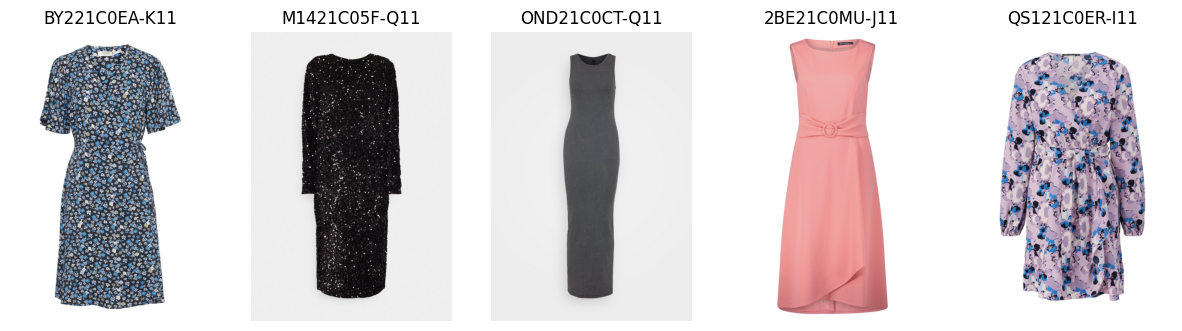
\includegraphics[width=1\linewidth]{Thesis/Dataset/random_sample.png}
    \caption{Random samples from the dataset}
    \label{fig:random_samples}
\end{figure}
\section{Method}
To achieve the goal of this work, the creation of a fine-grained typicality manipulation method, a modular and sequential workflow needs to be designed, which can be seen in figure \ref{fig:method_overview}. A given real image first needs to be inverted using a GAN inversion model (section \ref{sec:method_gan_inversion}) and the corresponding latent code obtained. Using a latent space manipulation technique (section \ref{sec:manipulation}), multiple new latent codes can be found that should exhibit the desired attributes. These latent codes are passed through a custom generator model and thus turned into images for which the typicality scores can be calculated using the custom typicality assessors described in section \ref{sec:typicality_measures}.
\begin{figure}[ht!]
    \centering
    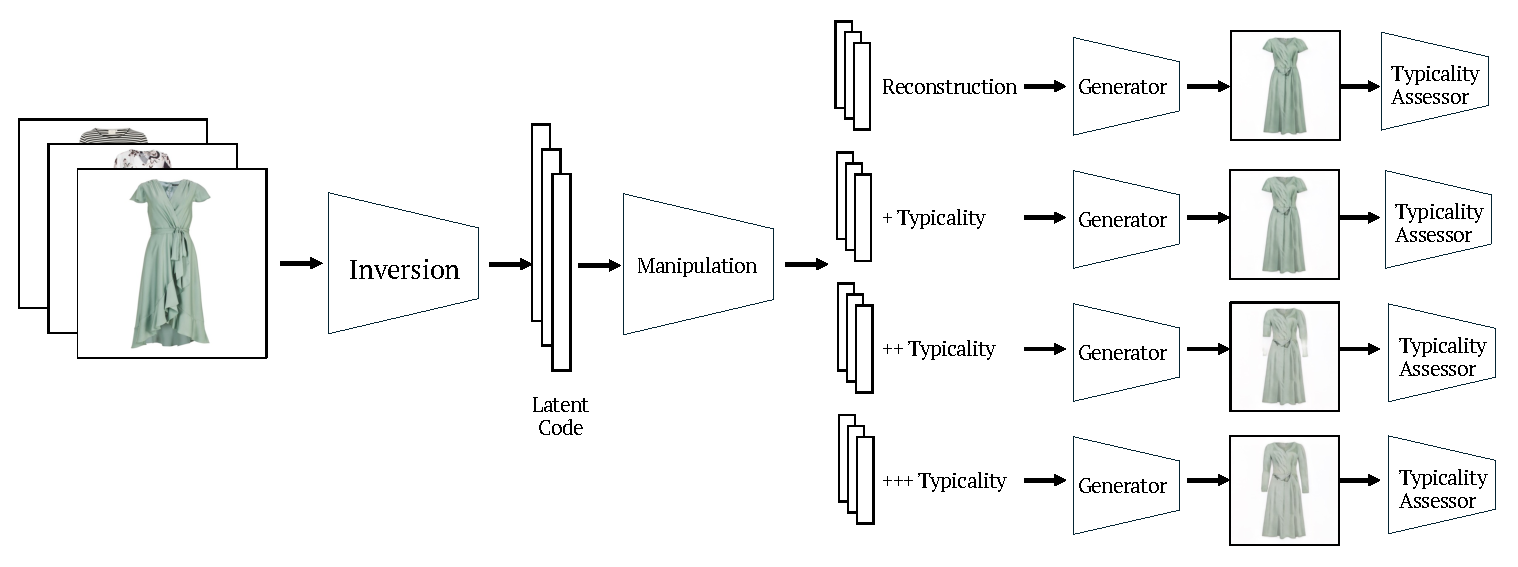
\includegraphics[width=1\linewidth]{Thesis/Method/assets/Method_Overview-cropped.pdf}
    \caption{Inference Workflow}
    \label{fig:method_overview}
\end{figure}
In practice, the order of training the models differs from this inference workflow (see figure \ref{fig:training_pipeline}). As a first step, a generator model needs to be trained which is capable of generating images similar to the distribution of the images one wants to manipulate. This generator model is used in the second step when building an inversion model that achieves good reconstruction and editing performance. As a third step, the typicality assessor is built using the reconstructions of the real images. In the last step, the manipulation model is trained based on the typicality scores and the latent codes from the inversion step.  In the following sections, I will explain the different steps of this process in more detail and explain the methods applied in this work.

\begin{figure}[ht!]
    \centering
    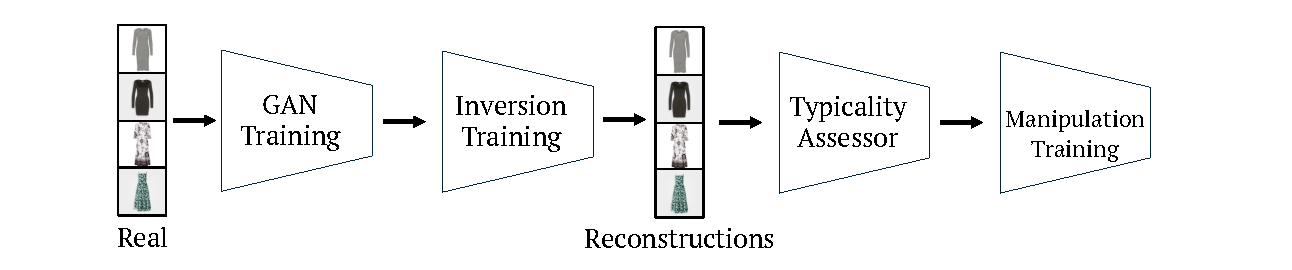
\includegraphics[width=1\linewidth]{Thesis/Method/assets/training_pipeline-cropped.pdf}
    \caption{Training Workflow}
    \label{fig:training_pipeline}
\end{figure}



%%%%%%%%%%%%%%%%%%%%%%%%%%%%%%%
% Dataset 
%%%%%%%%%%%%%%%%%%%%%%%%%%%%%%
\section{Dataset}
All models are trained on a newly created dataset of dresses from Zalando, one of the most popular online fashion retailers in Europe \citep[p.1]{freno2017practical}. The initial dataset consists of article information and image URLs of all publicly available dresses listed on the website "zalando.de" at the time of creation in March 2024. As a first pre-processing step, all articles that do not offer a standardized and centered packshot image of the dress are removed. Afterwards, all images are downloaded, squared in 1024x1024 resolution, and centered. Additionally, the article information is subset to attributes that offer good data completeness and non-noisy labels. The subset consists of the attributes "brand", "price", "category", "fabric", "fit", "neckline", "pattern", "collar", "length", "shape" and "sleeve length". These attributes are cleaned such that similar but small categories are grouped and categories with very few samples are recoded as missing to reduce the dimensionality of each attribute. Since there is no standardized color attribute, the color of each dress is obtained using a pre-trained CLIP model \citep[p.2]{radford2021learning} and a fixed list of 14 colors. The final dataset consists of 14,060 images with the corresponding article information from 643 unique brands. A random sample of images from the dataset can be seen in figure \ref{fig:random_samples}.

\begin{figure}[ht]
    \centering
    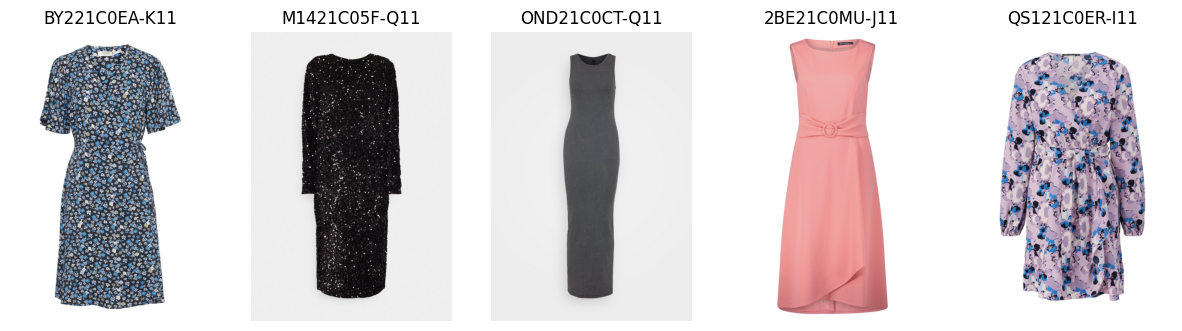
\includegraphics[width=1\linewidth]{Thesis/Dataset/random_sample.png}
    \caption{Random samples from the dataset}
    \label{fig:random_samples}
\end{figure}
% Generation 
%%%%%%%%%%%%%%%%%%%%%%%%%%%%%%
\subsection{Generation}
While multiple GAN-based architectures might be suitable, StyleGAN-based architectures have become the golden standard for image editing \citep[p.1]{bermano2022state}. This is mainly because they learn a highly disentangled and smooth latent space which allows for semantic attribute manipulation (see section \ref{sec:gans}). Within the family of StyleGAN-based architectures, StyleGAN2-Ada \citep{stylegan2ada} is chosen due to its remarkable capabilities to be trained on a small sample. Since the dataset acquired for training is limited by the availability of products on Zalando, training a traditional GAN model is not easily possible. Using StyleGAN2-Ada allows to train a high-fidelity generator even with a dataset of only 14k images.

\subsubsection{Training} \label{sec:sg2_training}
The StyleGAN2-Ada model used in this work has been trained for a resolution of 512x512 pixels per image using the "auto" configuration as defined in \cite{stylegan2ada} and additional x-flip augmentations to increase the dataset size. This configuration uses a reduced depth of the mapping network from 8 to 2 linear layers as this is sufficient according to the authors \citep[Appendix p.35]{stylegan2}. A transfer learning approach from the FFHQ-dataset \citep{stylegan1} is chosen since both datasets rely on centered images with non-relevant backgrounds. Using a pre-trained StyleGAN2-Ada model as the starting point speeds up the training process. The model has been trained for 26 hours on two NVIDIA Tesla V100 GPUs with 32GB VRAM. In total, 2000k images have been shown to the discriminator. Network snapshots have been saved every 40k images shown to the discriminator to later determine the best snapshot using the evaluation metrics described in section \ref{sec:gan_evaluation}.

\subsubsection{Evaluation}\label{sec:gan_evaluation}
The two most widely used GAN evaluation metrics are the Fr\'echet Inception Distance (FID) and the Inception Score (IS) \citep[p.2]{borji2022pros}. The IS \citep{salimans2016improved} evaluates the quality of generated images using ImegNet \citep{deng2009imagenet} predictions from an InceptionV3 \citep{szegedy2016rethinking} model. It combines the confidence of the conditional class predictions (indicating image quality) with the diversity of the predicted classes across the dataset (indicating image diversity). FID \citep{heusel2017gans} on the other hand calculates features of the real and generated datasets using intermediate layers of the same InceptionV3 \citep{szegedy2016rethinking} network and computes the Fr\'echet Inception Distance distance between them. \cite{heusel2017gans} define the FID using multivariate Gaussians over the extracted features as: 
$$\text{FID}(x, g) = \| \bs{\mu_x} - \bs{\mu_g} \|^2 + \text{Tr}\left( \bs{\Sigma_x} + \bs{\Sigma_g} - 2(\bs{\Sigma_x}  \bs{\Sigma_g})^{1/2} \right),$$
where $\bs{\mu_x}$, $\bs{\mu_g}$, $\bs{\Sigma_x} $ and $\bs{\Sigma_g}$ are the mean vectors and covariance matrices of the real and generated image distributions, respectively, and $\text{Tr}$ denotes the trace of a matrix. 

FID is consistent with human inspection and can detect intra-class mode collapse \citep[p.2]{borji2022pros}. As a drawback, for FID to be accurate and comparable, it needs to be calculated on a large and comparable number of samples. Hence, in all my experiments, I calculate the FID based on 50k generated images. As an alternative method, \cite{binkowski2018demystifying} proposed the Kernel Inception Distance (KID) which promises to be an unbiased version of the FID. In practice, there is a very high Spearman rank-order correlation between FID and KID \citep[p.3]{kurach2018gan}. While both the IS and the FID are single-score metrics that evaluate the quality and diversity of generations together, \cite{sajjadi2018assessing} propose improved formulations of precision and recall as GAN evaluation metrics. Recall estimates the fraction of the training set that the generator can reproduce while precision denotes the fraction of generated images that are realistic \citep[p.5]{kynkaanniemi2019improved}. Thus, when training a GAN, one aims for high precision and recall such that the generated images are as realistic as possible while also being as diverse as possible. Naturally, there is a trade-off between the two since a model that can create more diverse generations spans a much larger latent space, thus possibly allowing latent codes from ill-defined regions of this latent space that exhibit less realistic generations. To get a holistic assessment of the generation quality, I calculate all the above-mentioned evaluation metrics and select the best model snapshot based on a comprehensive analysis of the metrics.
%%%%%%%%%%%%%%%%%%%%%%%%%%%%%%
% Inversion 
%%%%%%%%%%%%%%%%%%%%%%%%%%%%%%
\subsection{Inversion}\label{sec:method_gan_inversion}
After a thorough literature review of available inversion methods (see section \ref{sec:gan_inversion}), a set of suitable methods was selected. The baseline model chosen is e4e \citep{tov2021designing} from the encoder-based models. Additionally, three hybrid models are tested: PTI \citep{roich2022pivotal}, ReStyle \citep{alaluf2021restyle}, and Hyperstyle \citep{alaluf2022hyperstyle}. Among these, PTI promises the best inversion performance but with a high inference time. To reduce inference time, ReStyle and Hyperstyle were selected as they promise similar results to PTI at a fraction of the time.

% After conducting a thorough literature research on available inversion methods (see section \ref{sec:gan_inversion}), a set of suitable methods has been selected. Since optimization-based methods have a prohibitively slow inference time and low editability performance \citep[p.3]{tov2021designing}, no pure optimization-based method has been selected. As a baseline inversion method, encoder4editing (e4e) \citep{tov2021designing} has been selected. This method promises high reconstruction quality while being specifically optimized to produce highly editable latent codes. Additionally, e4e is an encoder-based method and thus has a very fast inference time which allows to obtain latent codes for the complete dataset in a reasonable amount of time. Furthermore, many other inversion methods rely on e4e inversions as initial latent codes in their optimization. Using e4e, inversions into $\mathcal{W}^+$-space are obtained. The authors claim that there is a trade-off between distortion and editability when inverting into $\mathcal{W}$ or $\mathcal{W}^+$-space. While inversion into $\mathcal{W}^+$ leads to better reconstructions, it may come at the cost of editability \citep[p.5]{tov2021designing}. Encoder4editing for designed to specifically mitigate this, therefore in this work, only inversions into $\mathcal{W}^+$-space are used. From the domain of hybrid models, PTI \citep{roich2022pivotal} has been selected due to its proven state-of-the-art inversion performance \citep[p.1]{roich2022pivotal}. PTI builds upon e4e and uses its latent code as a starting point. It then pivots the generator weights such that the reconstruction quality increases. Since the latent code of the inversion is still the simple e4e inversion, it still lies in the editable region of the latent space, but thanks to the slightly changed generator, achieves much better reconstruction. Since the generator weights have to be optimized for each sample individually, inference time is very high. Therefore, two additional models have been tested which promise similar inversion performance at a fraction of the inference time. ReStyle \citep{alaluf2021restyle} and Hyperstyle \citep{alaluf2022hyperstyle} are models that again build upon e4e. ReStyle learns iterative refinement steps of the original e4e latent code by learning residual weights. Hyperstyle on the other hand builds upon ReStyle latent codes and additionally learns hyper-network weights for the convolutional filters of the generator. While this also changes the generator weights as in PTI, the hyper-network is learned during training and does not need to be optimized for every sample. Thus, inference time is drastically reduced.

\subsubsection{Training}
For training of the e4e model, the dataset has been randomly split into 90\% training samples and 10\% test samples. The model was trained with default parameters as defined in \cite{tov2021designing} and checkpoints were saved every 2000 steps.  In total, the model has been trained for 38 hours on one GPU. As can be seen in the loss curves for the overall loss, the LPIPS loss, and the L2 loss in figure \ref{fig:e4e_loss_curves}, the model has converged within this time. ReStyle and Hyperstyle have been trained with default parameters. ReStyle has initially been trained for 35 hours on one GPU but had not converged yet. Therefore it was trained for another 20 hours, totaling 55 hours of training time. Hyperstyle was trained for 40 hours and an additional 30 hours until convergence, totaling 70 hours of training time on one GPU. For all models, NVIDIA Tesla V100 GPUs with 32GB of VRAM were used.




\subsubsection{Evaluation}
Evaluating GAN inversion involves multiple dimensions. Generally, evaluation metrics can be grouped into three dimensions: Faithfulness (i.e. reconstruction quality), photorealism (i.e. perceptual quality),  and editability of the latent code \citep[p.3]{xia2022gan}. \\
Faithfulness measures the quality of the reconstruction, i.e. how closely the generated image from the inversion resembles the real image. One of the early measures proposed was Peak signal-to-noise ratio (PSNR). Many works additionally consider the Structural Similarity Index (SSIM) \citep{wang2004image} which measures the similarity using three key features: Luminance, Contrast, and Structure \cite[p.6]{wang2004image}. It has been shown that SSIM more closely correlates with human perception than PSNR \cite[p.19]{sheikh2006statistical}. For my evaluation, I use the advanced version of SSIM, the Multi Scale Structural Similarity Index Measures (MSSSIM) proposed by \cite{wang2003multiscale}.  Furthermore, multiple pixel-wise distances (e.g. mean squared error, mean absolute error) have been proposed. Since close reconstruction of input images is important in this work, the pixel-wise $\mathcal{L}_2$ distance will be used as an additional measure of faithfulness. \\
Measuring the perceptual quality of images (i.e. photorealism) against a reference dataset is described in chapter \ref{sec:gan_evaluation} in more detail. Many works rely on the same measures to evaluate the quality of the inversion process. I use the FID \citep{heusel2017gans} to measure how close the generated images from the inversions resemble the distribution of the real data. Furthermore, I use Learned Perceptual Image Patch Similarity (LPIPS) proposed by \cite{zhang2018unreasonable} which measures similarity between two images using features extracted from a VGG model \citep{simonyan2014very} trained on ImageNet \citep{deng2009imagenet}. \\
While the first two dimensions can be directly measured using multiple metrics, the editability of the latent code from an inversion method is not easily tested. Evaluating the editability involves yet another model, the editing technique. Thus, the evaluation of this dimension is very closely connected to the evaluation of the manipulation technique described in section \ref{sec:manipulation}. If the manipulation is not successful, it is difficult to find out whether the latent code itself is not editable or whether the manipulation method for the attribute does not work. As a qualitative measure for editing capabilities of inversions, \cite{zhu2020improved} propose to evaluate the quality of images generated from interpolating between two latent codes. They argue that an inversion is good if the interpolated images are of high quality \citep[p.10]{zhu2020improved}. In general, preserving the original identity during edits and only editing localized attributes is of high importance. \cite{alaluf2021only} and \cite{richardson2021encoding} use facial recognition networks as proposed in \citep{deng2019arcface} to assess identity preservation via cosine similarity of facial identity representations. For non-facial data, using this technique is challenging since training identity recognition networks for other domains is difficult \citep[p.13]{bermano2022state}. As \cite{tov2021designing} point out, all popular quantitative metrics to evaluate editing performance contradict each other and often the human judgment \citep[p.7]{tov2021designing}. \\
Given the difficulty of evaluating the editing capabilities of inversion methods, I focus on quantitative metrics for faithfulness and photorealism when comparing the different inversion methods. To assess the editing capabilities of the latent codes, I rely on interpolation experiments as proposed by \citep{zhu2020improved} and eventually on the results obtained from the downstream manipulation method.
\subsection{Typicality Measures}\label{sec:typicality_measures}
Measuring typicality, i.e. how "dressy" a dress looks like, is a central aspect of the overall workflow. Having a consistent typicality measure allows to create supervision needed in the training of the manipulation method. Furthermore, it allows to validate the success of the manipulation ex-post quantitatively. Based on work by \cite{landwehr2011gut}, typicality is measured based on the cosine similarity of a product's features (i.e. its embedding) to a morph of the features of all products. With $f(\cdot)$ being any embedding model, the d-dimensional embedding for dress $D_i$ is calculated as $\boldsymbol{v}_i = f(D_i)$. Furthermore, the morph of all dresses is 
$$\boldsymbol{m} = \frac{1}{n} \sum_{i=1}^{n}\boldsymbol{v}_i,$$
with $\boldsymbol{v}_i \in \mathbb{R}^d$ and $\boldsymbol{m} \in \mathbb{R}^d$. Finally, the typicality measure for dress $D_i$ is 
$$typicality = cosine\_similarity(\boldsymbol{v}_i, \boldsymbol{m}) = \frac{\boldsymbol{v}_i \cdot \boldsymbol{m}}{|\boldsymbol{v}_i||\boldsymbol{m}|}.$$
In the first step, as a simple embedding model the pre-trained Vision Transformer (ViT) DINOv2 \citep{oquab2023dinov2} is used. More specifically, the "Base" version is used with a patch size of 14, i.e. the "ViT-B/14" configuration. The resulting embeddings are 1x768 dimensional. The authors claim that the representations are task-agnostic and general-purpose \citep[p.1]{oquab2023dinov2} and thus can be used for typicality analysis. While this approach may overfit to non-essential attributes or use shortcuts, the second embedding model I use aims to produce more holistic and robust representations. It does so by forcing the embedding model to learn multiple sub-embeddings, one for each relevant attribute of the dress. Thus, the decision about which features or attributes are important to represent a dress is not exclusively taken by the model as in the pure DINOv2 case but is defined ex-ante based on domain knowledge. The model starts with the simple DINOv2 embeddings and passes them through some fully connected layers. Afterwards, the embedding is split up into k subspaces $a_1,a_2,...,a_k$ by individual classification heads $C_1,C_2,...,C_k$, one for each attribute. The attributes selected consist of \textit{Color, Fabric, Fit, Neckline, Pattern, Collar, Length, Shape} and \textit{Sleeve Length}. Since the goal is to achieve disentangled sub-embeddings, a distance correlation (dCor) loss is added to the model training, enforcing the reduction of shared information across sub-embeddings. The distance correlation proposed by \cite{muller2024disentangling} measures nonlinear dependencies between vectors of any dimension and has been used by the authors for disentangled representation learning. The dCor loss is defined as 
$$\mathcal{L}_{dCor} = \sum_{i \neq j} \text{dCor}(a_i, a_j),$$
with 
$$\text{dCor}(a_1, a_2) = \sqrt{\frac{\text{dCov}^2(a_1, a_2)}{(\text{dVar}^2(a_1) \text{dVar}^2(a_2))^{1/2}}}.$$
Details about calculating $\text{dCov}^2$ and $\text{dVar}^2$ can be found in the original paper \citep[p.5]{muller2024disentangling} and in the appendix in equation \ref{eq:dcor_formula} to \ref{eq:last_dcor_formula}. A schematic overview of the disentangled embeddings model can be found in figure \ref{fig:disentangling_embeddings}.

\begin{figure}[ht!]
    \centering
    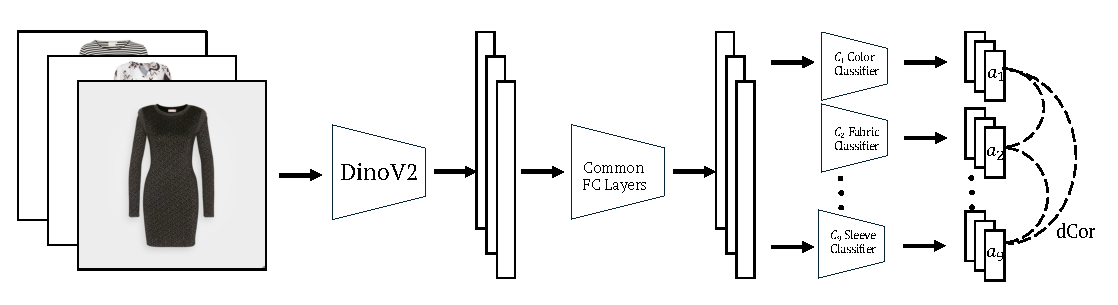
\includegraphics[width=1\linewidth]{Thesis/Method/assets/disentangling_embeddings-cropped.pdf}
    \caption[Disentangled Embeddings Model for Typicality]{Disentangled Embeddings Model for Typicality: \textit{Initial DINOv2 embeddings are divided into subspace embeddings $a_1,a_2,...,a_k$ by classifiers. Disentanglement is forced by a distance correlation loss between all sub-embeddings}}
    \label{fig:disentangling_embeddings}
\end{figure}

Each subspace embedding in this disentangled embedding model is 1x256 dimensional and thus the complete embedding, which is a concatenation of all subspace embeddings, has dimension 1x2304. Apart from the complete concatenation, I also construct embeddings that exclude one subspace at a time. This might be e.g. all subspace embeddings except the \textit{Color} subspace such that the model can calculate the typicality of a dress but does not take the \textit{Color} attribute of the dress into account.


It is important to note that both typicality measures are learned on the reconstructed images using the e4e inversion \citep{tov2021designing}. Thus, the embeddings for each dress, as well as the morphs, are calculated based on the respective reconstructions. Training the typicality measure on real images and using generated images at test time holds potential for problems. Although the reconstructions are very accurate, pixel values and low-level image features might differ between the generator outputs and the real image distribution, thus introducing possible mismatches in the typicality calculations.
%%%%%%%%%%%%%%%%%%%%%%%%%%%%%%
% Manipulation 
%%%%%%%%%%%%%%%%%%%%%%%%%%%%%%
\subsection{Manipulation}\label{sec:manipulation}
As mentioned before, I tested a linear (\textit{InterFaceGAN)} and a non-linear (\textit{StyleFlow}) approach, both from the family of supervised latent space manipulation techniques. Due to its low editing performance and prohibitively high computational cost, \textit{StyleFlow} has been disregarded after initial editing experiments on physical attributes like color or sleeve length of a dress. \textit{InterFaceGAN} on the other hand was used throughout all experiments in this work.

\subsubsection{InterFaceGAN}\label{sec:interfacegan}
The latent space of StyleGAN models is smoothly interpolable \citep[p.1]{stylegan1} and gradual changes in one direction in the latent space of a well-trained generator can result in gradual changes in a specific semantic attribute \citep[p.6]{bermano2022state}. \cite{shen2020interpreting} propose a simple, yet effective method of finding this direction in a method called \textit{InterFaceGAN}. The method is based on the assumption that for any binary semantic, a hyperplane in the latent space can be found that separates the two classes \citep[p.3]{shen2020interpreting}. Assuming a hyperplane with a unit normal vector $\mathbf{n} \in \mathbb{R}^d$, with $d$ being the dimension of the latent space, the "distance" of the latent representation of sample $\mathbf{z}$ to the hyperplane can be defined as 
\[d(\mathbf{n, z}) = \mathbf{n}^T\mathbf{z}.\]
If one moves towards and across the hyperplane in the latent space, the sign of the distance changes, and thus the semantic attribute in the generated image should have changed to the opposite class \citep[p.3]{shen2020interpreting}. 

\begin{wrapfigure}{r}{6cm}
    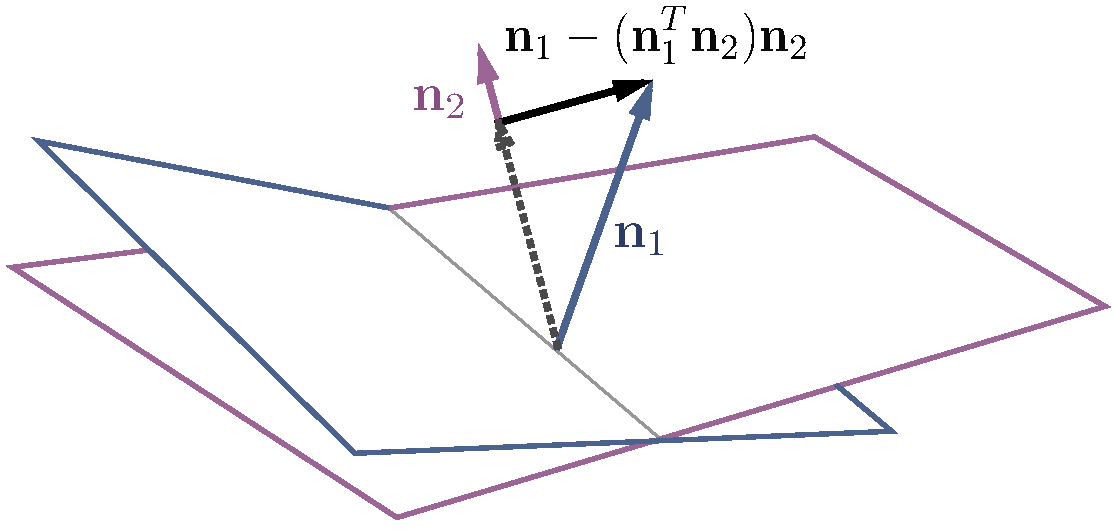
\includegraphics[width=6cm]{Thesis/Method/assets/subspace_projection.pdf}
    \caption[Conditional manipulation via subspace projection]{Conditional manipulation via subspace projection - taken from \cite{shen2020interpreting}, p.4}
    \label{fig:subspace_projection}
\end{wrapfigure} 

While this is straightforward for a single binary attribute, often multiple semantics are present and might not be independent of each other, although the latent space of StyleGAN models already enforces some degree of disentanglement (see section \ref{sec:gans}). In the case of $m$ semantics, $m$ separation boundaries $\mathbf{N} = [\mathbf{n_1, ..., n_m}]$ can be found. To disentangle them, $\{\mathbf{n_1, ..., n_m}\}$ need to be orthogonal to each other \citep[p.4]{shen2020interpreting}. In practice, conditional manipulation, i.e. editing one semantic without affecting any other semantic, can be performed using projection. As illustrated in figure \ref{fig:subspace_projection}, if one wants to manipulate the semantic connected with the hyperplane $\mathbf{n_1}$ without affecting the semantic connected with $\mathbf{n_2}$, the projection of  $\mathbf{n_1}$ onto $\mathbf{n_2}$ is subtracted from $\mathbf{n_1}$. Thus, the conditional manipulation direction is
$$\mathbf{n_{cond}} = \mathbf{n_1} - (\mathbf{n_1}^T\mathbf{n_2})\mathbf{n_2}.$$
For the semantic editing, the authors apply a simple linear manipulation of the latent space in the positive or negative direction of the unit normal vector $\mathbf{n}$ of the separation boundary. Thus the manipulated latent representation is defined as
$$\mathbf{z}_{edit} = \mathbf{z} + \alpha\mathbf{n},$$
with the synthesis being more positive on the semantic for $\alpha >0$ and more negative with $\alpha <0$ \citep[p.4]{shen2020interpreting}.

Since \textit{InterFaceGAN} is a supervised approach, either labels for the semantics or classifier scores need to be available. If there are labels available, those can directly be used to find a hyperplane that separates the latent space based on these labels. If only classifier scores are available, the authors propose to use the samples with the highest and lowest scores and assign binary labels. The hyperplane is then found by training a simple linear classifier on the latent representations. In this case, a linear Support Vector Machine (SVM) is trained. Linear SVMs learn a decision boundary which acts as the separation boundary in latent space that is used by InterFaceGAN.

\subsubsection{Training}\label{sec:interfacegan_training}

To make the \textit{InterFaceGAN} approach usable for this work, some implementation details needed to be adapted. While the authors used the 512-dimensional $\mathcal{Z}$-space of StyleGAN, I used the 16x512-dimensional $\mathcal{W^+}$-space. Thus, finding a hyperplane in this higher dimensional space is not as straightforward as in $\mathcal{Z}$. To tackle this problem, one could either flatten the latent representation in $\mathcal{W^+}$-space by concatenating all 16 dimensions along one dimension or learn 16 separate hyperplanes, one for each of the dimensions. The latter results in individual manipulations in each of the 16 dimensions. As explained in section \ref{sec:gans}, the various dimensions of $\mathcal{W}$ and $\mathcal{W^+}$ are injected at different levels of the synthesis process and allow targeted variations at different scopes of the image. Thus, learning isolated separation boundaries allows to apply targeted manipulation in the specific semantic only at a certain coarseness level of the generation process. On the other hand, learning one separation boundary from the complete latent representation allows the linear classifier to consider all features at all levels at the same time when finding the manipulation direction. Both approaches have been implemented and tested and the results are very similar. Since the isolated boundaries approach requires another step of selecting the dimensions to consider in the manipulation, the method of flattening the latent space has been selected as the final approach, thus simplifying the process without sacrificing editing performance. \\
When constructing the training data for the typicality scores, I closely follow the authors of \textit{InterFaceGAN} by using only the top $n$ and bottom $n$ scores in the classifier training. The idea is to create two distinct classes that can be clearly separated and that exhibit strong attributes of the two classes, i.e. high and low typicality. The boundaries have been computed using values of $n=1000$, $n=2000$, and $n=3000$. Finally, the separation accuracy on a separate validation set has been computed and the boundary with the best accuracy was selected as the final manipulation direction. \\
Another difference in the \textit{InterFaceGAN} implementation between this work and the original approach is the nature of the semantics. While the authors could show that the approach works well on naturally binary attributes like gender or the presence of glasses in facial images, or ordinal features like the age of a person, the labels present in the dresses dataset are different. Physical attributes like color or sleeve length, which are used as conditioning factors in the typicality manipulation, are nominal and have high cardinality. For those attributes, $\frac{n!}{2!(n-2)!}$ hyperplanes are calculated with $n$ being the number of unique values an attribute has. Therefore, there are hyperplanes for each combination of binary directions in the feature space. Defining one attribute value as positive while assigning all the others to the negative class (one-vs-rest) leads to multiple problems. First of all, the linear classification problem becomes extremely imbalanced. Furthermore, according to \cite{yang2021discovering} that set of negative samples provides ambiguous or even misleading guidance to the linear classifier, resulting in entangled semantics and incorrect manipulation directions \citep[p.1]{yang2021discovering}. When choosing a specific boundary as the conditional boundary, the set of boundaries to choose from is restricted to those that cover the real attribute value. So if the conditioning is on the color attribute and the dress is blue, all boundaries that include "blue" together with any other color are candidates. Out of the candidates, the boundary that has the best accuracy on the validation set during the classifier training is chosen. To visually validate the quality of these physical attribute boundaries, some preliminary manipulation tests using physical attributes have been run. The results of these experiments can be found in the appendix in figure \ref{fig:physical_attributes_manipulation}. Furthermore, descriptive statistics for the multiple separation performances of the physical attributes can be found in table \ref{tab:physical_summary_stats} in the appendix.





\section{Results}\label{sec:results}

\subsection{Generator Training}
To evaluate the performance of the StyleGAN2-Ada generator, multiple evaluation metrics have been computed for different snapshots saved during training. Training curves for the StyleGAN2-Ada model can be found in the appendix in figure \ref{fig:sg2ada_evaluation_metrics}. FID and KID are at the lowest at step 1200, meaning after 1200k images have been shown to the discriminator. Interestingly, IS shows the highest value at step 1800. Since the value at step 1200 is also fairly high and IS is less meaningful for the task at hand as described in section \ref{sec:gan_evaluation}, this discrepancy is ignored. Looking at the Precision and Recall curves, Precision, i.e. the fraction of realistic-looking images peaks early at step 600 while Recall, i.e. the diversity of generated images peaks at step 1200. Since there is an inherent trade-off between the two, I choose higher diversity while accepting a slightly lower fidelity in the generations. Consequently, step 1200 is chosen as the model to be used in all downstream applications.
\begin{figure}[ht!]
    \centering
    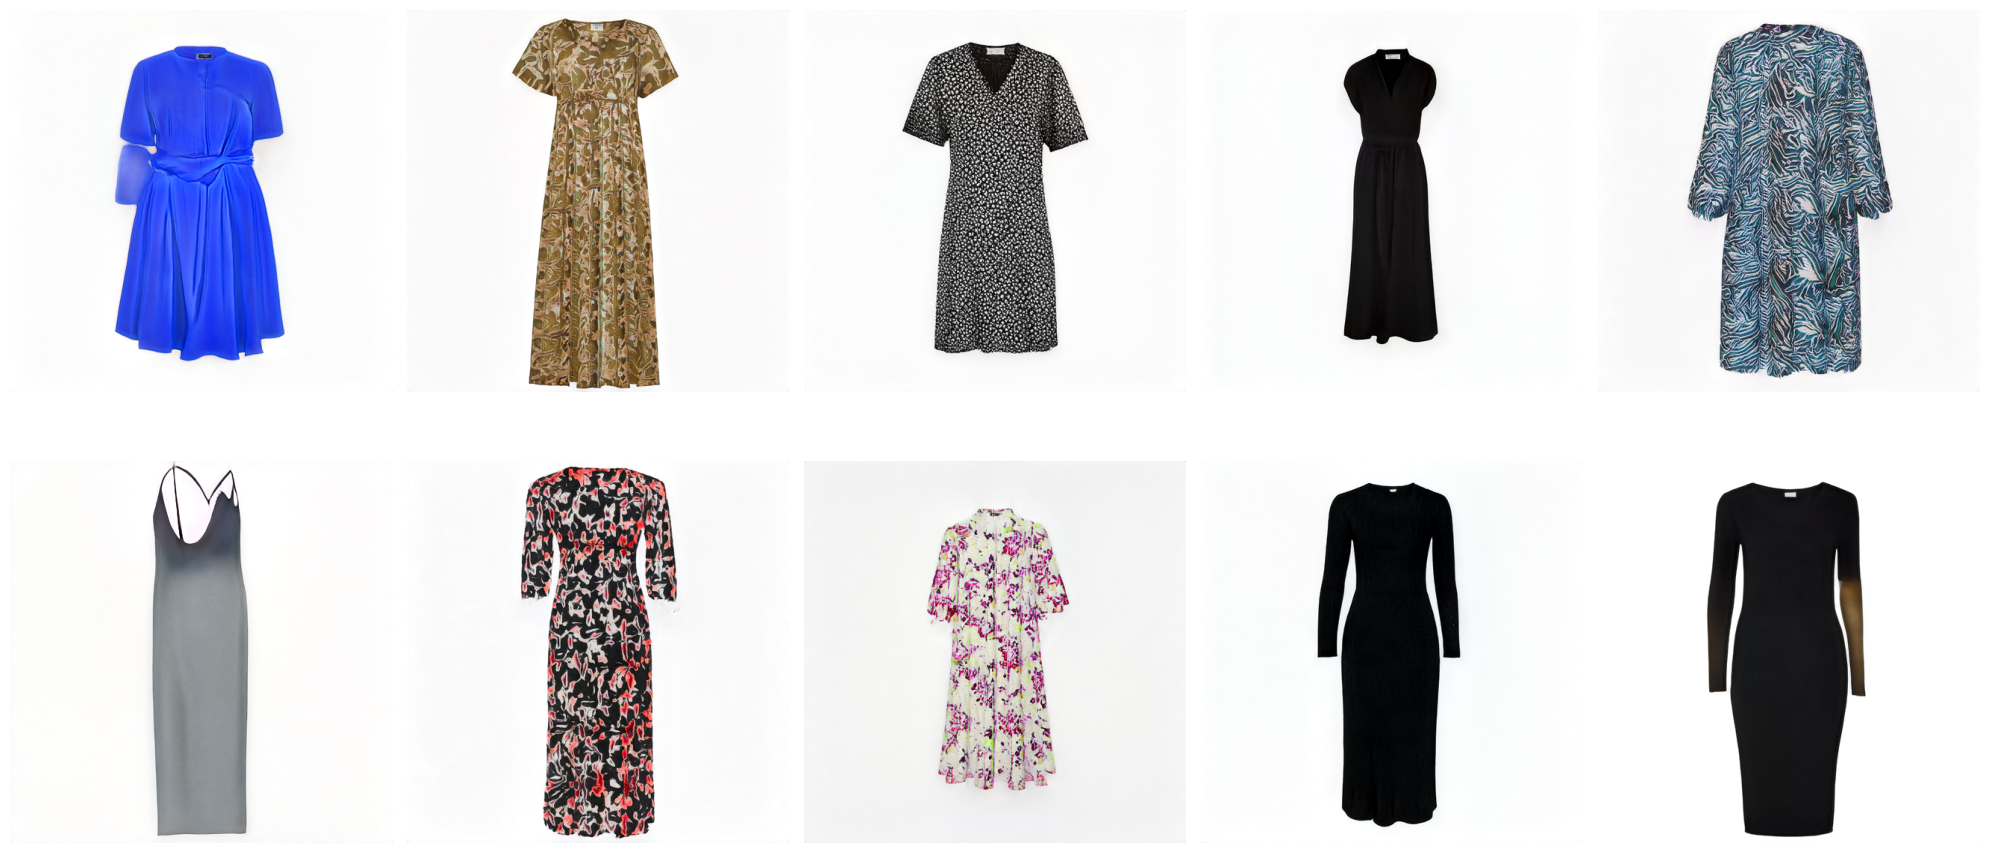
\includegraphics[width=1\linewidth]{Thesis/Results/assets/generated_samples.png}
    \caption[Generated Dresses from StyleGAN2-Ada Model]{Generated Dresses from StyleGAN2-Ada Model \textit{The random generation showcases the diversity of dresses that the generator is capable of generating. At the same time, some generations may exhibit artifacts like the two different sleeve lengths in the upper left image.}}
    \label{fig:generated_samples}
\end{figure}

To validate the training results, both a quantitative evaluation against comparable models in literature as well as a qualitative evaluation are conducted. With a final FID score of 8.09, the generator performance lies exactly in the range of 7.5-10.0 which has been established in the original StyleGAN2-Ada paper for datasets with comparable sizes \citep[p.8]{stylegan2}. Other applications of StyleGAN2-Ada have similar FID scores (e.g. 8.7 in \cite{fu2022stylegan}) or much higher scores (e.g. 13.68 in \cite{hermosilla2021thermal} and 26.02 in \cite{kim2022effective}). A similar application that aims at clothing generation could achieve an FID of 4.53 using a conditional StyleGAN2-Ada model and training on a much larger dataset of 62k images for ten days. Given those benchmark results, the FID achieved for my StyleGAN2-Ada model is well in the range of applications with similar dataset sizes and computational resources used. For a qualitative evaluation of the images generated by the final model, please refer to figure \ref{fig:generated_samples}.



\subsection{Inversion}
In general, all inversion models implemented (e4e, ReStyle, Hyperstyle, PTI) achieve relatively good reconstruction quality as can be seen in figure \ref{fig:inversion_results}. It becomes clear that even the encoder-based method e4e can relatively well reconstruct the original images. There are however some finer details missing in the e4e inversions that the more advanced models can capture. Looking at the samples in figure \ref{fig:inversion_results}, one can see that the e4e model struggles with very fine fabric details as shown in the mesh fabric in the first and last row, and with more complex patterns as in the third and fourth row. The other methods seem to be able to capture those details, while it becomes clear that PTI seems most successful at reconstructing the dress with all details, especially the complex patterns. The results of the qualitative evaluation from figure \ref{fig:inversion_results} are also in line with the quantitative results in table \ref{tab:inversion_metrics}. Here, e4e shows the highest LPIPS and L2 scores while having the lowest MSSSIM results. Interestingly, the reconstructions show a higher FID score than the random generations obtained from the StyleGAN2-Ada model. This is also the case for ReStyle, although all other metrics show Restyle as better performing than e4e. Hyperstyle performs strictly better than both e4e and Restyle based on these metrics. This is also obvious when looking a the reconstructions in figure \ref{fig:inversion_results}. For PTI inversions, FID could not be calculated, as the model was run only for 500 dresses, which is not enough for FID calculations. The reason for the small sample size is the high inference time of 1.3 minutes per instance. The other metrics however can easily be calculated for PTI, since they are based on direct comparison of originals and reconstructions, regardless of the sample size. PTI shows superior performance in all metrics against Hyperstyle. The LPIPS score of PTI is almost half the magnitude as for Hyperstyle, indicating a considerable increase in reconstruction quality. This is also in line with the qualitative results from figure \ref{fig:inversion_results}.
\begin{figure}[ht!]
    \centering
    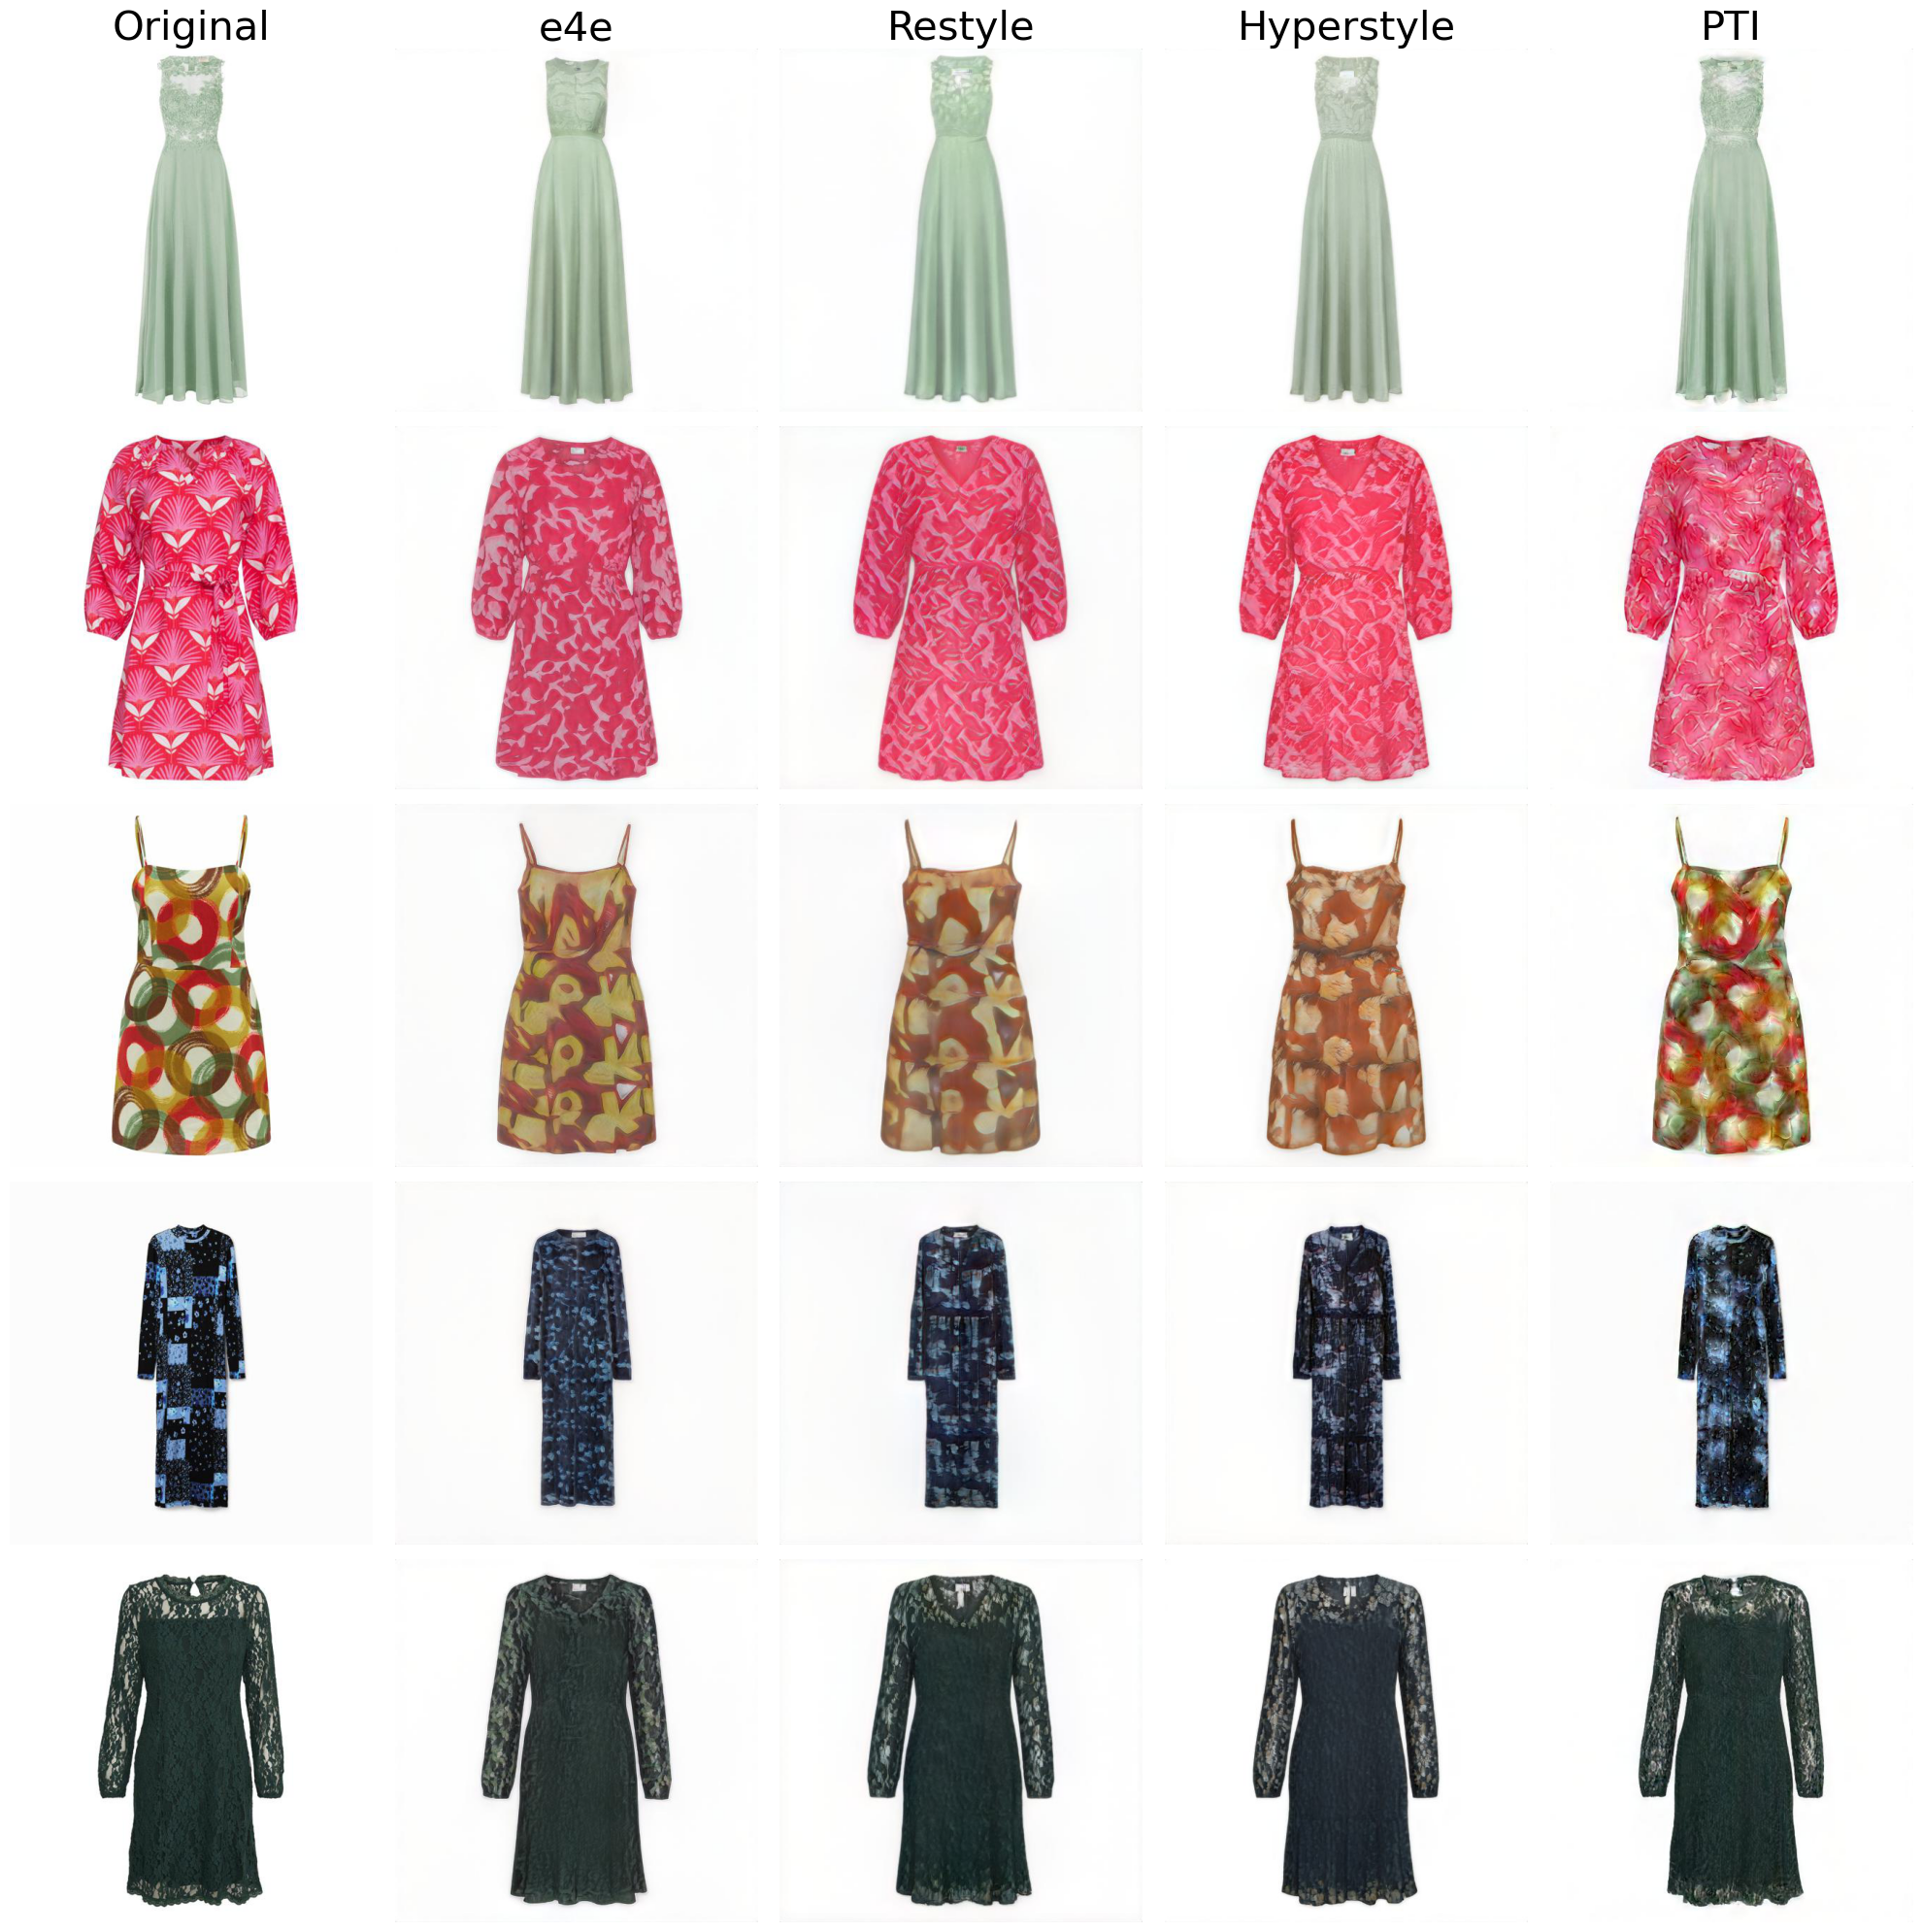
\includegraphics[width=1\linewidth]{Thesis/Results/assets/inversion_results.png}
    \caption[Qualitative Evaluation of Inversion Methods]{Qualitative Evaluation of Inversion Methods: \textit{First column shows the original image, second to last columns show the inversions obtained by various GAN-inversion methods}}
    \label{fig:inversion_results}
\end{figure}
\begin{table}[ht!]
    \centering
    \begin{tabular}{|c|c|c|c|c|c|}
        \hline
          Metric  &   StyleGAN2-Ada &       e4e &   Restyle &   Hyperstyle &    PTI \\
        \hline
        FID    &          8.0966 & 8.13   &    8.4276 &       7.1874 & -      \\
        \hline
         LPIPS  &        -      & 0.114  &    0.1138 &       0.0988 &   0.0502 \\
         \hline
         L2     &        -      & 0.0203 &    0.0147 &       0.0128 &   0.0085 \\
         \hline
         MSSSIM &        -      & 0.8702 &    0.8919 &       0.9053 &   0.945  \\
        \hline
    \end{tabular}
    \caption{Quantitative Evaluation of Inversion Methods}
    \label{tab:inversion_metrics}
\end{table}

\subsection{Typicality Measure}\label{sec:results_typicality_measure}
Looking at samples with the highest and lowest typicality scores for both typicality measures in figure \ref{fig:examples_dino_typicality} and \ref{fig:examples_disentangled_typicality}, it becomes clear that both measures are consistent. A typicality measure is consistent, if the samples that show a high (low) typicality are highly similar in their attributes while they are highly dissimilar to the sample with low (high) typicality scores. For the typicality measure based on DINOv2 embeddings, the highly typical samples have variation in color and sleeve lengths but the neckline and the overall shape of the dress are very similar. In the non-typical dresses, there are mostly very untypical dress shapes. In the typicality measure based on disentangled embeddings, the variation between the most typical dresses seems higher at first glance which is expected, since this is a simple combination of multiple disentangled attribute embeddings. One attribute that seems dominant however is the sleeve length, since the most typical dresses all show long sleeves while the least typical dresses are all sleeveless. If one excludes the attribute sleeve length, the most typical dresses show a waist-fitted shape as can be seen in figure \ref{fig:examples_disentangled_ex_sleevel_length} with varying sleeve lengths. Overall, the typicality measure based on the disentangled embeddings does not allow simple explanations like the one for the DINOv2-based measure, since the exact attributes, that determine that a dress is very typical can vary from dress to dress. 


\subsection{Manipulation}
\subsubsection{Preliminary Experiments}
To test the overall suitability of inversion methods with the InterFaceGAN manipulation scheme, preliminary experiments are run on e4e-, Hyperstyle-, and PTI-inversions. In those experiments, easy-to-manipulate physical attributes like sleeve length or color are manipulated and the overall manipulation performance is visually assessed. Only inversion methods that perform sufficiently well on physical attributes will be considered for the experiments on aesthetic attribute manipulation.
While these manipulations are reliably done for e4e- and PTI-inversions (see figure \ref{fig:physical_attributes_manipulation}), Hyperstyle inversions have a slightly worse manipulation performance. Although manipulation of the physical attributes works for most samples, some samples exhibit faulty artifacts as can be seen in figure \ref{fig:hyperstyle_manipulation_tests}. The reason for this behavior lies in the structure of the Hyperstyle inversions. For Hyperstyle, the latent space of the inversion is only one component of the inversion model. The other component is the weights of the hyper-network which allow Hyperstyle to achieve this superior performance against Restyle and e4e. InterFaceGAN on the other hand operates exclusively on the latent space and incorporating the weights of the hyper-network in this technique is not possible. Since the reliance on the hyper-network weights for my custom Hyperstyle model is too high, the information contained in the latent codes alone is not sufficient to achieve similar manipulation performance as for e4e latents or PTI inversions. Interestingly, PTI also relies on fine-tuned generator weights to produce accurate inversions but achieves much better manipulation performance in the preliminary experiments. The latent codes that build the basis for PTI are the simple e4e latent codes. Therefore, they contain all the semantic information needed to find manipulation directions but can simultaneously be improved by pivoted generator weights from PTI. Therefore, PTI inversions work better with InterFaceGAN than Hyperstyle inversions. Due to Hyperstyle's slightly less reliable manipulation performance in these preliminary tests, and the fact that it was outperformed by PTI in all inversion metrics, Hyperstyle was not considered for further experiments downstream. Consequently, all manipulation experiments below were carried out for e4e inversions using the basic StyleGAN2-Ada generator and PTI inversions using the pivoted generator architectures.

\subsubsection{Selection of InterFaceGAN Boundary}
As described in section \ref{sec:interfacegan_training}, the dataset to train InterFaceGAN for typicality manipulation was created using the top and bottom $n$ samples according to the typicality score. To make manipulation results comparable between all typicality measurements, $n$ is fixed for all embedding types that are used for typicality score calculations. Besides the simple DINOv2 embeddings and the complete disentangled embeddings, InterFaceGAN boundaries were calculated for typicality scores based on disentangled embeddings excluding color and sleeve length attributes. These are used for conditional typicality manipulations. 

\begin{table}[ht]
\centering
\begin{tabular}{|c|c|c|c|c|}
\hline
    &
    \bfseries Simple Embeddings &
    \multicolumn{3}{c|}{\bfseries Disentangled Embeddings}\\
\hline
n & DINOv2 & All & Excl. color & Excl. sleeve length \\ \hline
 1000 &   0.9817 & 1      &        0.9967 &                0.9733 \\
 2000 &   0.9825 & 0.9933 &        0.9967 &                0.9642 \\
 3000 &   0.9522 & 0.9967 &        0.9978 &                0.9394 \\
 \hline
\end{tabular}
\caption[Validation Accuracy of InterfaceGAN Boundaries]{Validation Accuracy of InterfaceGAN Boundaries}
\label{tab:typicality_accuracy}
\end{table}

As can be seen in table \ref{tab:typicality_accuracy}, the validation accuracy for the complete disentangled embeddings and the disentangled embeddings excluding sleeve length is highest for $n=1000$. For the simple DINOv2 embeddings, validation accuracy is highest for $n=2000$  but only slightly lower for $n=1000$. For the disentangled embeddings excluding color, $n=3000$ is optimal, but also only slightly higher than for $n=1000$. Therefore, $n=1000$ is selected for all boundary calculations in the InterFaceGAN methodology. In general, all boundaries achieve very high separation accuracy. Although this is not very surprising, given the training is performed only on the top and bottom $n$ samples, this still indicates that the learned boundary can sensibly separate the two classes.

\FloatBarrier
\subsubsection{Typicality Manipulation}
\begin{figure}[!ht]
    \centering
    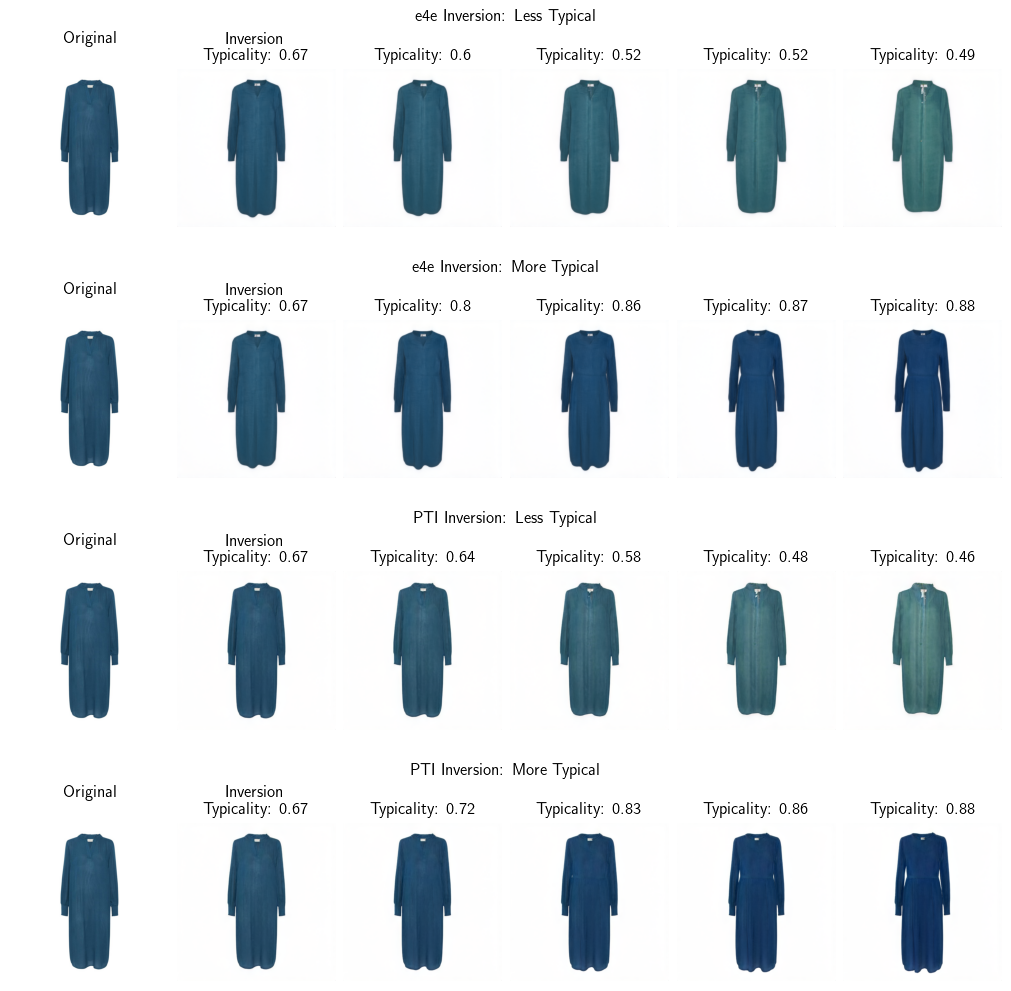
\includegraphics[width=1\linewidth]{Thesis/Results/assets/dino_main_results.png}
    \caption[Typicality Manipulations using DINOv2 Embeddings]{Typicality Manipulations using DINOv2 Embeddings}
    \label{fig:dino_main_results}
\end{figure}

\begin{figure}[!ht]
    \centering
    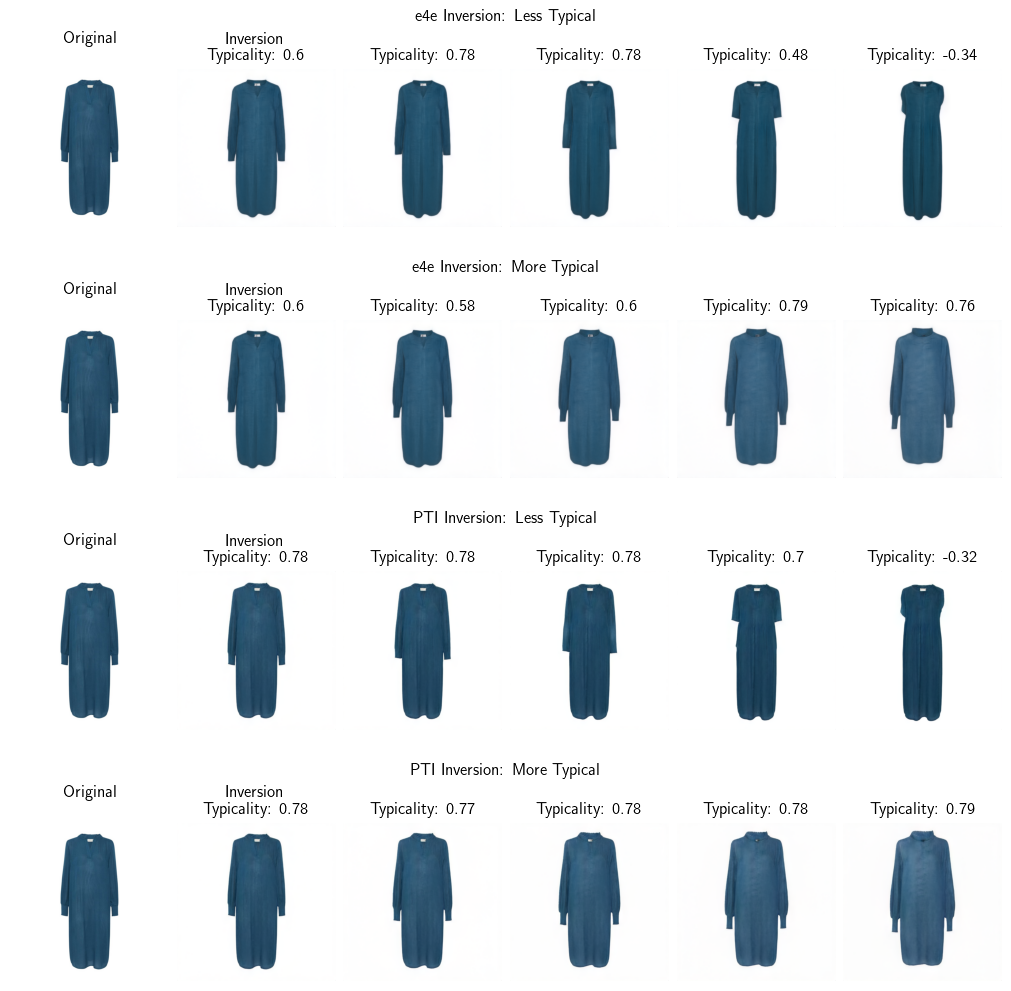
\includegraphics[width=1\linewidth]{Thesis/Results/assets/disentangled_main_results.png}
    \caption[Typicality Manipulations using Disentangled Embeddings]{Typicality Manipulations using Disentangled Embeddings}
    \label{fig:disentangled_main_results}
\end{figure}

For the final typicality manipulation, I compare the two typicality measures against each other, i.e. typicality based on simple DINOv2 embeddings against typicality based on disentangled embeddings. For both embedding types, only e4e and PTI inversions are considered, since those performed well enough in the preliminary experiments. The results of the typicality manipulation based on DINOv2 embeddings and disentangled embeddings for one article (SKU: KA321C13K-K11) are shown in figure \ref{fig:dino_main_results} and \ref{fig:disentangled_main_results} respectively. These figures depict manipulations using incremental InterFaceGAN steps, with each step representing a five-unit shift along the unit-normal vector of the separation boundary - positive for increasing typicality and negative for decreasing it. More examples of manipulations using DINOv2 embeddings can be found in figures \ref{fig:dino_less} and \ref{fig:dino_more} for decreased and increased typicality respectively. Analogously, figure \ref{fig:disentangled_less} and \ref{fig:disentangled_more} show further results for disentangled embeddings. \\
\textbf{Manipulation smoothness} comparisons of typicality scores reveal that typicality scores based on disentangled embeddings change less smoothly, as seen in the abrupt jumps in scores between manipulation steps. This contrasts with the much smoother transitions observed in DINOv2-based manipulations, and this pattern holds for both e4e and PTI inversions. Additionally, the distribution of typicality scores for all reconstructions in the dataset, shown in figure \ref{fig:typicality_score_distribution}, indicates that scores from disentangled embeddings are more dispersed and less smoothly distributed than those based on DINOv2. This likely accounts for the less smooth typicality score manipulations observed with disentangled embeddings. \\
The \textbf{physical attribute changes} that the manipulation does to the dresses, significantly differs between the two typicality measures. For DINOv2-based typicality scores, the changes in the dresses are mostly subtle, primarily involving fine-grained adjustments in shape or color. This observation is in line with the most and least typical dresses based on this embedding type, as shown in figure \ref{fig:examples_dino_typicality} where the most typical dresses are fitted around the waist. Consequently, the manipulation technique tends to make a dress more fitted around the waist when increasing typicality and less fitted when decreasing it. In contrast, typicality manipulation based on disentangled embeddings leads to less subtle changes, significantly altering physical attributes such as sleeve lengths. As shown in figure \ref{fig:disentangled_main_results} and especially in figure \ref{fig:disentangled_more}, to make a dress more typical, long sleeves are added to sleeveless dresses, while sleeves are shortened or transformed into spaghetti straps to make a dress less typical (figure \ref{fig:disentangled_less}). This observation is consistent with the most and least typical dresses shown in figure \ref{fig:examples_disentangled_typicality}, where the most typical dresses have all long sleeves. Those results again hold for both e4e and PTI inversions equally.\\
\begin{figure}[!ht]
    \centering
    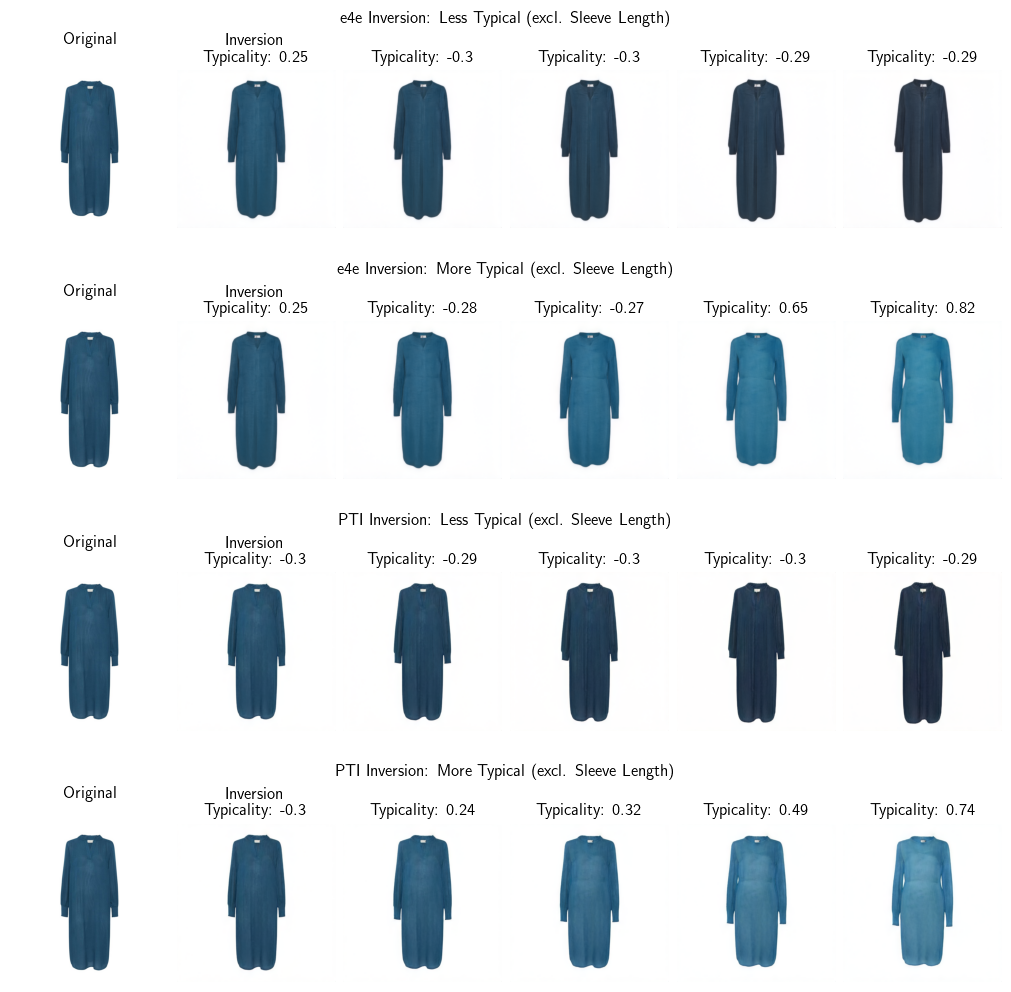
\includegraphics[width=1\linewidth]{Thesis/Results/assets/disentangled_excl_sleeve_main_result.png}
    \caption[Typicality Manipulations using Disentangled Embeddings excl. sleeve length]{Typicality Manipulations using Disentangled Embeddings excl. Sleeve Length}
    \label{fig:disentangled_excl_sleeve_main_result}
\end{figure}
\textbf{Conditional manipulation} using physical attributes like sleeve length can offer valuable insights into the manipulation behavior. By excluding the sleeve length sub-embedding from the disentangled embeddings, the typicality calculation ignores this attribute. During manipulation, this conditioning ensures that the sleeve length cannot change when altering typicality. The results of this conditional typicality manipulation are shown in \ref{fig:disentangled_excl_sleeve_main_result} and \ref{fig:disentangled_ex_sleeve_more}. Since here the typicality manipulation does not entail changes in the sleeve lengths, conditioning works successfully. Additionally, without access to the sleeve length attribute, the manipulations become subtler, focusing instead on adjusting the fit around the waist and making slight color changes. These modifications are consistent with the most and least typical images based on disentangled embeddings excluding sleeve length, as seen in figure \ref{fig:examples_disentangled_ex_sleevel_length}. When applying the same conditioning approach using color as the attribute, the model again relies on sleeve length, as in the unconditional case (see figure \ref{fig:disentangled_ex_color_more}). These experiments reveal that the manipulation model based on disentangled embeddings always opts for the quickest path to typicality, which typically involves altering sleeve lengths. If this attribute is restricted, the model shifts to the next most effective path, adjusting shape and color. This demonstrates that typicality in disentangled embeddings is multi-dimensional, with each dimension contributing to the manipulation of a dress's typicality. Without conditioning, the model naturally selects the most dominant attribute for manipulation. To determine whether this behavior is unique to disentangled typicality manipulation, conditional manipulation was also tested with DINOv2-based typicality scores. Since the unconditional manipulations in this case primarily relied on shape and color, conditioning on color was examined. Conditioning on shape was not feasible due to a mismatch between the dataset's shape attribute and the actual changes seen in manipulation. Results of the color-conditioned typicality manipulation of DINOv2-based embeddings can be found in figure \ref{fig:dino_cond_color_more}. Here it becomes clear, that the conditioning approach in InterFaceGAN does not effectively constrain the color attribute, as the model continues to alter the color of dresses. Furthermore, no significant difference is observed compared to the unconditional manipulation. This indicates that DINOv2-based typicality is driven by a single dimension of typicality, in contrast to the richer, multi-dimensional nature of disentangled embeddings. It is also important to note that the two conditioning methods are not directly methodologically comparable, with one being a post-processing approach, while the other is a complete re-calculation of the typicality measures conditioned on an attribute. For the simple DINOv2 embeddings, conditioning entails ex-post transformation through a projection of the typicality boundary with the respective boundary of the physical attribute, as described in section \ref{sec:interfacegan}. For the typicality measure based on disentangled embeddings, conditional manipulation works by calculating a separate typicality measure and InterFaceGAN boundary based on a concatenation of all sub-embeddings excluding the respective sub-embedding for the attribute at hand.


\textbf{Differences between e4e and PTI inversions} with respect to the manipulation performance can be observed in all result figures. Specifically, generations using PTI inversions tend to deteriorate in quality as the manipulation distance increases. Although PTI reconstructions are generally better than e4e inversions, the last few manipulation steps, i.e. 15-20 unit-normal vector steps away from the reconstruction, often show a decline in image quality. This is likely because the fine-tuned generator in PTI is optimized for the area around the initial reconstruction. When manipulations are performed in the latent space, the resulting latent codes might fall outside the region for which the fine-tuned generator was optimized. This phenomenon is not equally present in all examples. Easy-to-invert dresses require fewer changes in the generator weights, thus being closer to the original generator that can operate well on the whole latent space. For those dresses, quality deterioration is not an issue. However, for dresses with complex patterns or shapes, image quality tends to decline as the distance from the initial reconstruction increases. This observation holds true for both typicality measures.

\FloatBarrier



\section{Discussion}
The goal of this work was the development of a fine-grained typicality manipulation method and the
exploration of various techniques to solve the various sub-tasks needed for this. While this goal and the desired main contribution have been achieved, a more detailed look at the implications of the results is necessary before concluding this work. Using two typicality measurements and two inversion techniques in the final experiments, the advantages and disadvantages of each combination of methods can be deducted when looking at the results presented in section \ref{sec:results}. Comparing the manipulation performance between DINOv2-based typicality scores and those based on disentangled embeddings reveals a clear trade-off between disentanglement and interpolability. Disentangled embeddings offer a rich, multi-dimensional understanding of typicality, while DINOv2-based embeddings are simpler, allowing only one-dimensional typicality manipulations. Attempts to disentangle manipulations from DINOv2-based typicality scores through conditioning were unsuccessful, which can be seen as a limitation of this work, although the overall typicality manipulations still produced satisfactory results. The advantage of the richer disentangled embeddings lies in the possibility of conditional, attribute-specific typicality manipulation, as shown with the sleeve length attribute conditioning. On the other hand, typicality manipulation based on disentangled embeddings does not always allow smooth and thus controlled interpolation. When traversing the latent space, sudden jumps in typicality scores and drastic changes in physical attributes can occur for some samples. To address this problem, a smoother distribution of typicality scores, on which latent space editing directions are based, is needed. This could be achieved by significantly expanding the dataset size. However, this was not possible during this work due to the limited number of articles available on "zalando.de". To artificially increase the dataset size, one could add data augmentations by manipulating images using the techniques described in this work and learning typicality scores based on the augmented dataset. This approach could be explored in future research to further improve typicality manipulation. For practitioners, this trade-off between disentanglement and interpolability is difficult to solve and the selection of the suitable approach often depends on the specific use-case. In high fashion, where a designer's creation is valued highly, often subtle changes in the design are desired. Here, using a simple typicality measure might be sufficient, since the changes applied can be much more subtle and the typicality scores change smoothly. However, for fast prototyping and automated design optimization, disentangled embeddings, that allow more control over the different attributes and that result in more drastic changes in the design are suitable.\\
Comparing the manipulation performance of the two tested inversion methods, a trade-off between reconstruction quality and editing performance becomes clear. While PTI is capable of reconstructing especially complicated samples much more realistically, its editing performance can degrade with the manipulation strength. The basic e4e inversion on the other hand lacks reconstruction quality but is capable of producing latent codes that are easily editable even into far regions of the latent space. Furthermore, PTI is significantly slower in producing inversions. Again, the selection of the correct approach depends on the specific use case and requirements a designer has for the design augmentation tool. For applications that require fast inference and strong manipulations, i.e. large steps in the latent space, e4e is the logical choice. However, if samples are difficult to invert or if the manipulation needs to be subtle, i.e. taking small steps in the latent space, using PTI is preferred. \\
Although the generated images from the GAN model and the inversion techniques are generally of high quality, artifacts can still occur in some generations. This is especially the case when the manipulation reaches ill-defined regions of the latent space. However, artifacts can also arise in any generation produced by the custom StyleGAN2-Ada model or any inversion technique. These quality issues highlight a weakness of using GANs compared to diffusion models, which typically produce images of higher quality. The main reason for using GAN-based techniques in this work was the well-behaved latent space of GANs.  However, with the growing popularity of diffusion models for image generation, new methods for image manipulation using these models are being published more frequently. During the duration of this thesis, several promising approaches for attribute manipulation with diffusion models were published. New techniques claim to have found methods to create a disentangled latent space for diffusion models similar to the StyleGAN latent space (e.g. \cite{dravid2024interpreting}). Exploring these techniques for typicality manipulation could be a promising direction for future research.
\section{Conclusion}
This thesis investigated the manipulation of design typicality in fashion with generative deep neural networks, with a particular focus on the category of women's dresses. By leveraging the capabilities of the StyleGAN2-Ada model, the study aimed to adjust the typicality of fashion designs, a key aesthetic attribute linked to consumer preferences, while maintaining the overall integrity and coherence of the generated images. In this work, various techniques have been explored to achieve the sub-tasks of image generation, GAN inversion, typicality measurement, and latent space editing. The findings demonstrate that typicality can be effectively manipulated within the latent space of the StyleGAN2-Ada model, utilizing inversion techniques such as e4e and PTI. A supervised latent space manipulation method, InterFaceGAN, was successfully applied to achieve typicality editing. These results suggest that this approach could be a valuable tool for designers, enabling them to refine product designs in line with consumer expectations.
However, the study also highlighted several limitations and trade-offs. Notably, a trade-off between disentanglement and interpolability was observed in the two typicality measurements used. Additionally, a trade-off between inversion quality and editing performance was identified when comparing e4e and PTI inversions. In summary, this work contributes to the understanding of how generative models can be used to manipulate aesthetic attributes in fashion design. While further research is needed, the findings offer a foundation for future exploration in this area and potential applications in the design process.

%%%%%%%%%%%%%%%%%%% References 
\addcontentsline{toc}{section}{References}    
\bibliographystyle{apalike}
\clearpage
\pagenumbering{roman}
\bibliography{bib_file}                     
\newpage

%%%%%%%%%%%%%%%%%%%% Appendix
\clearpage % Ensure it starts on a new page
\phantomsection
\addcontentsline{toc}{section}{Appendix}  
\appendix
\pagenumbering{roman}% resets `page` counter to 1
\section*{Appendix}

% New Figure Counter for Appendix with A. prefix
\counterwithin*{figure}{part}
\stepcounter{part}
\renewcommand{\thefigure}{A.\arabic{figure}}

\FloatBarrier
\subsection*{GAN Inversion}
\begin{figure}[!ht]
    \centering
    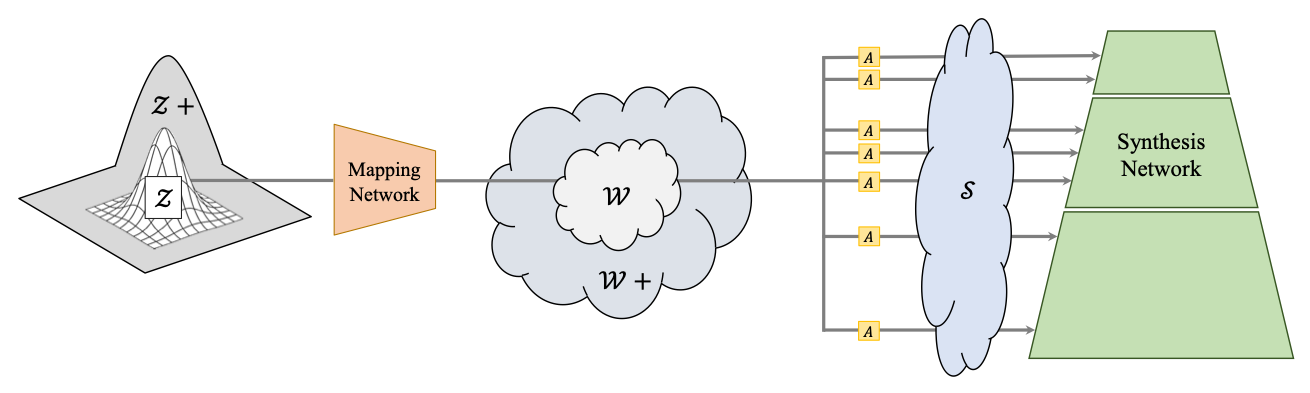
\includegraphics[width=1\linewidth]{Thesis/Background/assets/latent_spaces.png}
    \caption[StyleGAN Latent Spaces]{StyleGAN Latent Spaces - taken from \cite{bermano2022state}}
    \label{fig:latent_spaces}
\end{figure}

\begin{figure}[!ht]
    \centering
    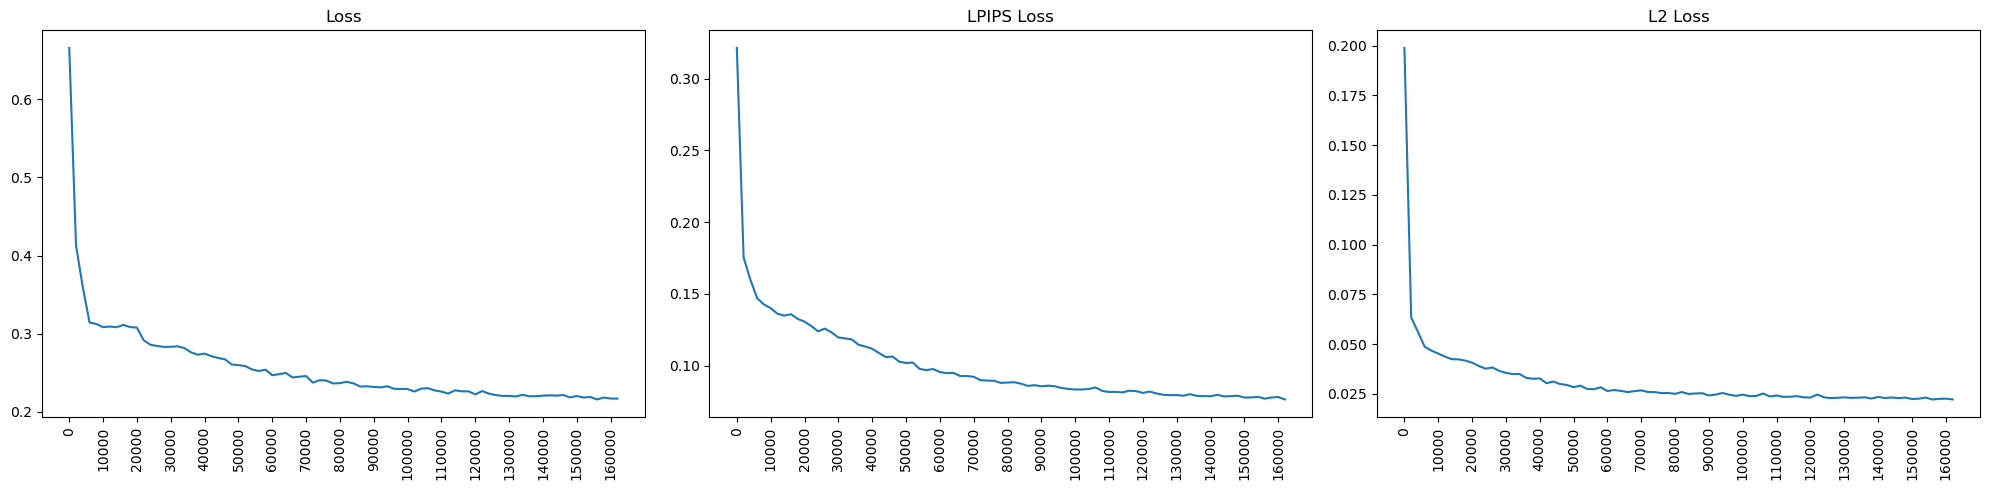
\includegraphics[width=1\linewidth]{Thesis/Method/assets/e4e_loss_curves.png}
    \caption{encoder4editing Training Loss Curves}
    \label{fig:e4e_loss_curves}
\end{figure}

\begin{figure}[!ht]
     \centering
     \begin{subfigure}[b]{1\textwidth}
         \centering
         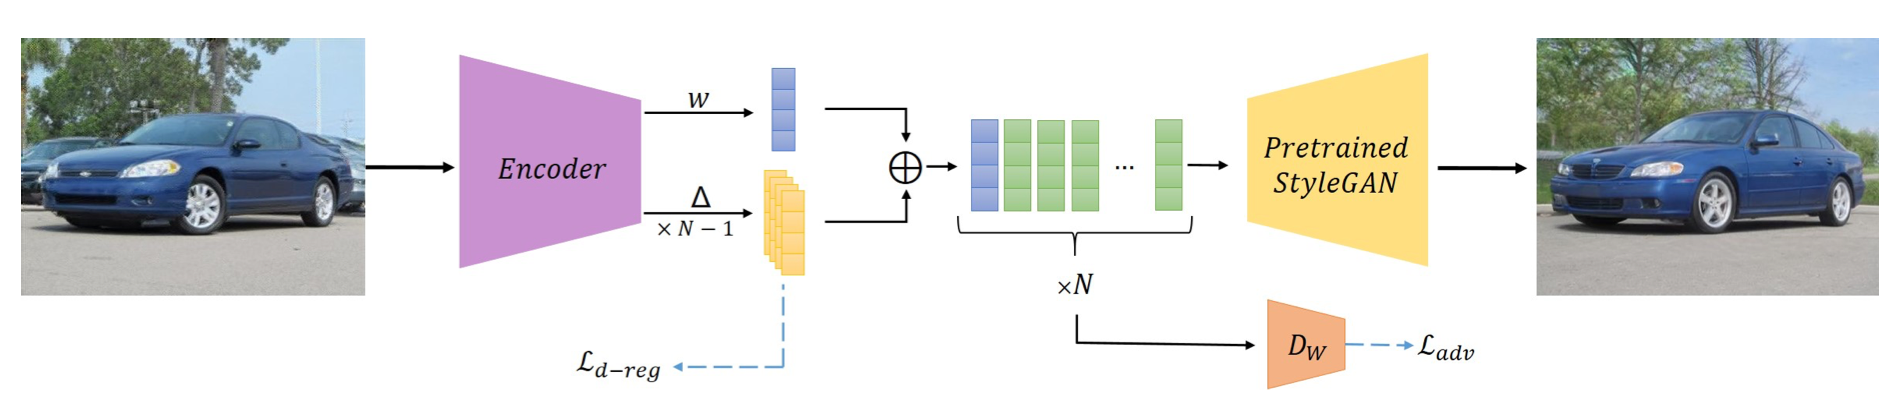
\includegraphics[width=0.95\linewidth]{Thesis/Background/assets/e4e.png}
         \caption{encoder4editing - taken from \cite{tov2021designing}}
         \label{fig:e4e}
     \end{subfigure}
     \hfill
     \begin{subfigure}[b]{1\textwidth}
         \centering
         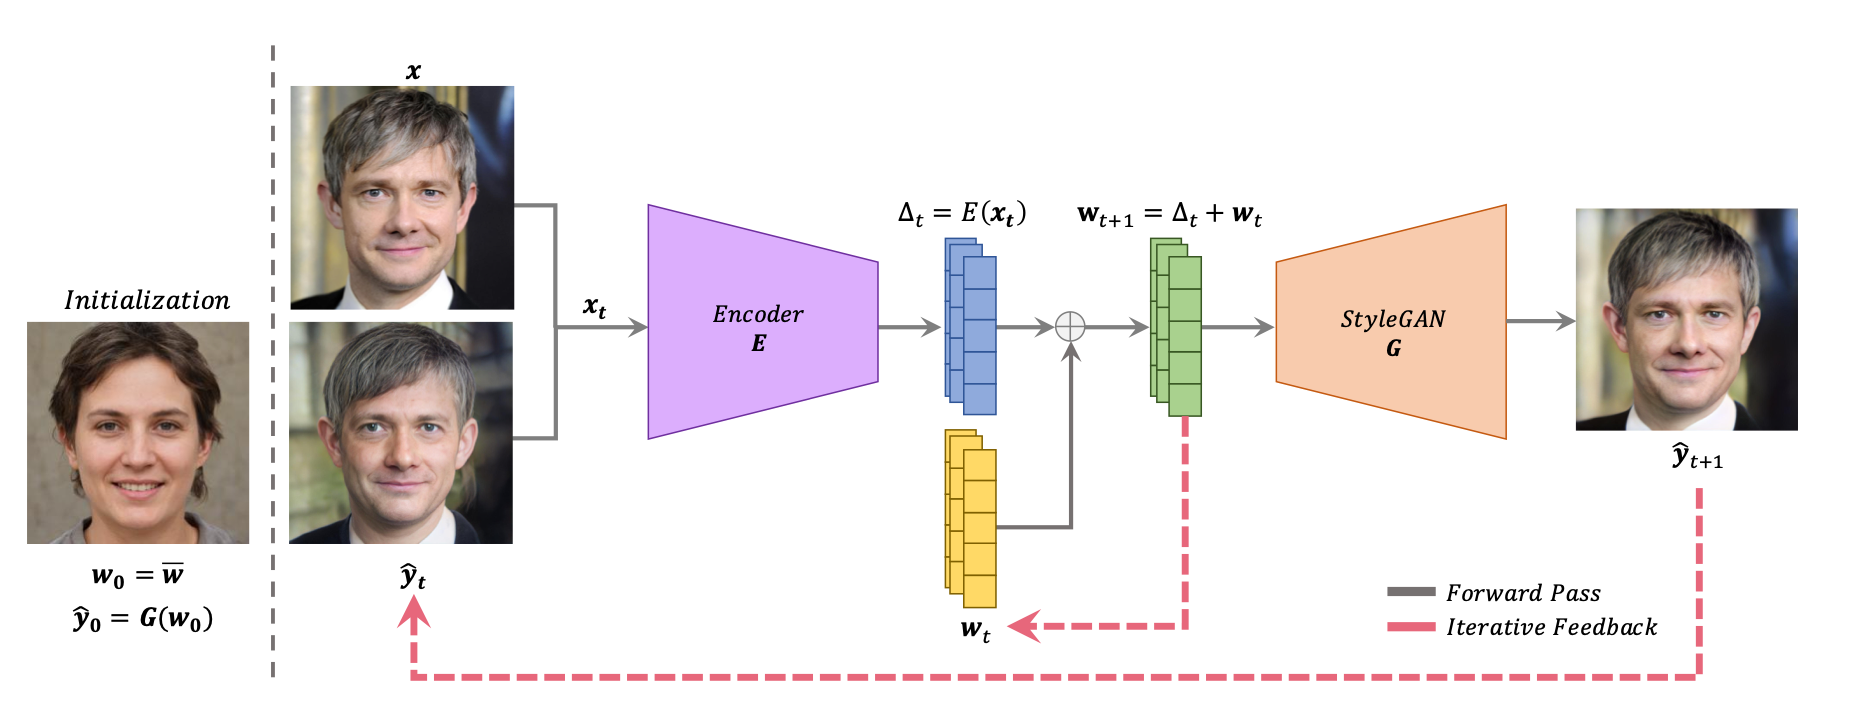
\includegraphics[width=0.95\linewidth]{Thesis/Background/assets/restyle.png}
         \caption{ReStyle - taken from \cite{alaluf2021restyle}}
         \label{fig:restyle}
     \end{subfigure}
     \hfill
     \begin{subfigure}[b]{1\textwidth}
         \centering
         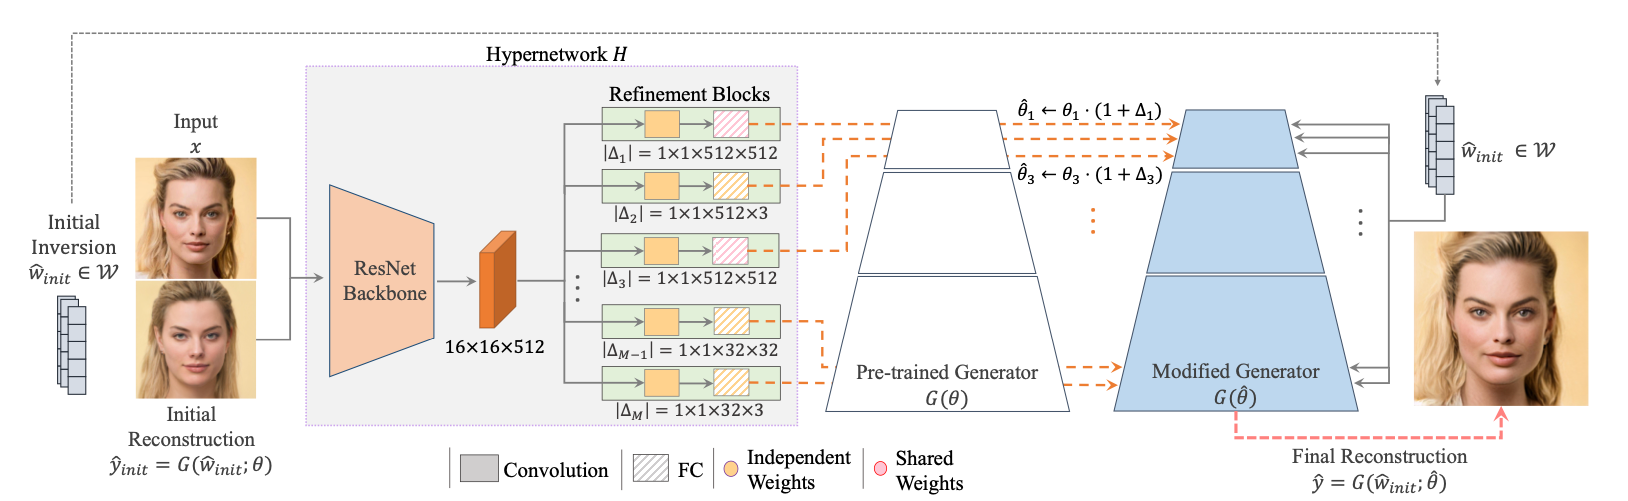
\includegraphics[width=0.95\linewidth]{Thesis/Background/assets/hyperstyle.png}
         \caption{HyperStyle - taken from \cite{alaluf2022hyperstyle}}
         \label{fig:hyperstyle}
     \end{subfigure}
        \caption{Schematic Overview of Inversion Methods}
        \label{fig:inversion_methods}
\end{figure}

\FloatBarrier
\clearpage
\subsection*{StyleGAN2-Ada Training}
\begin{figure}[ht!]
    \centering
    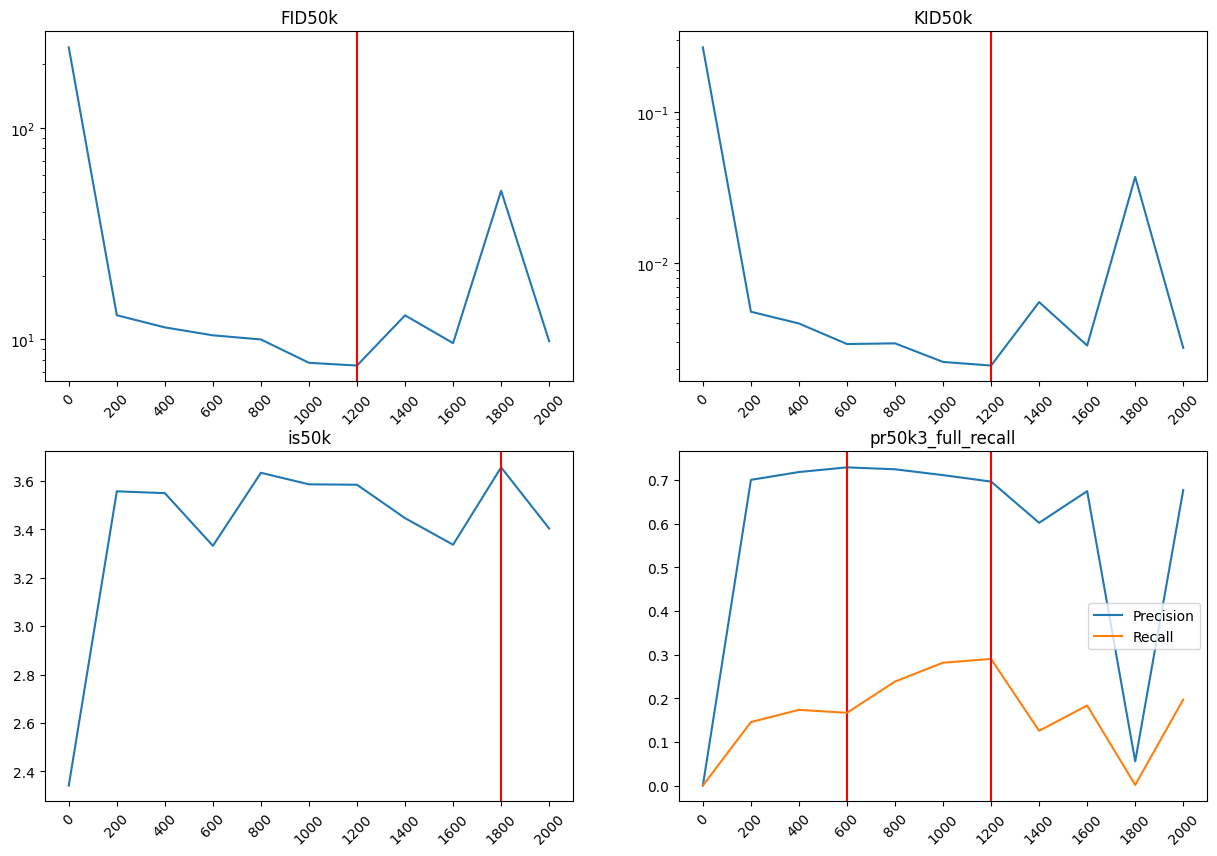
\includegraphics[width=1\linewidth]{Thesis/Results/assets/sg2ada_evaluation_metrics.png}
    \caption[StyleGAN2-Ada Training Evaluation]{StyleGAN2-Ada Training Evaluation: \textit{Red lines indicate best values within each metric. FID50k, KID50k, and IS50k refer to the FID, KID, and IS calculated based on 50k generated images.}}
    \label{fig:sg2ada_evaluation_metrics}
\end{figure}

\FloatBarrier
\clearpage
\subsection*{InterFaceGAN}
\begin{figure}[!ht]
    \centering
    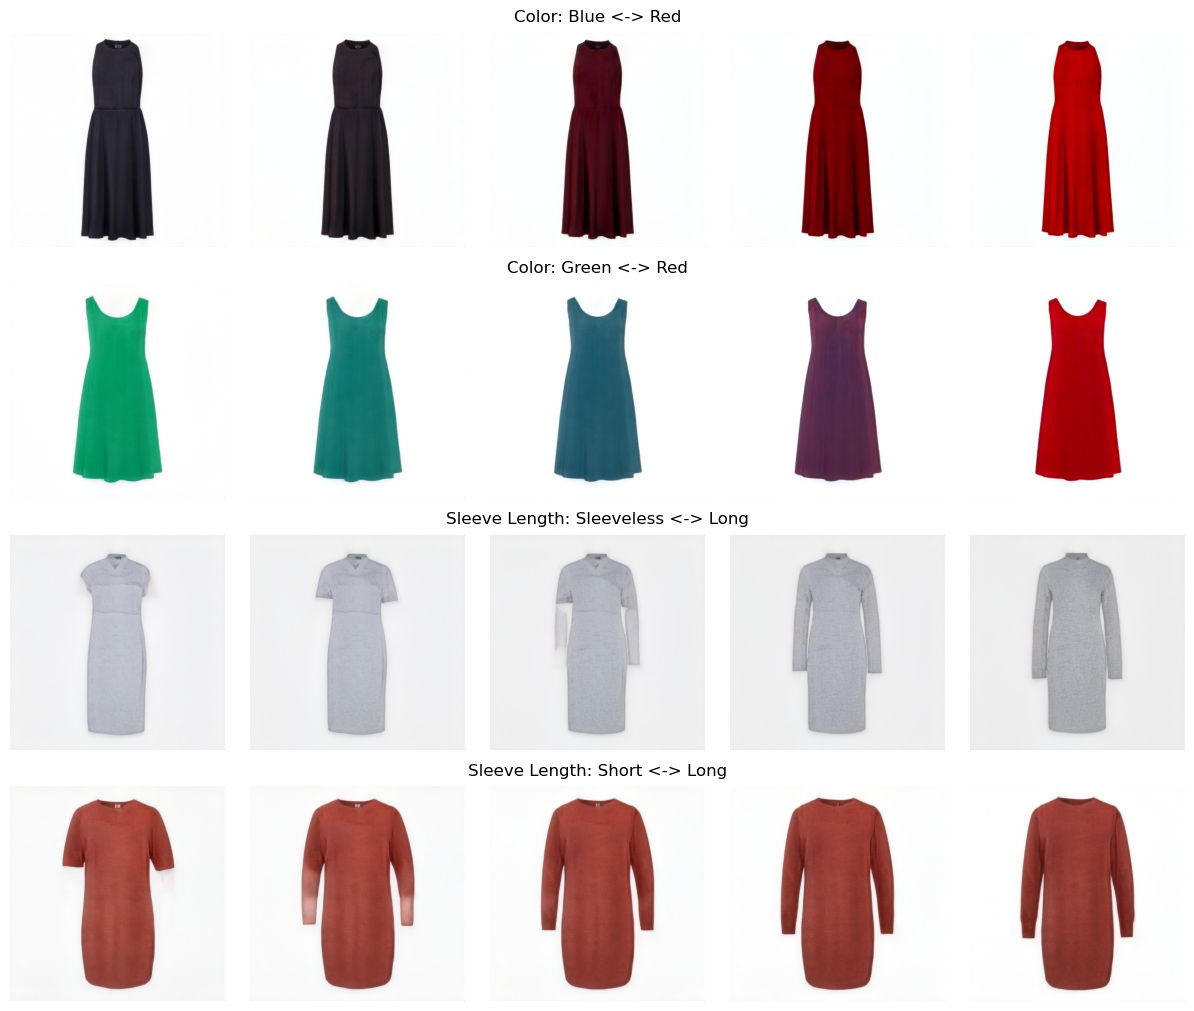
\includegraphics[width=1\linewidth]{Thesis/Method/assets/physical_attributes_manipulation.png}
    \caption[Manipulations of Physical Attributes Used as Conditions]{Manipulations of physical attributes used as conditions: \textit{Physical attributes are used as conditional boundaries for the typicality manipulation. To visually validate that the boundaries are meaningful, one can look at manipulations using the boundaries. All images are generated from e4e inversions.}}
    \label{fig:physical_attributes_manipulation}
\end{figure}


\begin{table}[ht]
\centering
\begin{tabular}{|c|c|c|}
\hline
       &      Color &   Sleeve Length \\
\hline
 count & 91      &         54      \\
 mean  &  0.9595 &          0.9673 \\
 std   &  0.0324 &          0.0506 \\
 min   &  0.8736 &          0.7647 \\
 25\%   &  0.9359 &          0.965  \\
 50\%   &  0.9694 &          0.9885 \\
 75\%   &  0.9859 &          0.9962 \\
 max   &  1      &          1      \\
\hline
\end{tabular}
\caption{Summary Statistics of Separation Performance for Physical Attributes}
\label{tab:physical_summary_stats}
\end{table}

\FloatBarrier
\subsection*{Typicality Measurements}
\begin{figure}[!ht]
    \centering
    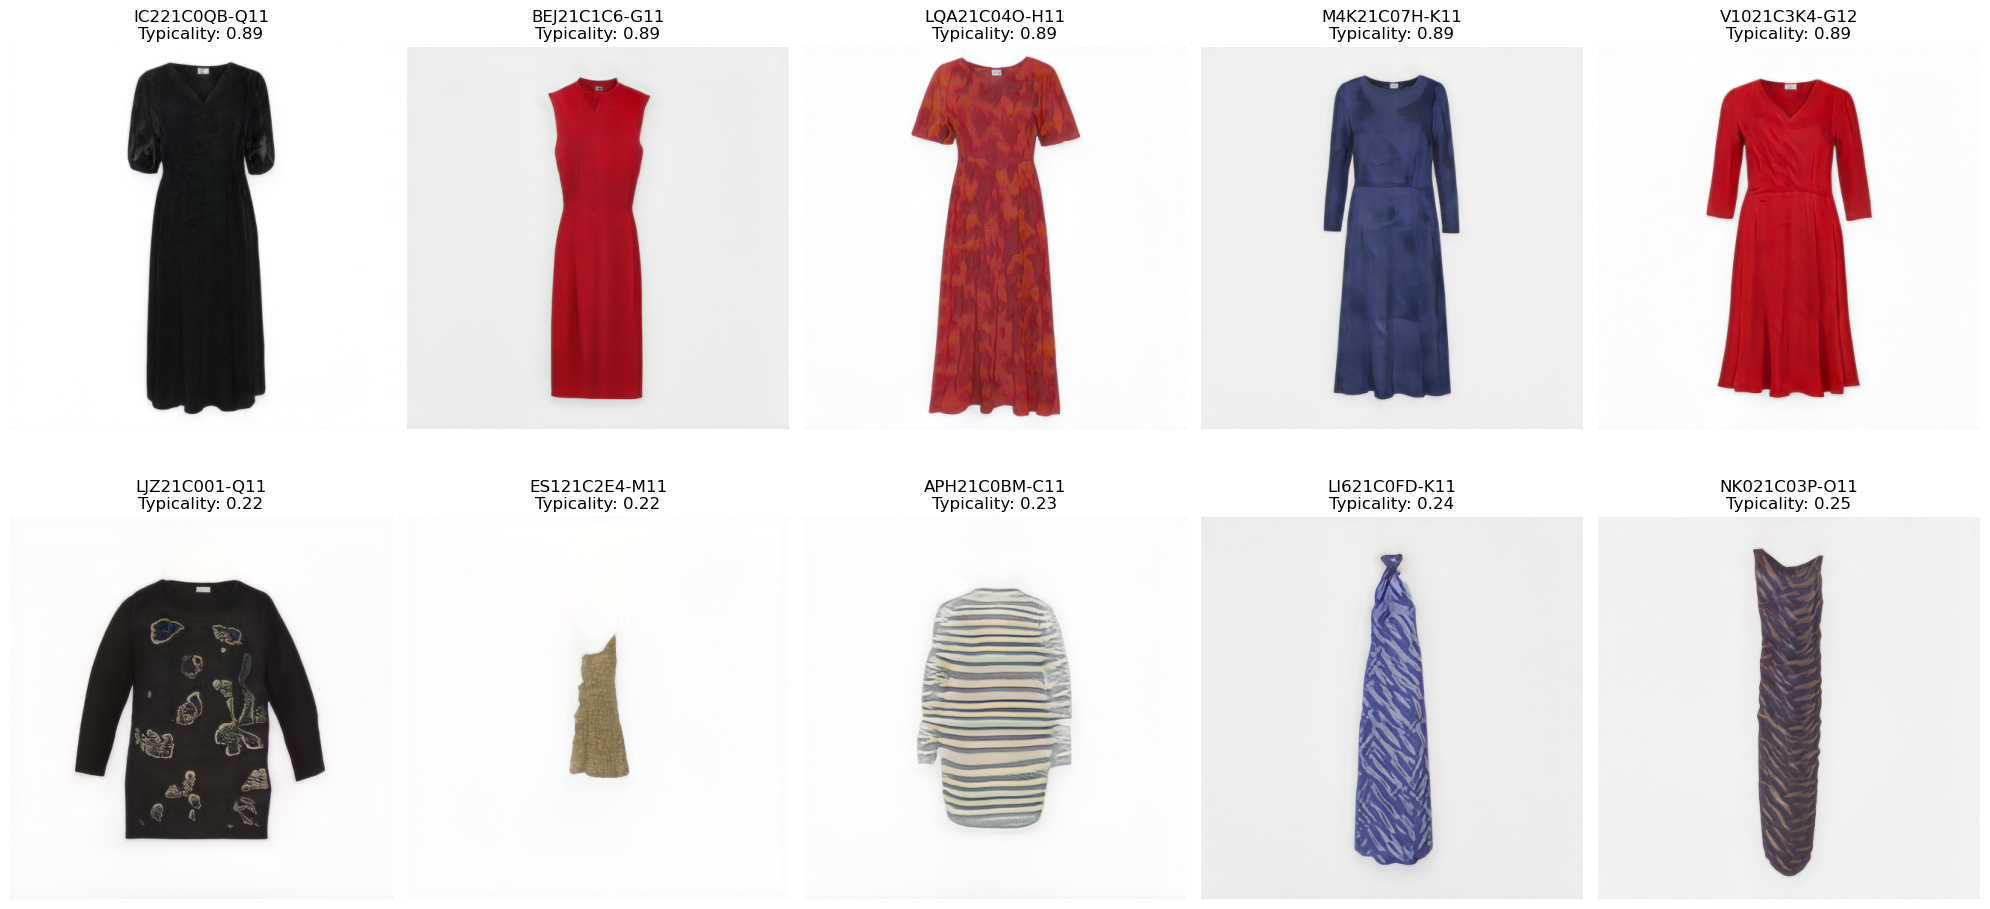
\includegraphics[width=1\linewidth]{Thesis/Results/assets/examples_dino_typicality.png}
    \caption[Most and Least Typical Dresses based on DINOv2 Embeddings]{Most and Least Typical Dresses based on DINOv2 Embeddings: \textit{Top row shows samples with the highest typicality scores, bottom row shows samples with the lowest typicality scores}}
    \label{fig:examples_dino_typicality}
\end{figure}

\begin{figure}[!ht]
    \centering
    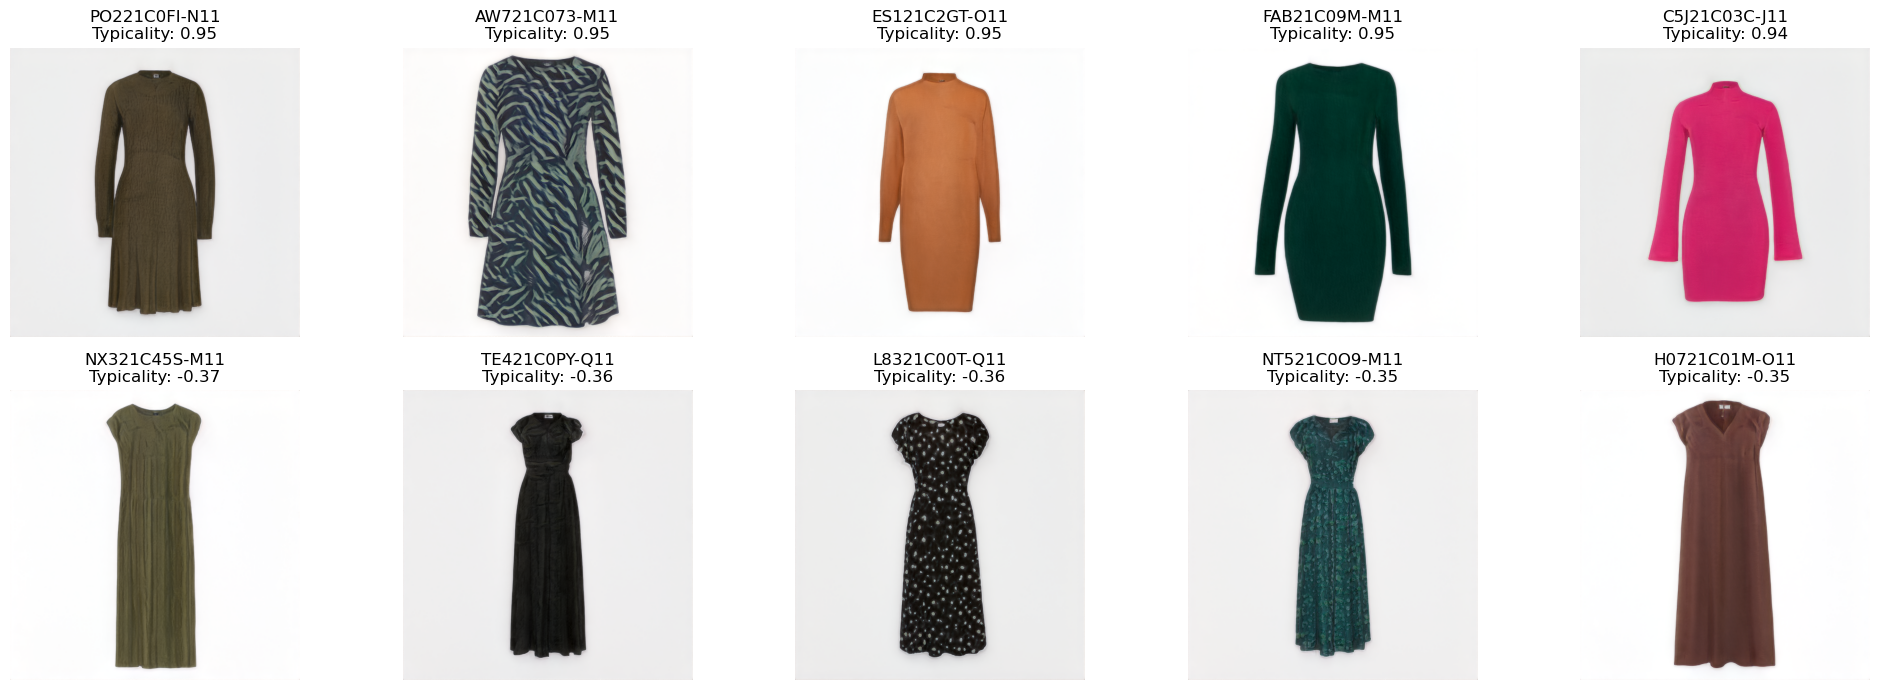
\includegraphics[width=1\linewidth]{Thesis/Results/assets/examples_disentangled_typicality.png}
    \caption[Most and Least Typical Dresses based on Complete Disentangled Embeddings]{Most and Least Typical Dresses based on Complete Disentangled Embeddings: \textit{Top row shows samples with the highest typicality scores, bottom row shows samples with the lowest typicality scores}}
    \label{fig:examples_disentangled_typicality}
\end{figure}

\begin{figure}[!ht]
    \centering
    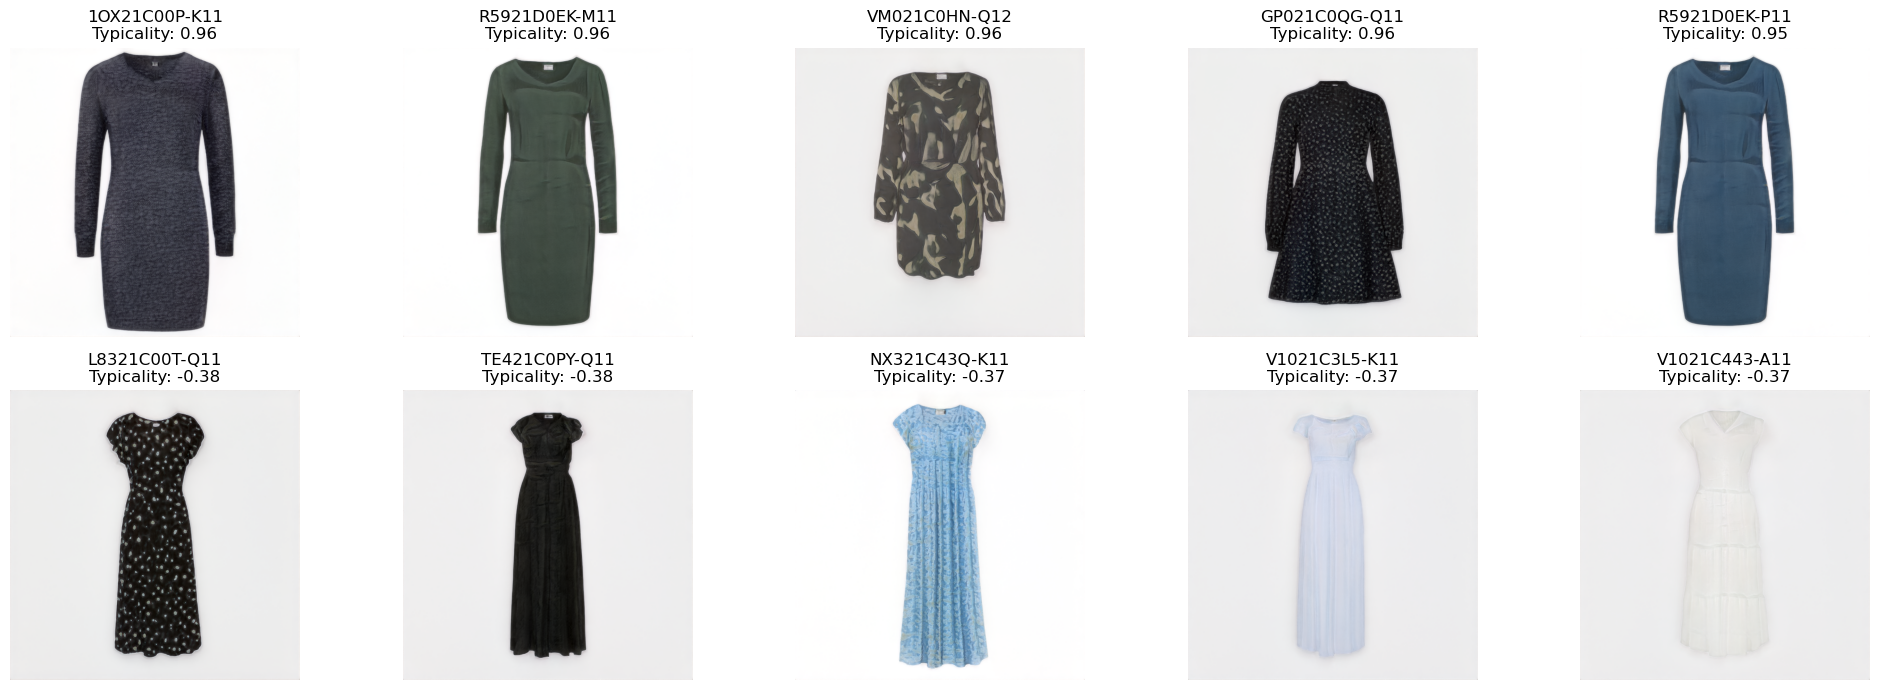
\includegraphics[width=1\linewidth]{Thesis/Results/assets/examples_disentangled_ex_color.png}
    \caption[Most and Least Typical Dresses based on Disentangled Embeddings excluding Color]{Most and Least Typical Dresses based on Disentangled Embeddings excluding Color: \textit{Top row shows samples with the highest typicality scores, bottom row shows samples with the lowest typicality scores}}
    \label{fig:examples_disentangled_ex_color}
\end{figure}

\begin{figure}[!ht]
    \centering
    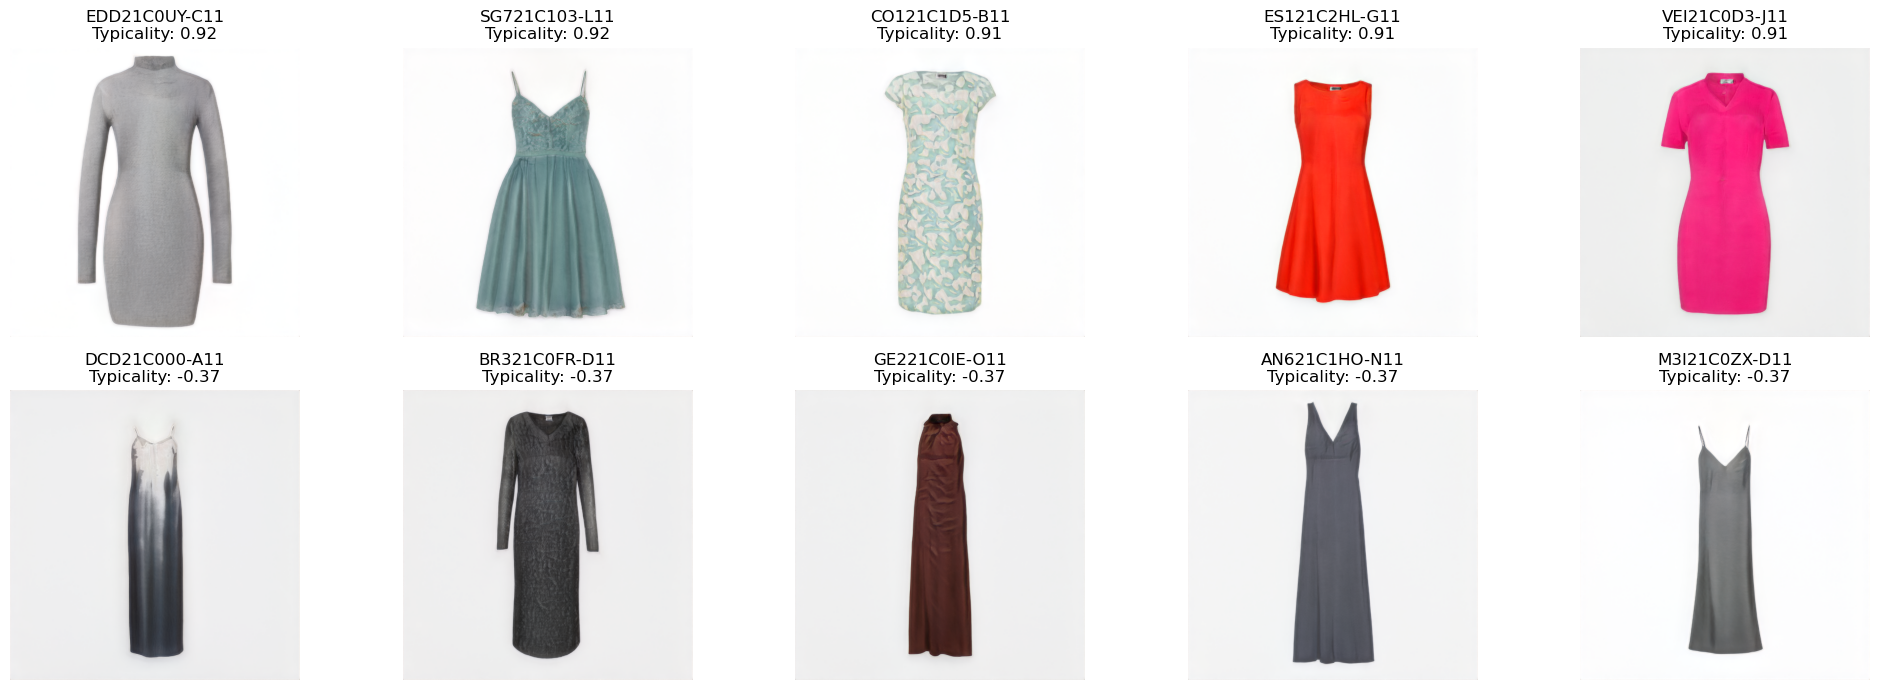
\includegraphics[width=1\linewidth]{Thesis/Results/assets/examples_disentangled_ex_sleevel_length.png}
    \caption[Most and Least Typical Dresses based on Disentangled Embeddings excluding Sleeve Length]{Most and Least Typical Dresses based on Disentangled Embeddings excluding Sleeve Length: \textit{Top row shows samples with the highest typicality scores, bottom row shows samples with the lowest typicality scores}}
    \label{fig:examples_disentangled_ex_sleevel_length}
\end{figure}

\begin{figure}[!ht]
     \centering
     \begin{subfigure}[b]{0.48\textwidth}
         \centering
         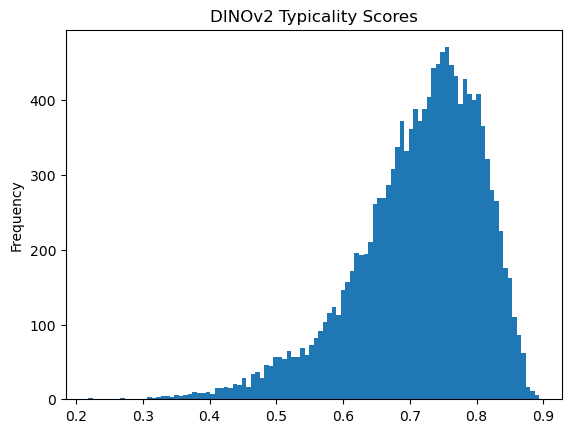
\includegraphics[width=\textwidth]{Thesis/Results/assets/distribution_dino_typicality.png}
         \caption{DINOv2 Embeddings}
     \end{subfigure}
     \hfill
     \begin{subfigure}[b]{0.48\textwidth}
         \centering
         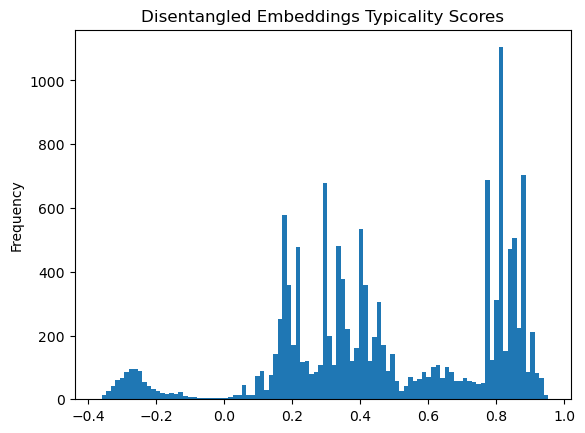
\includegraphics[width=\textwidth]{Thesis/Results/assets/distribution_disentangled_typicality.png}
         \caption{Disentangled Embeddings}
     \end{subfigure}
     \hfill
\caption{Distribution of typicality scores}
\label{fig:typicality_score_distribution}
\end{figure}

\FloatBarrier
\subsection*{Hyperstyle Manipulation Results}
\begin{figure}[!ht]
    \centering
    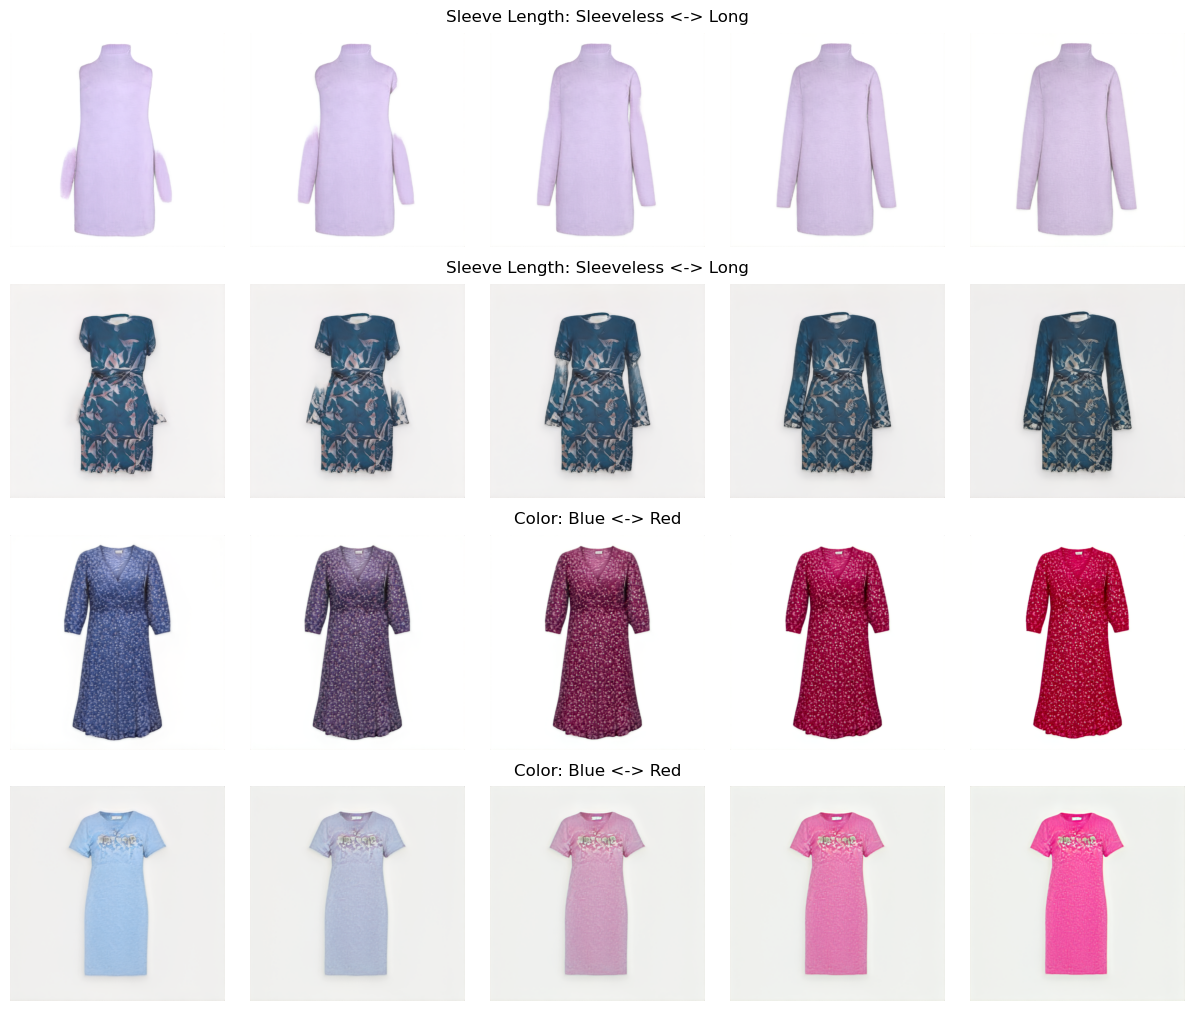
\includegraphics[width=1\linewidth]{Thesis/Results/assets/hyperstyle_manipulation_tests.png}
    \caption[Preliminary Manipulation Tests using Hyperstyle Inversions]{Preliminary Manipulation Tests using Hyperstyle Inversions: \textit{To assess the overall suitability of Hyperstyle Inversions for the InterFaceGAN scheme, manipulation of visual attributes is tested. Although some manipulations seem to work well, others, especially the sleeve length manipulations, produce faulty artifacts.}}
    \label{fig:hyperstyle_manipulation_tests}
\end{figure}


\FloatBarrier
\newpage
\subsection*{Distance Correlation Formulas}
Below, detailed formulas for the calculation of the distance correlation are given. All formulas and explanations are directly taken or slightly adapted from \cite{muller2024disentangling}, p.5.
\begin{equation}\label{eq:dcor_formula}
\text{dCor}(w_1, w_2) = \sqrt{\frac{\text{dCov}^2(w_1, w_2)}{(\text{dVar}^2(w_1) \text{dVar}^2(w_2))^{1/2}}}
\end{equation}

Assuming \(n\)-dimensional batches of subspace vectors \(w_1 \in \mathbb{R}^{n \times d_1}\) and \(w_2 \in \mathbb{R}^{n \times d_2}\), a \(n \times n\) dimensional Euclidean space containing all pairwise distances can be calculated as
\begin{equation}
A \in \mathbb{R}^{n \times n}, \quad a_{j,k} = \|w_1^{(j)} - w_1^{(k)}\|_2, \quad j, k = 1, 2, \dots, n
\end{equation}
\begin{equation}
B \in \mathbb{R}^{n \times n}, \quad b_{j,k} = \|w_2^{(j)} - w_2^{(k)}\|_2, \quad j, k = 1, 2, \dots, n
\end{equation}

Normalization of the distance matrices was performed by subtracting the row mean, column mean, and grand mean. Formally, this can be expressed as
\begin{equation}
A_{j,k} := a_{j,k} - \bar{a}_{j,\cdot} - \bar{a}_{\cdot,k} + \bar{a}_{\cdot,\cdot}
\end{equation}
\begin{equation}
B_{j,k} := b_{j,k} - \bar{b}_{j,\cdot} - \bar{b}_{\cdot,k} + \bar{b}_{\cdot,\cdot}
\end{equation}

Finally, $\text{dCov}^2$ can be calculated as the arithmetic mean of the element-wise matrix product.
\begin{equation}
\text{dCov}^2(w_1, w_2) = \frac{1}{n^2} \sum_{j=1}^{n} \sum_{k=1}^{n} A_{j,k} B_{j,k}
\end{equation}
$\text{dVar}^2$ can be calculated as the arithmetic mean of the squared matrix elements of the normalized distance matrices.
\begin{equation}
\text{dVar}^2(w_1) = \frac{1}{n^2} \sum_{j,k} A_{j,k}^2
\end{equation}
\begin{equation}\label{eq:last_dcor_formula}
\text{dVar}^2(w_2) = \frac{1}{n^2} \sum_{j,k} B_{j,k}^2
\end{equation}

\FloatBarrier

%\subsection*{Unconditional Typicality Manipulation}

\clearpage
\begin{figure}[!ht]
    \centering
    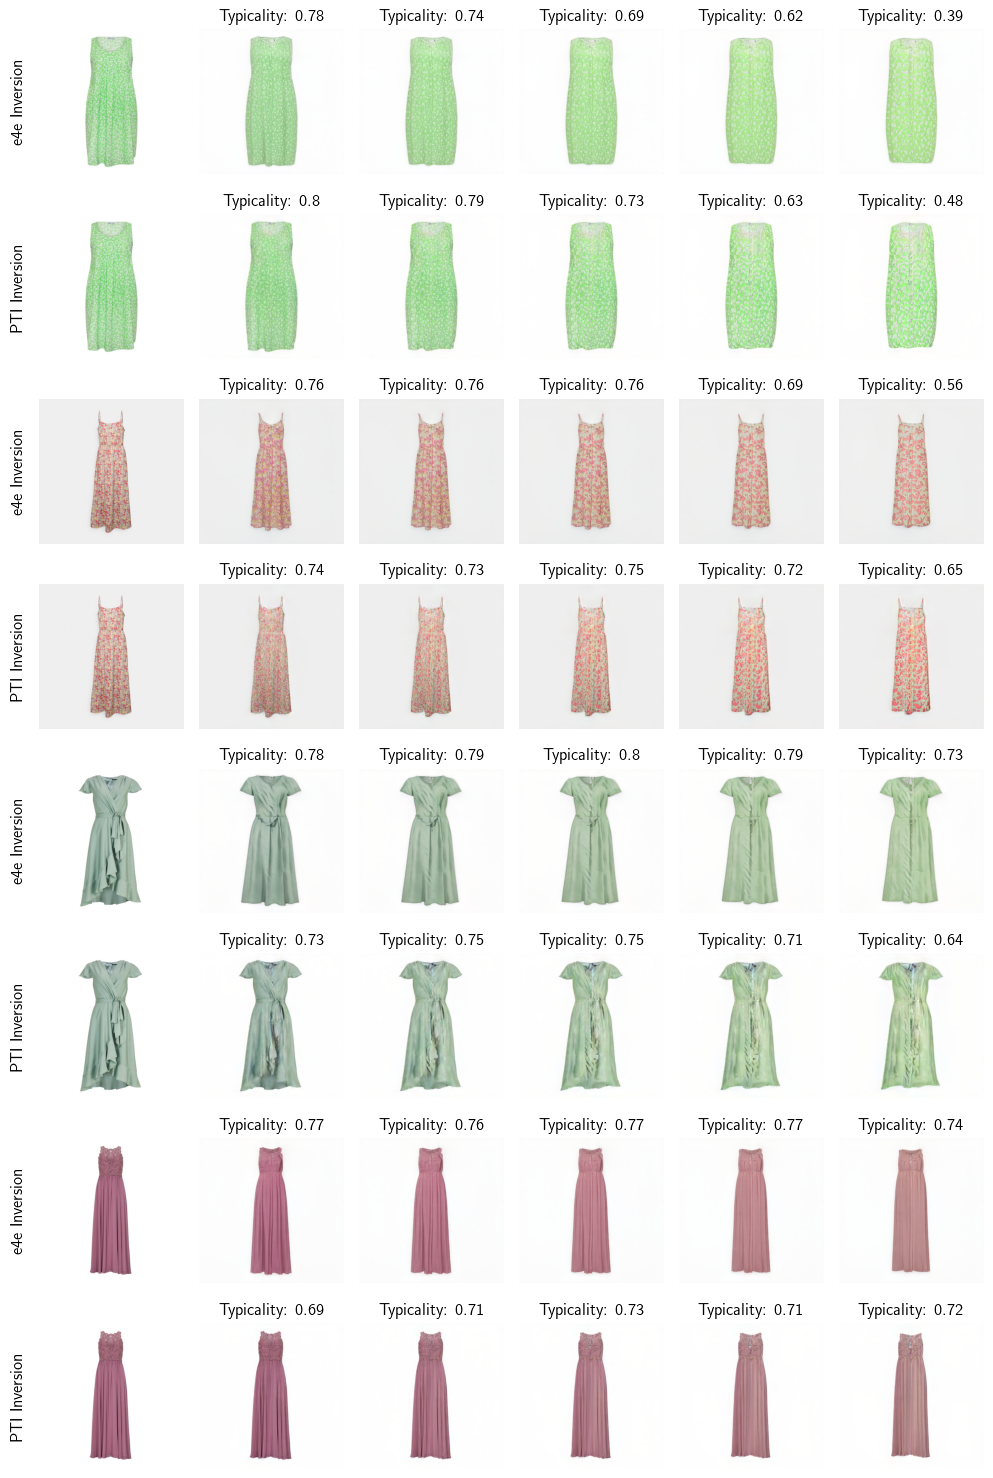
\includegraphics[width=0.9\linewidth]{Thesis/Results/assets/dino_less.png}
    \caption[Decreasing Typicality for DINOv2 Embeddings]{Decreasing Typicality for DINOv2 Embeddings: \textit{First row shows the original image, second row is the inversion. All following rows are each +5 InterFaceGAN steps towards less typicality}}
    \label{fig:dino_less}
\end{figure}

\clearpage
\begin{figure}[!ht]
    \centering
    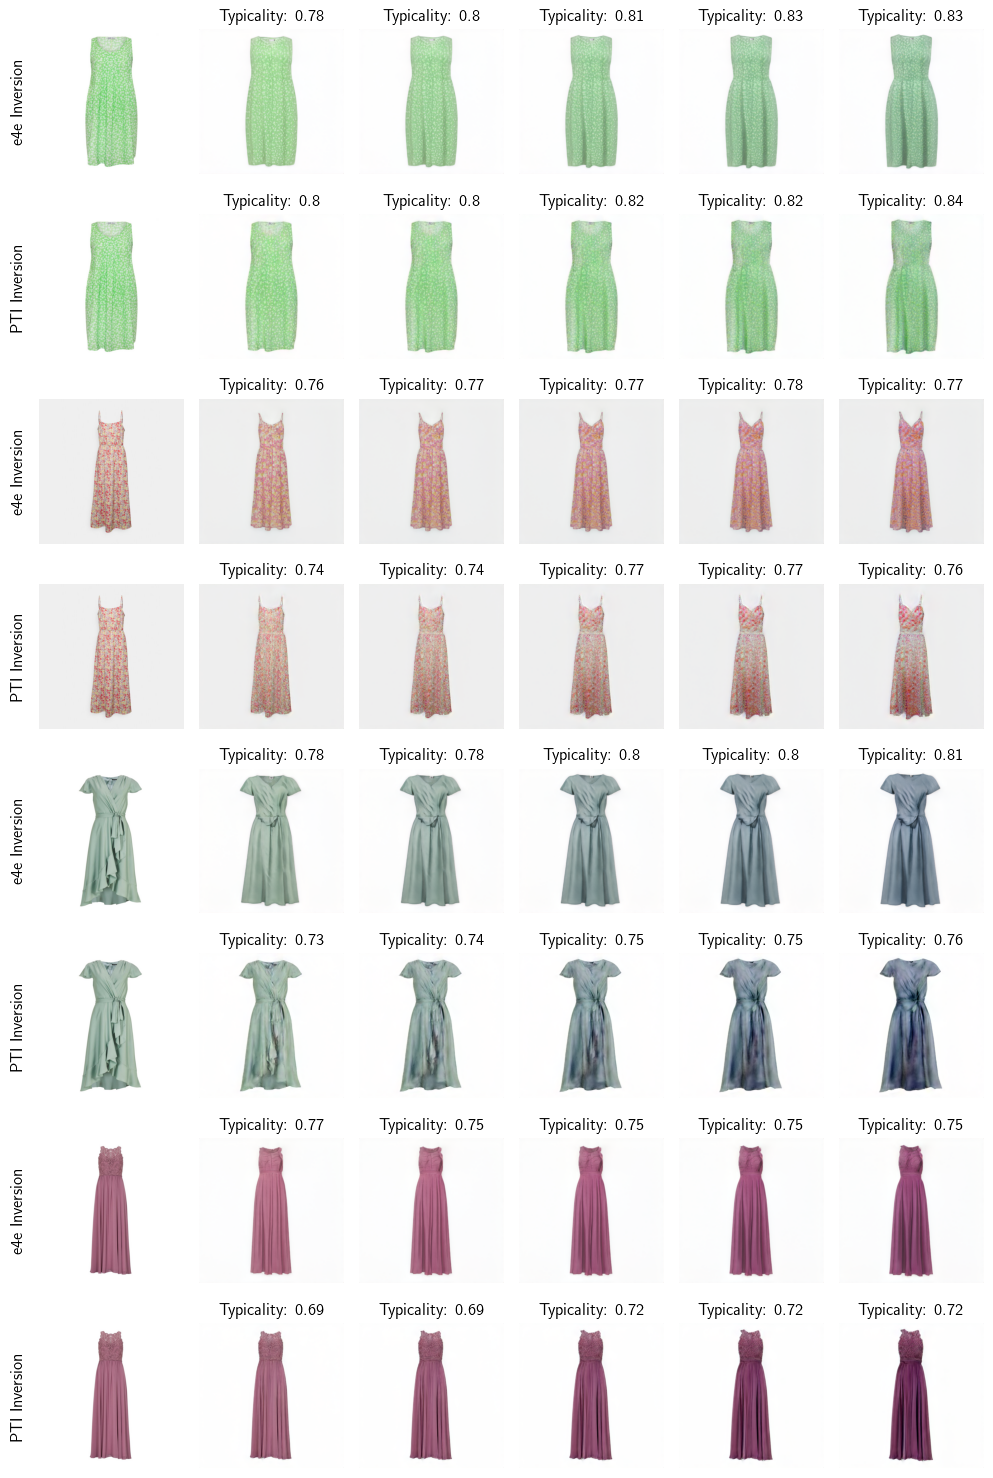
\includegraphics[width=0.9\linewidth]{Thesis/Results/assets/dino_more.png}
    \caption[Increasing Typicality for DINOv2 Embeddings]{Increasing Typicality for DINOv2 Embeddings: \textit{First row shows the original image, second row is the inversion. All following rows are each +5 InterFaceGAN steps towards more typicality}}
    \label{fig:dino_more}
\end{figure}


\clearpage
\begin{figure}[!ht]
    \centering
    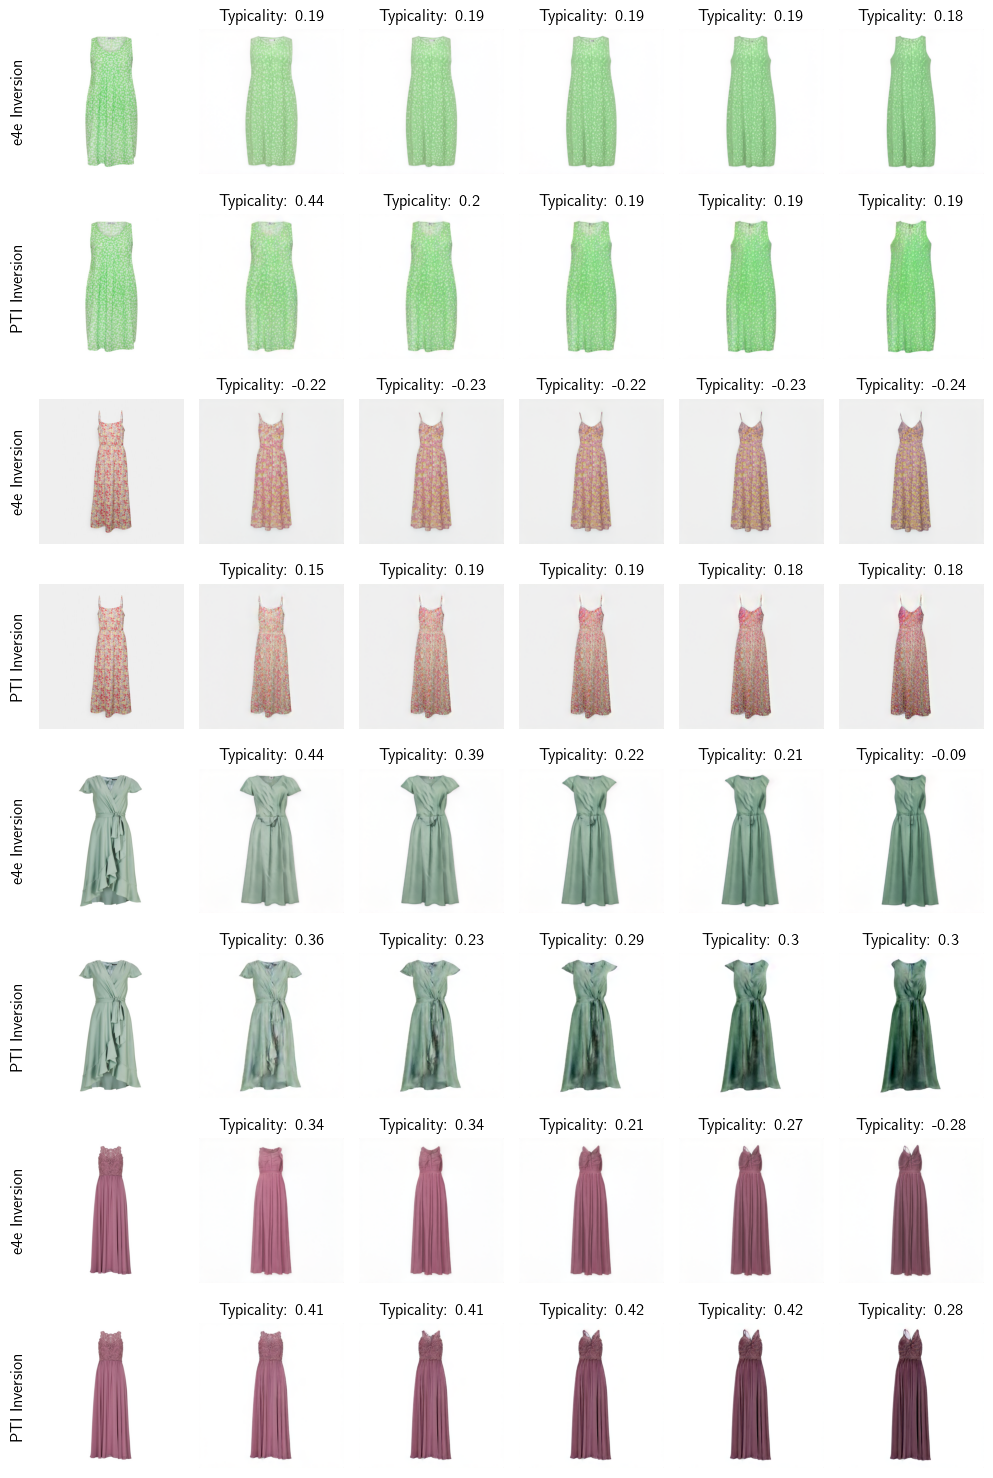
\includegraphics[width=0.9\linewidth]{Thesis/Results/assets/disentangled_less.png}
    \caption[Decreasing Typicality for Disentangled Embeddings]{Decreasing Typicality for Disentangled Embeddings: \textit{First row shows the original image, second row is the inversion. All following rows are each +5 InterFaceGAN steps towards less typicality}}
    \label{fig:disentangled_less}
\end{figure}

\clearpage
\begin{figure}[!ht]
    \centering
    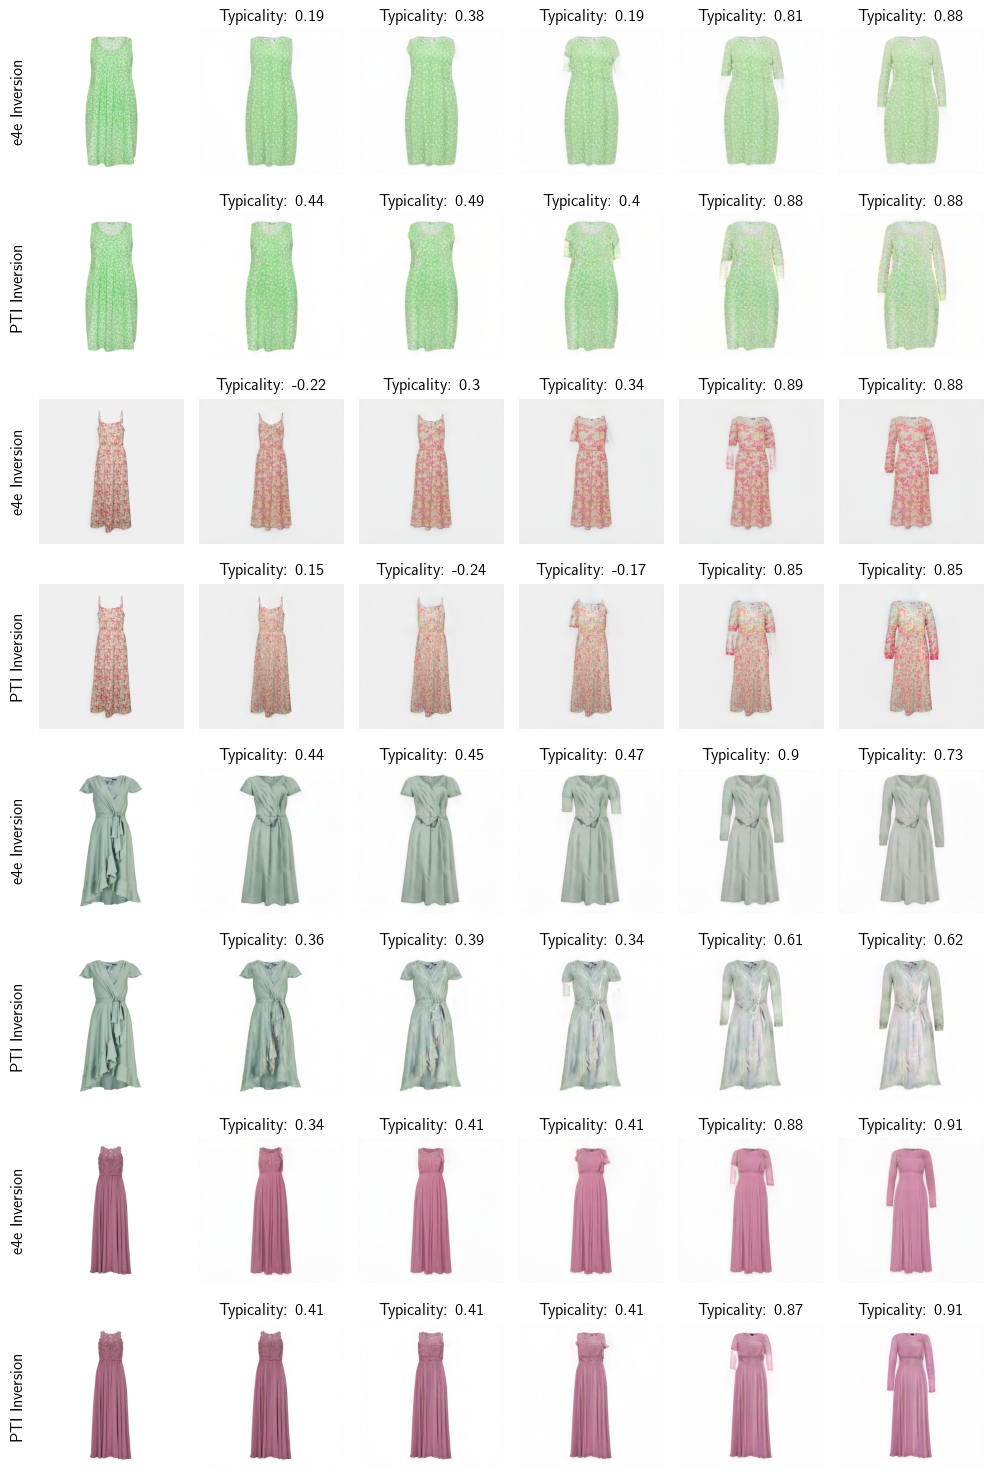
\includegraphics[width=0.9\linewidth]{Thesis/Results/assets/disentangled_more.png}
    \caption[Increasing Typicality for Disentangled Embeddings]{Increasing Typicality for Disentangled Embeddings: \textit{First row shows the original image, second row is the inversion. All following rows are each +5 InterFaceGAN steps towards more typicality}}
    \label{fig:disentangled_more}
\end{figure}

\clearpage
\begin{figure}[!ht]
    \centering
    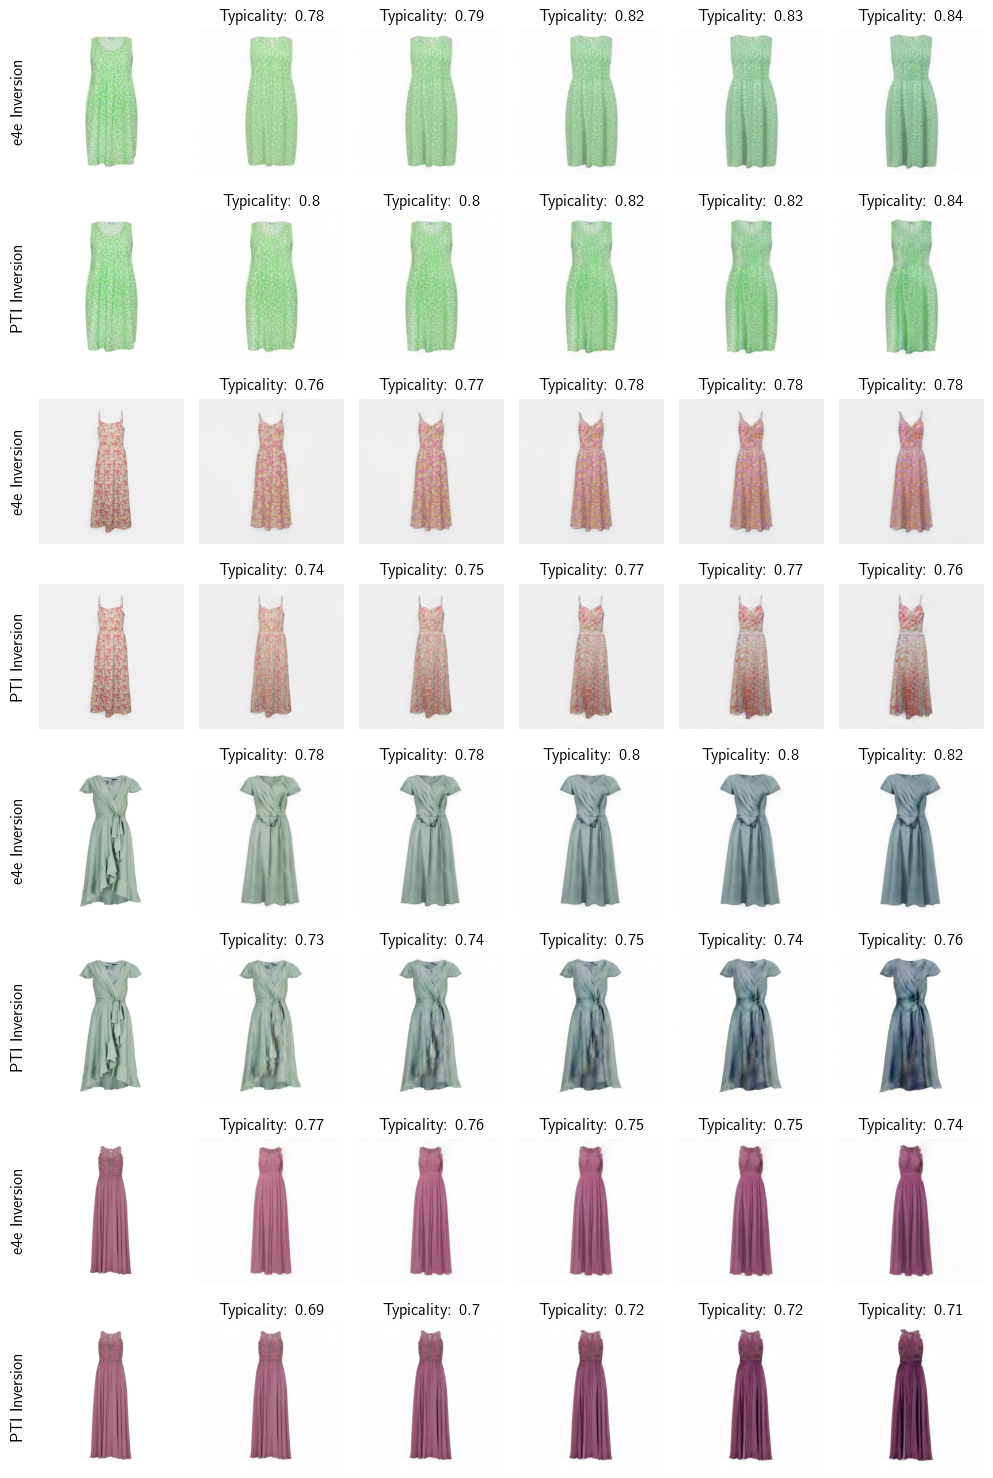
\includegraphics[width=0.9\linewidth]{Thesis/Results/assets/dino_cond_color_more.png}
    \caption[Increasing Typicality for DINOv2 Embeddings conditioned on Color]{Increasing Typicality for DINOv2 Embeddings conditioned on Color: \textit{First row shows the original image, second row is the inversion. All following rows are each +5 InterFaceGAN steps towards more typicality}}
    \label{fig:dino_cond_color_more}
\end{figure}

\clearpage
\begin{figure}[!ht]
    \centering
    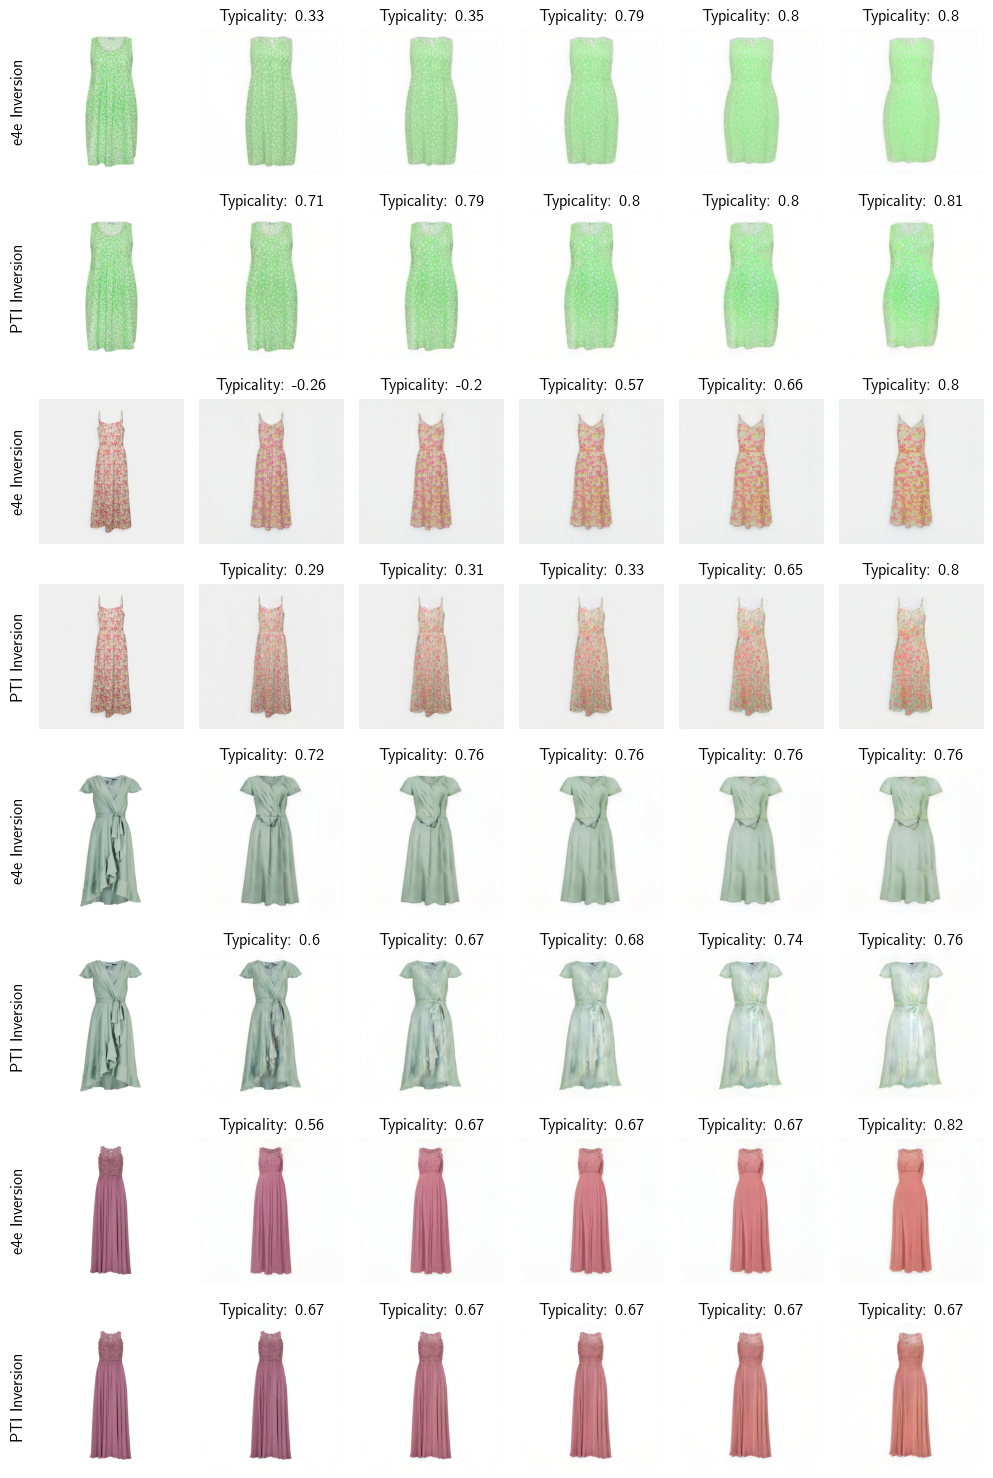
\includegraphics[width=0.9\linewidth]{Thesis/Results/assets/disentangled_ex_sleeve_more.png}
    \caption[Increasing Typicality for Disentangled Embeddings excl. Sleeve Length]{Increasing Typicality for Disentangled Embeddings excl. Sleeve Length: \textit{First row shows the original image, second row is the inversion. All following rows are each +5 InterFaceGAN steps towards more typicality}}
    \label{fig:disentangled_ex_sleeve_more}
\end{figure}

\clearpage
\begin{figure}[!ht]
    \centering
    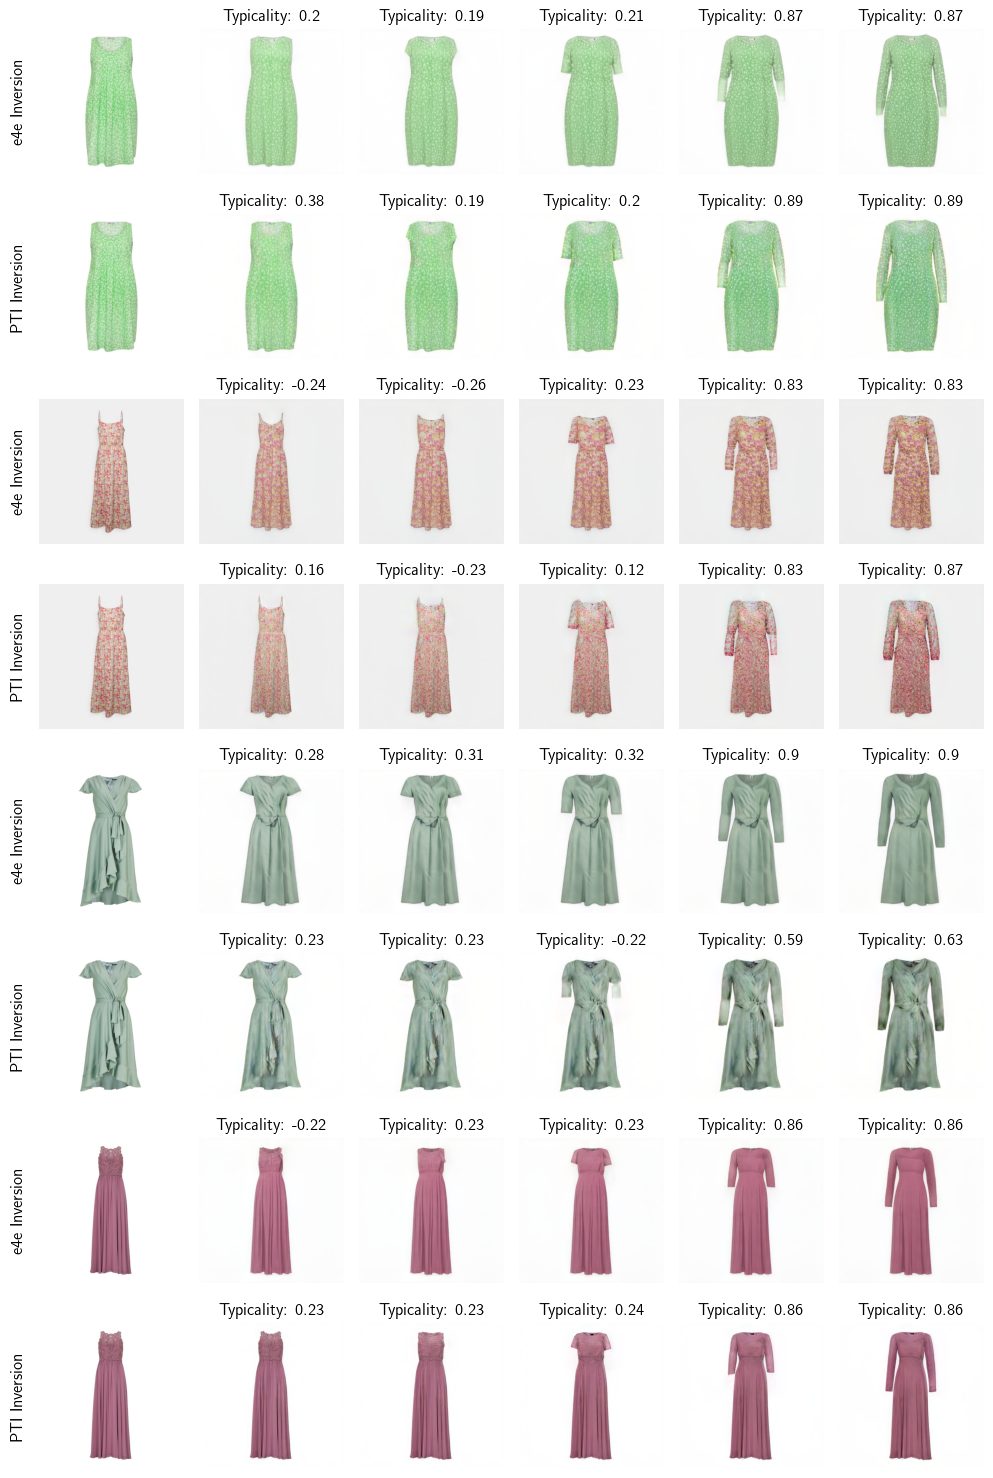
\includegraphics[width=0.9\linewidth]{Thesis/Results/assets/disentangled_ex_color_more.png}
    \caption[Increasing Typicality for Disentangled Embeddings excl. Color]{Increasing Typicality for Disentangled Embeddings excl. Color: \textit{First row shows the original image, second row is the inversion. All following rows are each +5 InterFaceGAN steps towards more typicality}}
    \label{fig:disentangled_ex_color_more}
\end{figure}






\clearpage

\vspace*{3cm}

\begin{center}
    \begin{minipage}{0.8\textwidth}
        \textbf{\large{Eidesstattliche Erklärung}}\\[1cm]
    
        Ich versichere an Eides Statt, dass ich die Arbeit selbständig verfasst, keine anderen als die angegebenen Hilfsmittel und Quellen benutzt habe, alle wörtlich oder sinngemäß aus anderen Werken übernommenen Aussagen als solche gekennzeichnet habe und dass die Arbeit weder vollständig noch in wesentlichen Teilen Gegenstand eines anderen Prüfungsverfahrens gewesen ist und dass ich die Arbeit weder vollständig noch in wesentlichen Teilen bereits veröffentlicht habe, sowie dass das in Dateiform eingereichte Exemplar mit den eingereichten gebundenen Exemplaren übereinstimmt.\\[1,5cm]

        Datum \hfill Unterschrift
    \end{minipage}
\end{center}


\thispagestyle{empty}

\newpage

\end{document}
